\chapter{Experiment}
\label{chap:experiment}
In this chapter we discuss the application of our approach from Chapter~\ref{chap:approach} using an experiment. We describe how we setup and conduct our experiment in Section~\ref{sec:experiment_setup}. We describe the selected test subjects using general metrics in Section~\ref{sec:experiment_subjects}. Finally we display our experimental results in Section~\ref{sec:experiment_results}.


\section{Experimental Setup}
\label{sec:experiment_setup}
We run our approach on a machine that has 6 GB of \gls{ram} and an Intel Core i7-870 processor running at 2.93 GHz. We have configured Javalanche to run with no parallel task execution along with its coverage impact analysis. We avoid task parallelization as it avoids any unnecessary issues that can occur due to concurrent access to file resources that a test suite may use. The coverage impact analysis slows down Javalanche though it provides comprehensive data regarding the mutants.

For each test subject we import the project into Eclipse and run the project through a \emph{test} that Javalanche provides. This test indicates any unit test cases that cannot execute properly or fail within Javalanche. We have to remove these test cases as the mutation testing process requires a test suite with no errors. We collect all the results in a database so we can conduct several forms of evaluation.

Using the common classifier performance measures as described in Section~\ref{subsec:background_performance_measures} we can quantifier how well the classifier does at prediction. We perform 10-fold cross-validation as described in Section~\ref{sec:background_machine_learning}. We also observe the performance of the classifier on real predictions by training on a subset of the available data then predicting on the remaining subset. LIBSVM provides an \emph{easy script} that automatically scale the data and make parameter selection using a grid search~\cite{HCL03}. Parameter selection is critical aspect of machine learning algorithms, it can influence the classification accuracy greatly. We allow LIBSVM to automatically take care of this to best select the parameters based on the provided data. We allow LIBSVM to use 8 threads for computation tasks. We also utilize the \gls{rbf} kernel as it is the default and comes recommended by the authors~\cite{HCL03}.


\section{Experimental Subjects}
\label{sec:experiment_subjects}
Our selection criteria for the experimental subjects were the following:

\begin{itemize}
  \item An open source Java software system.
  \item Contains a test suite or set of test cases.
  \item Is over 5K total \gls{sloc}.
\end{itemize}

We only wanted software system that have a minimum of 5K total \gls{sloc} to ensure that the our approach would gather a decent amount of data. Open source projects are relatively easy to find and are freely available to analyze. The only firm requirement we desired was the need for a test suite or set of test cases, due to fundamental needs of mutation testing.

\begin{landscape}
  \begin{table}[t]
    \centering
    \rowcolors{2}{gray!30}{gray!20}
    \begin{tabular}{|l|>{\raggedleft\arraybackslash}p{1.9cm}|>{\raggedleft\arraybackslash}p{1.9cm}|>{\raggedleft\arraybackslash}p{1.9cm}|>{\raggedleft\arraybackslash}p{1.9cm}|>{\raggedleft\arraybackslash}p{1.9cm}|>{\raggedleft\arraybackslash}p{1.9cm}|>{\raggedleft\arraybackslash}p{1.9cm}|}
      \hline
      \rowcolor[RGB]{169,196,223}
      \textbf{Program} & \textbf{Source SLOC} & \textbf{Source Classes} & \textbf{Source Methods} & \textbf{Test SLOC} & \textbf{Test Classes} & \textbf{Test Methods} & \textbf{Test Cases} \\
      \hline logback-core (1.0.3)~\cite{logback} & 12118 & 249 & 1270 & 8377 & 174 & 688 & 286 \\
      \hline barbecue (1.5-beta1)~\cite{barbecue} & 4790 & 58 & 299 & 2910 & 38 & 416 & 225 \\
      \hline jgap (3.6.1)~\cite{jgap} & 28975 & 415 & 3017 & 19694 & 180 & 1633 & 1355 \\
      \hline commons-lang (3.1)~\cite{commons-lang} & 19499 & 149 & 1196 & 33332 & 242 & 2408 & 2050 \\
      \hline joda-time (2.0)~\cite{joda-time} & 27139 & 227 & 3635 & 51388 & 221 & 4755 & 3866 \\
      \hline openfast (1.1.0)~\cite{openfast} & 11646 & 265 & 1447 & 5587 & 115 & 421 & 322 \\
      \hline jsoup (1.6.2)~\cite{jsoup} & 10949 & 198 & 954 & 2883 & 25 & 335 & 319 \\
      \hline joda-primitives (1.0)~\cite{joda-primitives} & 11157 & 128 & 1868 & 6989 & 49 & 746 & 1810 \\
      \hline \textbf{ALL} & \textbf{126273} & \textbf{1689} & \textbf{13686} & \textbf{131160} & \textbf{1044} & \textbf{11402} & \textbf{10233} \\
      \hline
    \end{tabular}
    \caption{The set of experimental subjects along with source and test metrics.}
    \vspace{2mm}
    \hrule
    \label{tab:experimental_subjects}
  \end{table}
\end{landscape}

Following the criteria outlined we selected the following 8 open source Java projects shown in Table~\ref{tab:experimental_subjects}. We provide a brief description of each project:

\begin{itemize}
  \item \textbf{logback-core}: \emph{``Logback is intended as a successor to the popular log4j project, picking up where log4j leaves off. The logback-core module lays the groundwork for the other two modules.''}~\cite{logback}
  \item \textbf{barbecue}: \emph{``Barbecue is an open-source, Java library that provides the means to create barcodes for printing and display in Java applications.''}~\cite{barbecue}
  \item \textbf{jgap}: \emph{``JGAP is a Genetic Algorithms and Genetic Programming component provided as a Java framework.''}~\cite{jgap}
  \item \textbf{commons-lang}: \emph{``The standard Java libraries fail to provide enough methods for manipulation of its core classes. Apache Commons Lang provides these extra methods.''}\cite{commons-lang}
  \item \textbf{joda-time}: \emph{``Joda-Time provides a quality replacement for the Java date and time classes. The design allows for multiple calendar systems, while still providing a simple API.''}~\cite{joda-time}
  \item \textbf{openfast}: \emph{``OpenFAST is a 100\% Java implementation of the FAST Protocol (FIX Adapted for STreaming). The FAST protocol is used to optimize communications in the electronic exchange of financial data.''}~\cite{openfast}
  \item \textbf{jsoup}: \emph{``jsoup is a Java library for working with real-world HTML. It provides a very convenient API for extracting and manipulating data, using the best of DOM, CSS, and jquery-like methods.''}~\cite{jsoup}
  \item \textbf{joda-primitives}: \emph{``Joda Primitives provides collections and utilities to bridge the gap between objects and primitive types in Java.''}~\cite{joda-primitives}
\end{itemize}

We use these experimental subjects in combination while collecting results. We consider an \emph{all} set which contains the data from all individual subjects, this allows us to observe the results using an amalgamation of subjects. We also consider subsets of the \emph{all} set by omitting a different subject for each subset (i.e., \emph{all\_but\_<subject>}), this allows us to perform predictions on a completely unknown subject using that data of the 7 other subjects.


\section{Experimental Results}
\label{sec:experiment_results}
Our results are broken up into separate sections:

\begin{itemize}
  \item \textbf{Mutation Score Distribution (Section~\ref{subsec:experiment_mutation_score_distribution})}: We discuss the results of the mutation score collection of the source code units. This section outlines the raw data and observations regarding the distribution of mutation scores. In particular we identify a suitable category abstraction for the mutation scores before moving forward to training and prediction using a \gls{svm}.
  \item \textbf{Cross Validation (Section~\ref{subsec:experiment_cross_validation})}: We discuss the cross-validation accuracy of our data sets. We present the cross-validation accuracy results with respect to the feature sets outlined in Table~\ref{tab:metrics}.
  \item \textbf{Prediction (Section~\ref{subsec:experiment_prediction})}: We discuss our approach and results on predicting unknown subjects using the collected data from our subjects.
  \item \textbf{Optimization \& Generalization (Section~\ref{subsec:experiment_optimization_generalization})}: We discuss the benefits of finding a generalizable set of parameters that fit our prediction purposes as well as optimizations to our feature set. We then re-evaluate the prediction accuracy using generalized parameters.
\end{itemize}


\subsection{Mutation Score Distribution}
\label{subsec:experiment_mutation_score_distribution}
\begin{landscape}
  \begin{table}[]
    \centering
    \rowcolors{1}{gray!30}{gray!20}
    \begin{threeparttable}
      \begin{tabular}{|l|>{\raggedleft}p{2.5cm}|>{\raggedleft}p{2.5cm}|>{\raggedleft}p{2.5cm}|>{\raggedleft}p{2.5cm}|>{\raggedleft}p{2.5cm}|>{\raggedleft\arraybackslash}p{2.5cm}|}
        \rowcolor[RGB]{169,196,223}
        \hline & \textbf{Mutants Generated} & \textbf{Mutants Covered} & \textbf{Coverage Percent} & \textbf{Mutants Killed} & \textbf{Mutation Score\tnote{a}} & \textbf{Time Taken (\emph{hh:mm:ss})} \\
        \hline \cellcolor[RGB]{169,196,223} \textbf{logback-core} & 10682 & 7350 & 0.6881 & 5400 & 0.7347 & 01:49:10 \\
        \hline \cellcolor[RGB]{169,196,223} \textbf{barbecue} & 27324 & 4339 & 0.1588 & 2727 & 0.6285 & 00:49:51 \\
        \hline \cellcolor[RGB]{169,196,223} \textbf{jgap} & 31929 & 17903 & 0.5607 & 13328 & 0.7445 & 07:04:44 \\
        \hline \cellcolor[RGB]{169,196,223} \textbf{commons-lang} & 45141 & 41761 & 0.9251 & 33772 & 0.8087 & 15:51:59 \\
        \hline \cellcolor[RGB]{169,196,223} \textbf{joda-time} & 70594 & 58595 & 0.8300 & 48545 & 0.8285 & 31:55:50 \\
        \hline \cellcolor[RGB]{169,196,223} \textbf{openfast} & 14910 & 8371 & 0.5614 & 6869 & 0.8206 & 01:34:38 \\
        \hline \cellcolor[RGB]{169,196,223} \textbf{jsoup} & 14165 & 10540 & 0.7441 & 8430 & 0.7998 & 03:55:56 \\
        \hline \cellcolor[RGB]{169,196,223} \textbf{joda-primitives} & 22269 & 17334 & 0.7784 & 13499 & 0.7788 & 01:24:33 \\
        \hline \cellcolor[RGB]{169,196,223} \textbf{ALL} & \textbf{237014} & \textbf{166193} & \textbf{0.7012} & \textbf{132570} & \textbf{0.7786} & \textbf{64:26:41} \\
        \hline
      \end{tabular}
      \begin{tablenotes}
        \item[a] Mutation score is calculated using the covered and killed mutants.
      \end{tablenotes}
    \end{threeparttable}
    \caption{Mutation testing results of the experimental subjects from table~\ref{tab:experimental_subjects}.}
    \vspace{2mm}
    \hrule
    \label{tab:experiments_mutation_results}
  \end{table}

  \begin{table}[ht!]
    \centering
    \rowcolors{1}{gray!30}{gray!20}
    \begin{threeparttable}
      \begin{tabular}{|l|r|r|}
        \rowcolor[RGB]{169,196,223}
        \hline & \textbf{Class-Level} & \textbf{Method-Level} \\
        \hline \cellcolor[RGB]{169,196,223} \textbf{logback-core} & 115 & 447 \\
        \hline \cellcolor[RGB]{169,196,223} \textbf{barbecue} & 31 & 143 \\
        \hline \cellcolor[RGB]{169,196,223} \textbf{jgap} & 124 & 655 \\
        \hline \cellcolor[RGB]{169,196,223} \textbf{commons-lang} & 124 & 789 \\
        \hline \cellcolor[RGB]{169,196,223} \textbf{joda-time} & 194 & 2019 \\
        \hline \cellcolor[RGB]{169,196,223} \textbf{openfast} & 120 & 401 \\
        \hline \cellcolor[RGB]{169,196,223} \textbf{jsoup} & 83 & 381 \\
        \hline \cellcolor[RGB]{169,196,223} \textbf{joda-primitives} & 73 & 675 \\
        \hline \cellcolor[RGB]{169,196,223} \textbf{ALL} & \textbf{864} & \textbf{5510} \\
        \hline
      \end{tabular}
    \end{threeparttable}
    \caption{The usable number of source code unit data points gathered from the experimental subjects in table~\ref{tab:experimental_subjects}.}
    \vspace{2mm}
    \hrule
    \label{tab:experiments_collected_data}
  \end{table}
\end{landscape}

As described in Chapter~\ref{chap:approach} our approach uses mutation testing to acquire the necessary mutation score data used for the category of the source code units. Table~\ref{tab:experiments_mutation_results} shows the results of running Javalanche on our experimental subjects. In all of our subjects mutation testing produced a large number of mutants that were evaluated, taking just over 64 hours for the entire mutation testing process. As described in Section~\ref{subsec:background_mutation_tools} Javalanche utilizes \emph{coverage} (i.e., basic block coverage) for test selection, which limits the number of mutants to evaluate to a subset of covered mutants. In most cases Javalanche was able to kill a reasonable percentage of the covered mutants with a mutation score of 0.7786 using all projects cumulatively. From the table we can see that the mutation scores of the individual projects are mostly above 0.7 which is a good indication that the test suites for covered source code units are reasonably effective. The coverage percent overall is 0.7012 which indicates that the test suites of the projects did not cover about 30\% of the generated mutants. Realistically mutation test works off of the entire project's source code, for our purpose only covered mutants were used to calculate the mutation score. The corrective action for non-covered mutants (i.e., mutants not covered by test suite using basic block coverage) is to add new test cases that provide coverage over the mutant's location.

\begin{figure}[ht!]
  \centering
  \begin{tikzpicture}
  \begin{axis}[
      bar width=1,
      ymajorgrids=true,
      xlabel=Mutation Score (\%),
      ylabel=\# of Classes,
      width=\linewidth,
      height=9.0cm]
      \addplot[ybar,fill=black] file {plots/all/evaluation_projects_class_distribution.txt};
  \end{axis}
  \end{tikzpicture}
  \caption{Mutation score distribution of classes from all 8 subjects from Table~\ref{tab:experimental_subjects} that can be used for training.}
  \vspace{2mm}
  \hrule
  \label{fig:mutation_distributions_class_all}
\end{figure}

\begin{figure}[ht!]
  \centering
  \begin{tikzpicture}
  \begin{axis}[
      bar width=1,
      ymajorgrids=true,
      xlabel=Mutation Score (\%),
      ylabel=\# of Methods,
      width=\linewidth,
      height=9.0cm]
      \addplot[ybar,fill=black] file {plots/all/evaluation_projects_method_distribution.txt};
  \end{axis}
  \end{tikzpicture}
  \caption{Mutation score distribution of methods from all 8 subjects from Table~\ref{tab:experimental_subjects} that can be used for training.}
  \vspace{2mm}
  \hrule
  \label{fig:mutation_distributions_method_all}
\end{figure}

\begin{figure}[ht!]
  \centering
  \begin{tikzpicture}
  \begin{axis}[
      xtick={0, 25, 50, 75, 100, 125, 150, 175, 200},
      xticklabels={0, 25, 50, 75, 100, 125, 150, 175, 200>=},
      bar width=1,
      ymajorgrids=true,
      xlabel=\# of Covered Mutants,
      ylabel=\# of Classes,
      width=\linewidth,
      height=9.0cm]
      \addplot[ybar,fill=black] file {plots/all/covered_mutants_class_distribution.txt};
  \end{axis}
  \end{tikzpicture}
  \caption{Covered mutant distribution of classes from all 8 subjects from Table~\ref{tab:experimental_subjects} that can be used for training.}
  \vspace{1mm}
  \footnotesize{\emph{Figure~\ref{fig:covered_mutant_distributions_class_all} only presents a subset of the full distribution, with the excluded values added on the last visible value. The max number of covered mutants found was 6507, which corresponds to the following class \texttt{org.joda.time.format.ISODateTimeFormat} from the \texttt{joda-time} project.}}
  \vspace{2mm}
  \hrule
  \label{fig:covered_mutant_distributions_class_all}
\end{figure}

\begin{figure}[ht!]
  \centering
  \begin{tikzpicture}
  \begin{axis}[
      xtick={0, 25, 50, 75, 100, 125, 150, 175, 200},
      xticklabels={0, 25, 50, 75, 100, 125, 150, 175, 200>=},
      bar width=1,
      ymajorgrids=true,
      xlabel=\# of Covered Mutants,
      ylabel=\# of Methods,
      width=\linewidth,
      height=9.0cm]
      \addplot[ybar,fill=black] file {plots/all/covered_mutants_method_distribution.txt};
  \end{axis}
  \end{tikzpicture}
  \caption{Covered mutant distribution of methods from all 8 subjects from Table~\ref{tab:experimental_subjects} that can be used for training.}
  \vspace{1mm}
  \footnotesize{\emph{Figure~\ref{fig:covered_mutant_distributions_method_all} only presents a subset of the full distribution, with the excluded values added on the last visible value. The max number of covered mutants found was 587, which corresponds to the following method \texttt{org.joda.time.format.PeriodFormatterBuilder\$FieldFormatter.parseInto} from the \texttt{joda-time} project. There were also 51 methods that had 117 covered mutants, of these 48 all fall within the \texttt{ISODateTimeFormat} class within the \texttt{joda-time} project.}}
  \vspace{2mm}
  \hrule
  \label{fig:covered_mutant_distributions_method_all}
\end{figure}

Source code and test code metrics were collected as described in Chapter~\ref{chap:approach} which represents the set of feature data that make up the vectors of our \gls{svm}. Our approach can only make predictions using the synthesis of both mutation score data (i.e., category data) and source and test suite metrics (i.e., feature data) of source code units. If any piece of data is missing then we cannot use that source code unit for training and prediction purposes. Using our approach we collected data for 864 class-level and 5510 method-level source code units shown in Table~\ref{tab:experiments_collected_data}. The collected data items is lower then the total available methods and classes, this is because: we ignore abstract, anonymous and overloaded source code units, as well as any source units with missing data (i.e., no tests cases). We present the distribution of the all the collected data points for both class-level and method-level source code units with respect to mutation score in Figure~\ref{fig:mutation_distributions_class_all}~\&~\ref{fig:mutation_distributions_method_all}. The mutation score distributions for each individual project are found in Appendix~\ref{app:mutation_score_distributions}. The mutation distribution of the both class-level and method-level source code units are both negatively skewed which confirms our earlier observation that the test suite for the collected source code units are reasonably strong at detecting faults. The 0\%, 50\% and 100\% values for mutation score contain significantly more data points then their surroundings, in particular the 100\% is ranges 2--9 times more dense then other areas respectively. We speculate this occurs because a large number of source code units probably have small number of covered mutants (i.e., easier to kill all, evenly kill half, kill none). Analysis of the covered mutant distribution for class-level source code units (as seen in Figure~\ref{fig:covered_mutant_distributions_method_all}) shows a slightly denser grouping for low covered mutants. The covered mutant distribution for method-level source code units supports our speculation, the distribution is positively skewed. With respect to the percentile of the class-level distribution of covered mutants a \sfrac{1}{4} of the classes have less then 16 covered mutants. The method-level results show that \sfrac{1}{4} of the methods have less then 2 covered mutants, furthermore \sfrac{1}{2} of the method have less then 6 covered mutants. With distributions like this we can assure that our speculation of many low covered mutant that can contribute to the high 0\%, 50\% and 100\% values for mutation score.

Earlier in Section~\ref{subsec:approach_create_libsvm_file} we mentioned that our approached would create \emph{.libsvm} files using the acquire data. The category data required for the files that the \gls{svm} utilizes is based on the mutation score of source code units. To avoid predicting the exact mutation score which is a set of real numbers, we instead use an abstracted set of categories (i.e., ranges of mutation scores). We were unsure on how to properly select the ranges to use for our categories. We decided to base our categories on the distribution of mutation scores from Figure~\ref{fig:covered_mutant_distributions_class_all}~\&~\ref{fig:covered_mutant_distributions_method_all}. We found that the class-level distribution has a 25$^{th}$, 50$^{th}$ and 75$^{th}$ percentile of 0.72, 0.81, 0.89 respectively, and for same percentiles of the method-level distribution are 0.75, 0.87, 0.99. Using these values we decided to use the following as our general case for categories:

\begin{itemize}
  \item \textbf{LOW} = [0.00--0.70)
  \item \textbf{MEDIUM} = [0.70--0.90)
  \item \textbf{HIGH} = [0.90--1.00]
\end{itemize}

The rational behind the categories is separate the lower and upper percentiles in to the LOW and HIGH category, with the remaining into the MEDIUM category. We believe that these values will provide a sufficient level of information over the mutation testing coverage of the source code units.


\subsection{Cross Validation}
\label{subsec:experiment_cross_validation}
\begin{table}[ht!]
  \centering
  \rowcolors{2}{gray!30}{gray!20}
  \begin{tabular}{|l|>{\raggedleft\arraybackslash}p{3cm}|>{\raggedleft\arraybackslash}p{3cm}|>{\raggedleft\arraybackslash}p{3cm}|}
    \hline
    \rowcolor[RGB]{169,196,223}
    \textbf{Category} & \textbf{Mutation Score Range} & \textbf{Class-Level Units} & \textbf{Method-Level Units} \\
    \hline LOW & [0.00--0.70) & 191 & 1104 \\
    \hline MEDIUM & [0.70--0.90) & 459 & 1782 \\
    \hline HIGH & [0.90--1.00] & 214 & 2624 \\
    \hline
  \end{tabular}
  \caption{The available number of source code units that fall within the determined ranges of mutation scores.}
  \vspace{2mm}
  \label{tab:available_data}
\end{table}

Using the determined classification categories from the previous section we have imbalanced training data in each category for class- and method-level source code units as shown in Table~\ref{tab:available_data}. Imbalanced data can be problematic for training and predicting using machine learning techniques. With imbalanced data a classifier will heavily classify towards the majority category~\cite{BOSB10}. Barandela et al. indicate that there are three strategies to reduce the problem of imbalanced training data: Over-sample, under-sample, or internally bias the classification process~\cite{BVSF04}. It was shown that simple random under-sampling can be an effective solution (though not always the best) to this problem~\cite{Jap00,AKJ04}. As Akbani et al. mentioned \emph{``\ldots we are throwing away valid instances, which contain valuable information''}, therefore we might be limiting the ability to generalize to new unknown data~\cite{AKJ04}. The alternative is to perform over-sampling, as Batista et al. mention \emph{``\ldots random over-sampling can increase the likelihood of occurring overfitting, since it makes exact copies of the minority class examples''}~\cite{BPM04}. We decided to utilize random under-sampling as it provides a simple approach to dealing with imbalanced data. Furthermore the imbalanced data we have is not extremely severe with a ratio around 2:5, thus we believe we are not losing that much information by under-sampling our training data.

\begin{figure}[ht!]
  \centering
  \begin{adjustbox}{max size={.95\textwidth}{.95\textheight}}
    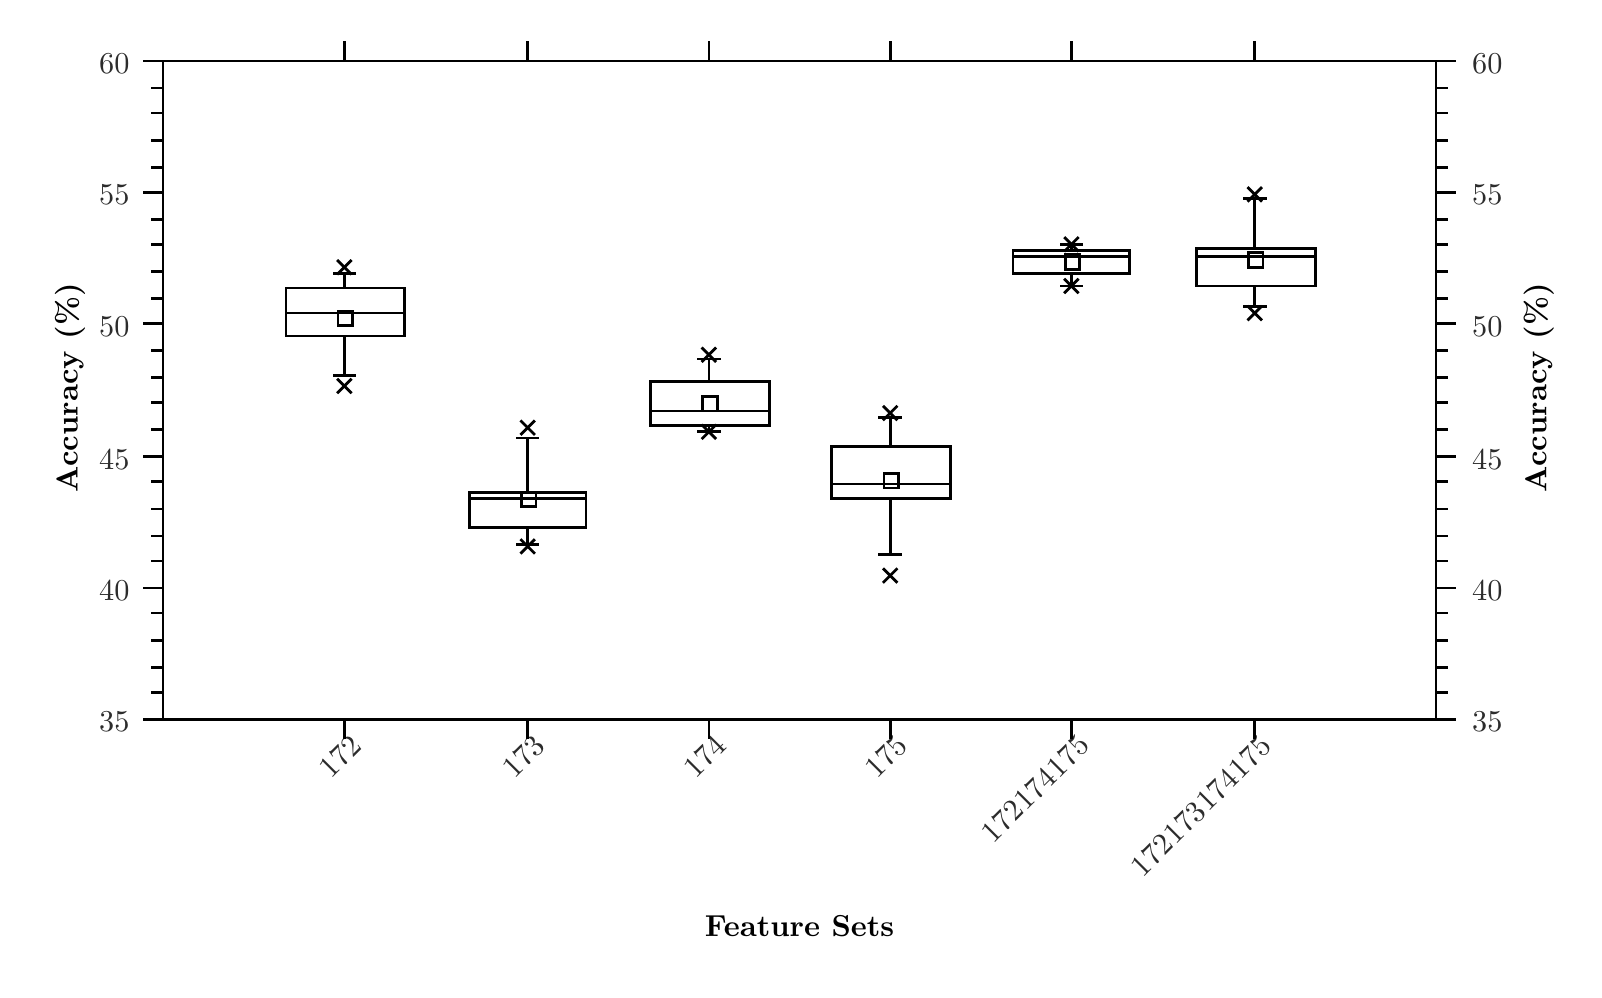
\begin{tikzpicture}{0pt}{0pt}{742pt}{452pt}
	\clip(0pt,452pt) -- (558.587pt,452pt) -- (558.587pt,111.729pt) -- (0pt,111.729pt) -- (0pt,452pt);
\begin{scope}
	\clip(48.9328pt,439.955pt) -- (508.901pt,439.955pt) -- (508.901pt,202.066pt) -- (48.9328pt,202.066pt) -- (48.9328pt,439.955pt);
	\color[rgb]{0,0,0}
	\draw[line width=1pt, line join=miter, line cap=rect](93.3487pt,357.898pt) -- (136.259pt,357.898pt) -- (136.259pt,340.584pt) -- (93.3487pt,340.584pt) -- (93.3487pt,357.898pt);
	\color[rgb]{0,0,0}
	\draw[line width=1pt, line join=miter, line cap=rect](110.663pt,326.28pt) -- (118.192pt,326.28pt);
	\draw[line width=1pt, line join=miter, line cap=rect](110.663pt,363.168pt) -- (118.192pt,363.168pt);
	\draw[line width=1pt, line join=miter, line cap=rect](114.427pt,363.168pt) -- (114.427pt,357.898pt);
	\draw[line width=1pt, line join=miter, line cap=rect](114.427pt,326.28pt) -- (114.427pt,340.584pt);
	\draw[line width=1pt, line join=miter, line cap=rect](93.3487pt,348.865pt) -- (135.506pt,348.865pt);
	\draw[line width=1pt, line join=miter, line cap=rect](112.169pt,324.775pt) -- (116.686pt,320.258pt);
	\draw[line width=1pt, line join=miter, line cap=rect](112.169pt,320.258pt) -- (116.686pt,324.775pt);
	\draw[line width=1pt, line join=miter, line cap=rect](112.169pt,367.685pt) -- (116.686pt,363.168pt);
	\draw[line width=1pt, line join=miter, line cap=rect](112.169pt,363.168pt) -- (116.686pt,367.685pt);
	\draw[line width=1pt, line join=miter, line cap=rect](112.169pt,349.618pt) -- (117.439pt,349.618pt) -- (117.439pt,344.348pt) -- (112.169pt,344.348pt) -- (112.169pt,349.618pt);
	\draw[line width=1pt, line join=miter, line cap=rect](159.596pt,284.123pt) -- (201.754pt,284.123pt) -- (201.754pt,271.325pt) -- (159.596pt,271.325pt) -- (159.596pt,284.123pt);
	\draw[line width=1pt, line join=miter, line cap=rect](176.911pt,265.303pt) -- (184.439pt,265.303pt);
	\draw[line width=1pt, line join=miter, line cap=rect](176.911pt,303.696pt) -- (184.439pt,303.696pt);
	\draw[line width=1pt, line join=miter, line cap=rect](180.675pt,303.696pt) -- (180.675pt,284.123pt);
	\draw[line width=1pt, line join=miter, line cap=rect](180.675pt,265.303pt) -- (180.675pt,271.325pt);
	\draw[line width=1pt, line join=miter, line cap=rect](159.596pt,281.864pt) -- (201.754pt,281.864pt);
	\draw[line width=1pt, line join=miter, line cap=rect](178.417pt,266.808pt) -- (182.933pt,262.291pt);
	\draw[line width=1pt, line join=miter, line cap=rect](178.417pt,262.291pt) -- (182.933pt,266.808pt);
	\draw[line width=1pt, line join=miter, line cap=rect](178.417pt,309.718pt) -- (182.933pt,305.202pt);
	\draw[line width=1pt, line join=miter, line cap=rect](178.417pt,305.202pt) -- (182.933pt,309.718pt);
	\draw[line width=1pt, line join=miter, line cap=rect](178.417pt,284.123pt) -- (183.686pt,284.123pt) -- (183.686pt,278.853pt) -- (178.417pt,278.853pt) -- (178.417pt,284.123pt);
	\draw[line width=1pt, line join=miter, line cap=rect](225.091pt,324.022pt) -- (268.001pt,324.022pt) -- (268.001pt,308.213pt) -- (225.091pt,308.213pt) -- (225.091pt,324.022pt);
	\draw[line width=1pt, line join=miter, line cap=rect](242.406pt,305.954pt) -- (249.934pt,305.954pt);
	\draw[line width=1pt, line join=miter, line cap=rect](242.406pt,332.303pt) -- (249.934pt,332.303pt);
	\draw[line width=1pt, line join=miter, line cap=rect](246.17pt,332.303pt) -- (246.17pt,324.022pt);
	\draw[line width=1pt, line join=miter, line cap=rect](246.17pt,305.954pt) -- (246.17pt,308.213pt);
	\draw[line width=1pt, line join=miter, line cap=rect](225.091pt,313.482pt) -- (267.248pt,313.482pt);
	\draw[line width=1pt, line join=miter, line cap=rect](243.911pt,308.213pt) -- (248.428pt,303.696pt);
	\draw[line width=1pt, line join=miter, line cap=rect](243.911pt,303.696pt) -- (248.428pt,308.213pt);
	\draw[line width=1pt, line join=miter, line cap=rect](243.911pt,336.067pt) -- (248.428pt,331.55pt);
	\draw[line width=1pt, line join=miter, line cap=rect](243.911pt,331.55pt) -- (248.428pt,336.067pt);
	\draw[line width=1pt, line join=miter, line cap=rect](243.911pt,318.752pt) -- (249.181pt,318.752pt) -- (249.181pt,313.482pt) -- (243.911pt,313.482pt) -- (243.911pt,318.752pt);
	\draw[line width=1pt, line join=miter, line cap=rect](290.586pt,300.685pt) -- (333.496pt,300.685pt) -- (333.496pt,281.864pt) -- (290.586pt,281.864pt) -- (290.586pt,300.685pt);
	\draw[line width=1pt, line join=miter, line cap=rect](307.9pt,261.538pt) -- (315.428pt,261.538pt);
	\draw[line width=1pt, line join=miter, line cap=rect](307.9pt,311.224pt) -- (315.428pt,311.224pt);
	\draw[line width=1pt, line join=miter, line cap=rect](311.664pt,311.224pt) -- (311.664pt,300.685pt);
	\draw[line width=1pt, line join=miter, line cap=rect](311.664pt,261.538pt) -- (311.664pt,281.864pt);
	\draw[line width=1pt, line join=miter, line cap=rect](290.586pt,287.134pt) -- (332.743pt,287.134pt);
	\draw[line width=1pt, line join=miter, line cap=rect](309.406pt,256.269pt) -- (313.923pt,251.752pt);
	\draw[line width=1pt, line join=miter, line cap=rect](309.406pt,251.752pt) -- (313.923pt,256.269pt);
	\draw[line width=1pt, line join=miter, line cap=rect](309.406pt,314.988pt) -- (313.923pt,310.471pt);
	\draw[line width=1pt, line join=miter, line cap=rect](309.406pt,310.471pt) -- (313.923pt,314.988pt);
	\draw[line width=1pt, line join=miter, line cap=rect](309.406pt,290.898pt) -- (314.676pt,290.898pt) -- (314.676pt,285.628pt) -- (309.406pt,285.628pt) -- (309.406pt,290.898pt);
	\draw[line width=1pt, line join=miter, line cap=rect](356.08pt,371.449pt) -- (398.238pt,371.449pt) -- (398.238pt,363.168pt) -- (356.08pt,363.168pt) -- (356.08pt,371.449pt);
	\draw[line width=1pt, line join=miter, line cap=rect](373.395pt,358.651pt) -- (380.923pt,358.651pt);
	\draw[line width=1pt, line join=miter, line cap=rect](373.395pt,373.707pt) -- (380.923pt,373.707pt);
	\draw[line width=1pt, line join=miter, line cap=rect](377.159pt,373.707pt) -- (377.159pt,371.449pt);
	\draw[line width=1pt, line join=miter, line cap=rect](377.159pt,358.651pt) -- (377.159pt,363.168pt);
	\draw[line width=1pt, line join=miter, line cap=rect](356.08pt,369.191pt) -- (398.238pt,369.191pt);
	\draw[line width=1pt, line join=miter, line cap=rect](374.901pt,360.91pt) -- (379.418pt,356.393pt);
	\draw[line width=1pt, line join=miter, line cap=rect](374.901pt,356.393pt) -- (379.418pt,360.91pt);
	\draw[line width=1pt, line join=miter, line cap=rect](374.901pt,375.966pt) -- (379.418pt,371.449pt);
	\draw[line width=1pt, line join=miter, line cap=rect](374.901pt,371.449pt) -- (379.418pt,375.966pt);
	\draw[line width=1pt, line join=miter, line cap=rect](374.901pt,369.943pt) -- (380.17pt,369.943pt) -- (380.17pt,364.674pt) -- (374.901pt,364.674pt) -- (374.901pt,369.943pt);
	\draw[line width=1pt, line join=miter, line cap=rect](422.328pt,372.202pt) -- (465.238pt,372.202pt) -- (465.238pt,358.651pt) -- (422.328pt,358.651pt) -- (422.328pt,372.202pt);
	\draw[line width=1pt, line join=miter, line cap=rect](439.642pt,351.123pt) -- (447.171pt,351.123pt);
	\draw[line width=1pt, line join=miter, line cap=rect](439.642pt,390.269pt) -- (447.171pt,390.269pt);
	\draw[line width=1pt, line join=miter, line cap=rect](443.407pt,390.269pt) -- (443.407pt,372.202pt);
	\draw[line width=1pt, line join=miter, line cap=rect](443.407pt,351.123pt) -- (443.407pt,358.651pt);
	\draw[line width=1pt, line join=miter, line cap=rect](422.328pt,369.191pt) -- (464.485pt,369.191pt);
	\draw[line width=1pt, line join=miter, line cap=rect](441.148pt,351.123pt) -- (445.665pt,346.606pt);
	\draw[line width=1pt, line join=miter, line cap=rect](441.148pt,346.606pt) -- (445.665pt,351.123pt);
	\draw[line width=1pt, line join=miter, line cap=rect](441.148pt,394.033pt) -- (445.665pt,389.517pt);
	\draw[line width=1pt, line join=miter, line cap=rect](441.148pt,389.517pt) -- (445.665pt,394.033pt);
	\draw[line width=1pt, line join=miter, line cap=rect](441.148pt,370.696pt) -- (446.418pt,370.696pt) -- (446.418pt,365.427pt) -- (441.148pt,365.427pt) -- (441.148pt,370.696pt);
\end{scope}
\begin{scope}
	\color[rgb]{0,0,0}
	\pgftext[center, base, at={\pgfpoint{18.0675pt}{321.763pt}},rotate=90]{\fontsize{11}{0}\selectfont{\textbf{Accuracy (\%)}}}
	\color[rgb]{0.172549,0.172549,0.172549}
	\pgftext[center, base, at={\pgfpoint{31.3358pt}{197.549pt}}]{\fontsize{11}{0}\selectfont{35}}
	\pgftext[center, base, at={\pgfpoint{31.3358pt}{244.977pt}}]{\fontsize{11}{0}\selectfont{40}}
	\pgftext[center, base, at={\pgfpoint{31.3358pt}{292.404pt}}]{\fontsize{11}{0}\selectfont{45}}
	\pgftext[center, base, at={\pgfpoint{31.3358pt}{340.584pt}}]{\fontsize{11}{0}\selectfont{50}}
	\pgftext[center, base, at={\pgfpoint{31.3358pt}{388.011pt}}]{\fontsize{11}{0}\selectfont{55}}
	\pgftext[center, base, at={\pgfpoint{31.3358pt}{435.438pt}}]{\fontsize{11}{0}\selectfont{60}}
	\color[rgb]{0,0,0}
	\draw[line width=1pt, line join=bevel, line cap=rect](48.9328pt,211.853pt) -- (45.1688pt,211.853pt);
	\draw[line width=1pt, line join=bevel, line cap=rect](48.9328pt,220.887pt) -- (45.1688pt,220.887pt);
	\draw[line width=1pt, line join=bevel, line cap=rect](48.9328pt,230.673pt) -- (45.1688pt,230.673pt);
	\draw[line width=1pt, line join=bevel, line cap=rect](48.9328pt,240.46pt) -- (45.1688pt,240.46pt);
	\draw[line width=1pt, line join=bevel, line cap=rect](48.9328pt,259.28pt) -- (45.1688pt,259.28pt);
	\draw[line width=1pt, line join=bevel, line cap=rect](48.9328pt,268.314pt) -- (45.1688pt,268.314pt);
	\draw[line width=1pt, line join=bevel, line cap=rect](48.9328pt,278.1pt) -- (45.1688pt,278.1pt);
	\draw[line width=1pt, line join=bevel, line cap=rect](48.9328pt,287.887pt) -- (45.1688pt,287.887pt);
	\draw[line width=1pt, line join=bevel, line cap=rect](48.9328pt,306.707pt) -- (45.1688pt,306.707pt);
	\draw[line width=1pt, line join=bevel, line cap=rect](48.9328pt,316.494pt) -- (45.1688pt,316.494pt);
	\draw[line width=1pt, line join=bevel, line cap=rect](48.9328pt,325.528pt) -- (45.1688pt,325.528pt);
	\draw[line width=1pt, line join=bevel, line cap=rect](48.9328pt,335.314pt) -- (45.1688pt,335.314pt);
	\draw[line width=1pt, line join=bevel, line cap=rect](48.9328pt,354.134pt) -- (45.1688pt,354.134pt);
	\draw[line width=1pt, line join=bevel, line cap=rect](48.9328pt,363.921pt) -- (45.1688pt,363.921pt);
	\draw[line width=1pt, line join=bevel, line cap=rect](48.9328pt,373.707pt) -- (45.1688pt,373.707pt);
	\draw[line width=1pt, line join=bevel, line cap=rect](48.9328pt,382.741pt) -- (45.1688pt,382.741pt);
	\draw[line width=1pt, line join=bevel, line cap=rect](48.9328pt,401.562pt) -- (45.1688pt,401.562pt);
	\draw[line width=1pt, line join=bevel, line cap=rect](48.9328pt,411.348pt) -- (45.1688pt,411.348pt);
	\draw[line width=1pt, line join=bevel, line cap=rect](48.9328pt,421.135pt) -- (45.1688pt,421.135pt);
	\draw[line width=1pt, line join=bevel, line cap=rect](48.9328pt,430.168pt) -- (45.1688pt,430.168pt);
	\draw[line width=1pt, line join=bevel, line cap=rect](48.9328pt,202.066pt) -- (42.1575pt,202.066pt);
	\draw[line width=1pt, line join=bevel, line cap=rect](48.9328pt,249.493pt) -- (42.1575pt,249.493pt);
	\draw[line width=1pt, line join=bevel, line cap=rect](48.9328pt,296.921pt) -- (42.1575pt,296.921pt);
	\draw[line width=1pt, line join=bevel, line cap=rect](48.9328pt,345.101pt) -- (42.1575pt,345.101pt);
	\draw[line width=1pt, line join=bevel, line cap=rect](48.9328pt,392.528pt) -- (42.1575pt,392.528pt);
	\draw[line width=1pt, line join=bevel, line cap=rect](48.9328pt,439.955pt) -- (42.1575pt,439.955pt);
	\draw[line width=1pt, line join=bevel, line cap=rect](48.9328pt,439.955pt) -- (48.9328pt,202.066pt);
	\pgftext[center, base, at={\pgfpoint{548.8pt}{321.763pt}},rotate=90]{\fontsize{11}{0}\selectfont{\textbf{Accuracy (\%)}}}
	\color[rgb]{0.172549,0.172549,0.172549}
	\pgftext[center, base, at={\pgfpoint{527.439pt}{197.549pt}}]{\fontsize{11}{0}\selectfont{35}}
	\pgftext[center, base, at={\pgfpoint{527.439pt}{244.977pt}}]{\fontsize{11}{0}\selectfont{40}}
	\pgftext[center, base, at={\pgfpoint{527.439pt}{292.404pt}}]{\fontsize{11}{0}\selectfont{45}}
	\pgftext[center, base, at={\pgfpoint{527.439pt}{340.584pt}}]{\fontsize{11}{0}\selectfont{50}}
	\pgftext[center, base, at={\pgfpoint{527.439pt}{388.011pt}}]{\fontsize{11}{0}\selectfont{55}}
	\pgftext[center, base, at={\pgfpoint{527.439pt}{435.438pt}}]{\fontsize{11}{0}\selectfont{60}}
	\color[rgb]{0,0,0}
	\draw[line width=1pt, line join=bevel, line cap=rect](508.901pt,211.853pt) -- (512.665pt,211.853pt);
	\draw[line width=1pt, line join=bevel, line cap=rect](508.901pt,220.887pt) -- (512.665pt,220.887pt);
	\draw[line width=1pt, line join=bevel, line cap=rect](508.901pt,230.673pt) -- (512.665pt,230.673pt);
	\draw[line width=1pt, line join=bevel, line cap=rect](508.901pt,240.46pt) -- (512.665pt,240.46pt);
	\draw[line width=1pt, line join=bevel, line cap=rect](508.901pt,259.28pt) -- (512.665pt,259.28pt);
	\draw[line width=1pt, line join=bevel, line cap=rect](508.901pt,268.314pt) -- (512.665pt,268.314pt);
	\draw[line width=1pt, line join=bevel, line cap=rect](508.901pt,278.1pt) -- (512.665pt,278.1pt);
	\draw[line width=1pt, line join=bevel, line cap=rect](508.901pt,287.887pt) -- (512.665pt,287.887pt);
	\draw[line width=1pt, line join=bevel, line cap=rect](508.901pt,306.707pt) -- (512.665pt,306.707pt);
	\draw[line width=1pt, line join=bevel, line cap=rect](508.901pt,316.494pt) -- (512.665pt,316.494pt);
	\draw[line width=1pt, line join=bevel, line cap=rect](508.901pt,325.528pt) -- (512.665pt,325.528pt);
	\draw[line width=1pt, line join=bevel, line cap=rect](508.901pt,335.314pt) -- (512.665pt,335.314pt);
	\draw[line width=1pt, line join=bevel, line cap=rect](508.901pt,354.134pt) -- (512.665pt,354.134pt);
	\draw[line width=1pt, line join=bevel, line cap=rect](508.901pt,363.921pt) -- (512.665pt,363.921pt);
	\draw[line width=1pt, line join=bevel, line cap=rect](508.901pt,373.707pt) -- (512.665pt,373.707pt);
	\draw[line width=1pt, line join=bevel, line cap=rect](508.901pt,382.741pt) -- (512.665pt,382.741pt);
	\draw[line width=1pt, line join=bevel, line cap=rect](508.901pt,401.562pt) -- (512.665pt,401.562pt);
	\draw[line width=1pt, line join=bevel, line cap=rect](508.901pt,411.348pt) -- (512.665pt,411.348pt);
	\draw[line width=1pt, line join=bevel, line cap=rect](508.901pt,421.135pt) -- (512.665pt,421.135pt);
	\draw[line width=1pt, line join=bevel, line cap=rect](508.901pt,430.168pt) -- (512.665pt,430.168pt);
	\draw[line width=1pt, line join=bevel, line cap=rect](508.901pt,202.066pt) -- (515.677pt,202.066pt);
	\draw[line width=1pt, line join=bevel, line cap=rect](508.901pt,249.493pt) -- (515.677pt,249.493pt);
	\draw[line width=1pt, line join=bevel, line cap=rect](508.901pt,296.921pt) -- (515.677pt,296.921pt);
	\draw[line width=1pt, line join=bevel, line cap=rect](508.901pt,345.101pt) -- (515.677pt,345.101pt);
	\draw[line width=1pt, line join=bevel, line cap=rect](508.901pt,392.528pt) -- (515.677pt,392.528pt);
	\draw[line width=1pt, line join=bevel, line cap=rect](508.901pt,439.955pt) -- (515.677pt,439.955pt);
	\draw[line width=1pt, line join=bevel, line cap=rect](508.901pt,439.955pt) -- (508.901pt,202.066pt);
	\pgftext[center, base, at={\pgfpoint{278.911pt}{123.774pt}}]{\fontsize{11}{0}\selectfont{\textbf{Feature Sets}}}
	\color[rgb]{0.172549,0.172549,0.172549}
	\pgftext[center, base, at={\pgfpoint{115.392pt}{186.104pt}},rotate=45]{\fontsize{11}{0}\selectfont{\ding{172}}}
	\pgftext[center, base, at={\pgfpoint{181.64pt}{186.104pt}},rotate=45]{\fontsize{11}{0}\selectfont{\ding{173}}}
	\pgftext[center, base, at={\pgfpoint{247.135pt}{186.104pt}},rotate=45]{\fontsize{11}{0}\selectfont{\ding{174}}}
	\pgftext[center, base, at={\pgfpoint{312.629pt}{186.104pt}},rotate=45]{\fontsize{11}{0}\selectfont{\ding{175}}}
	\pgftext[center, base, at={\pgfpoint{354.702pt}{162.682pt}},rotate=45]{\fontsize{11}{0}\selectfont{\ding{172}}}
	\pgftext[center, base, at={\pgfpoint{366.513pt}{174.493pt}},rotate=45]{\fontsize{11}{0}\selectfont{\ding{174}}}
	\pgftext[center, base, at={\pgfpoint{378.324pt}{186.303pt}},rotate=45]{\fontsize{11}{0}\selectfont{\ding{175}}}
	\pgftext[center, base, at={\pgfpoint{408.706pt}{150.439pt}},rotate=45]{\fontsize{11}{0}\selectfont{\ding{172}}}
	\pgftext[center, base, at={\pgfpoint{420.517pt}{162.249pt}},rotate=45]{\fontsize{11}{0}\selectfont{\ding{173}}}
	\pgftext[center, base, at={\pgfpoint{432.328pt}{174.06pt}},rotate=45]{\fontsize{11}{0}\selectfont{\ding{174}}}
	\pgftext[center, base, at={\pgfpoint{444.139pt}{185.871pt}},rotate=45]{\fontsize{11}{0}\selectfont{\ding{175}}}
	\color[rgb]{0,0,0}
	\draw[line width=1pt, line join=bevel, line cap=rect](114.427pt,202.066pt) -- (114.427pt,195.291pt);
	\draw[line width=1pt, line join=bevel, line cap=rect](180.675pt,202.066pt) -- (180.675pt,195.291pt);
	\draw[line width=1pt, line join=bevel, line cap=rect](246.17pt,202.066pt) -- (246.17pt,195.291pt);
	\draw[line width=1pt, line join=bevel, line cap=rect](311.664pt,202.066pt) -- (311.664pt,195.291pt);
	\draw[line width=1pt, line join=bevel, line cap=rect](377.159pt,202.066pt) -- (377.159pt,195.291pt);
	\draw[line width=1pt, line join=bevel, line cap=rect](443.407pt,202.066pt) -- (443.407pt,195.291pt);
	\draw[line width=1pt, line join=bevel, line cap=rect](48.9328pt,202.066pt) -- (508.901pt,202.066pt);
	\draw[line width=1pt, line join=bevel, line cap=rect](114.427pt,439.955pt) -- (114.427pt,446.73pt);
	\draw[line width=1pt, line join=bevel, line cap=rect](180.675pt,439.955pt) -- (180.675pt,446.73pt);
	\draw[line width=1pt, line join=bevel, line cap=rect](246.17pt,439.955pt) -- (246.17pt,446.73pt);
	\draw[line width=1pt, line join=bevel, line cap=rect](311.664pt,439.955pt) -- (311.664pt,446.73pt);
	\draw[line width=1pt, line join=bevel, line cap=rect](377.159pt,439.955pt) -- (377.159pt,446.73pt);
	\draw[line width=1pt, line join=bevel, line cap=rect](443.407pt,439.955pt) -- (443.407pt,446.73pt);
	\draw[line width=1pt, line join=bevel, line cap=rect](48.9328pt,439.955pt) -- (508.901pt,439.955pt);
\end{scope}
\end{tikzpicture}

  \end{adjustbox}
  \caption{Class-level cross-validation accuracy of feature sets on the \emph{all} subject.}
  \vspace{2mm}
  \hrule
  \label{fig:all_cross_validation_features_class_graph}
\end{figure}

\begin{figure}[ht!]
  \centering
  \begin{adjustbox}{max size={.95\textwidth}{.95\textheight}}
    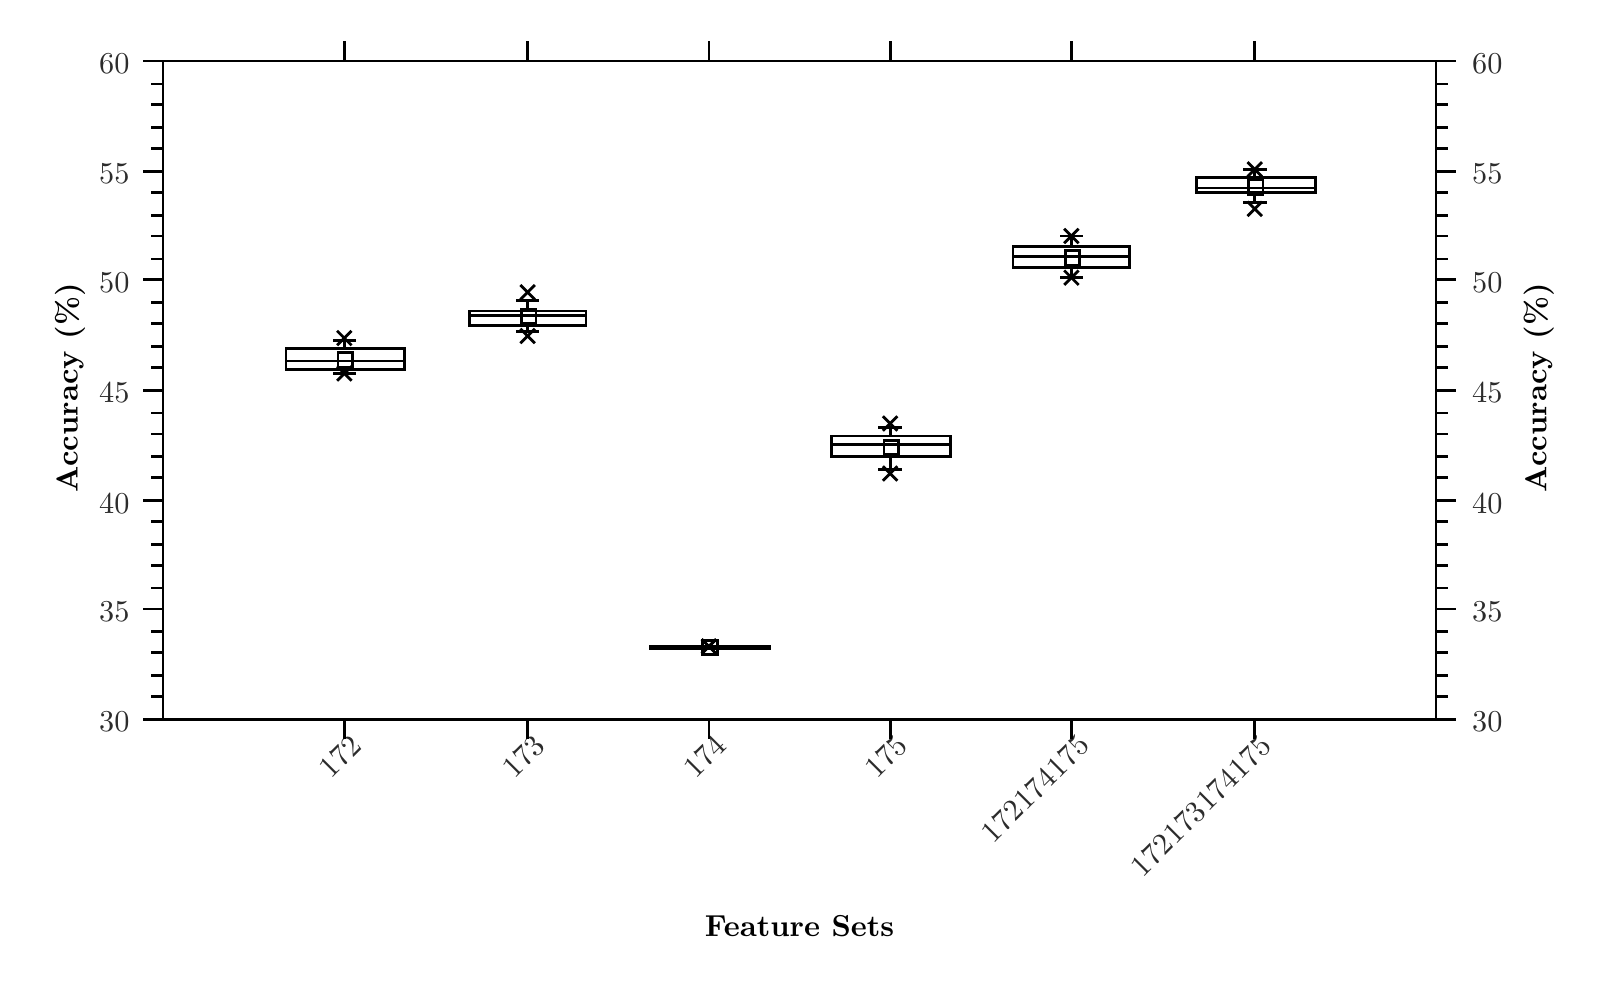
\begin{tikzpicture}{0pt}{0pt}{742pt}{452pt}
	\clip(0pt,452pt) -- (558.587pt,452pt) -- (558.587pt,111.729pt) -- (0pt,111.729pt) -- (0pt,452pt);
\begin{scope}
	\clip(48.9328pt,439.955pt) -- (508.901pt,439.955pt) -- (508.901pt,202.066pt) -- (48.9328pt,202.066pt) -- (48.9328pt,439.955pt);
	\color[rgb]{0,0,0}
	\draw[line width=1pt, line join=miter, line cap=rect](93.3487pt,336.067pt) -- (136.259pt,336.067pt) -- (136.259pt,328.539pt) -- (93.3487pt,328.539pt) -- (93.3487pt,336.067pt);
	\color[rgb]{0,0,0}
	\draw[line width=1pt, line join=miter, line cap=rect](110.663pt,327.033pt) -- (118.192pt,327.033pt);
	\draw[line width=1pt, line join=miter, line cap=rect](110.663pt,339.078pt) -- (118.192pt,339.078pt);
	\draw[line width=1pt, line join=miter, line cap=rect](114.427pt,339.078pt) -- (114.427pt,336.067pt);
	\draw[line width=1pt, line join=miter, line cap=rect](114.427pt,327.033pt) -- (114.427pt,328.539pt);
	\draw[line width=1pt, line join=miter, line cap=rect](93.3487pt,331.55pt) -- (135.506pt,331.55pt);
	\draw[line width=1pt, line join=miter, line cap=rect](112.169pt,329.292pt) -- (116.686pt,324.775pt);
	\draw[line width=1pt, line join=miter, line cap=rect](112.169pt,324.775pt) -- (116.686pt,329.292pt);
	\draw[line width=1pt, line join=miter, line cap=rect](112.169pt,342.089pt) -- (116.686pt,337.572pt);
	\draw[line width=1pt, line join=miter, line cap=rect](112.169pt,337.572pt) -- (116.686pt,342.089pt);
	\draw[line width=1pt, line join=miter, line cap=rect](112.169pt,334.561pt) -- (117.439pt,334.561pt) -- (117.439pt,329.292pt) -- (112.169pt,329.292pt) -- (112.169pt,334.561pt);
	\draw[line width=1pt, line join=miter, line cap=rect](159.596pt,349.618pt) -- (201.754pt,349.618pt) -- (201.754pt,344.348pt) -- (159.596pt,344.348pt) -- (159.596pt,349.618pt);
	\draw[line width=1pt, line join=miter, line cap=rect](176.911pt,342.089pt) -- (184.439pt,342.089pt);
	\draw[line width=1pt, line join=miter, line cap=rect](176.911pt,353.382pt) -- (184.439pt,353.382pt);
	\draw[line width=1pt, line join=miter, line cap=rect](180.675pt,353.382pt) -- (180.675pt,349.618pt);
	\draw[line width=1pt, line join=miter, line cap=rect](180.675pt,342.089pt) -- (180.675pt,344.348pt);
	\draw[line width=1pt, line join=miter, line cap=rect](159.596pt,348.112pt) -- (201.754pt,348.112pt);
	\draw[line width=1pt, line join=miter, line cap=rect](178.417pt,342.842pt) -- (182.933pt,338.325pt);
	\draw[line width=1pt, line join=miter, line cap=rect](178.417pt,338.325pt) -- (182.933pt,342.842pt);
	\draw[line width=1pt, line join=miter, line cap=rect](178.417pt,358.651pt) -- (182.933pt,354.134pt);
	\draw[line width=1pt, line join=miter, line cap=rect](178.417pt,354.134pt) -- (182.933pt,358.651pt);
	\draw[line width=1pt, line join=miter, line cap=rect](178.417pt,350.37pt) -- (183.686pt,350.37pt) -- (183.686pt,345.101pt) -- (178.417pt,345.101pt) -- (178.417pt,350.37pt);
	\draw[line width=1pt, line join=miter, line cap=rect](225.091pt,228.415pt) -- (268.001pt,228.415pt) -- (268.001pt,227.662pt) -- (225.091pt,227.662pt) -- (225.091pt,228.415pt);
	\draw[line width=1pt, line join=miter, line cap=rect](242.406pt,228.415pt) -- (249.934pt,228.415pt);
	\draw[line width=1pt, line join=miter, line cap=rect](242.406pt,228.415pt) -- (249.934pt,228.415pt);
	\draw[line width=1pt, line join=miter, line cap=rect](225.091pt,228.415pt) -- (267.248pt,228.415pt);
	\draw[line width=1pt, line join=miter, line cap=rect](243.911pt,230.673pt) -- (248.428pt,226.156pt);
	\draw[line width=1pt, line join=miter, line cap=rect](243.911pt,226.156pt) -- (248.428pt,230.673pt);
	\draw[line width=1pt, line join=miter, line cap=rect](243.911pt,230.673pt) -- (248.428pt,226.156pt);
	\draw[line width=1pt, line join=miter, line cap=rect](243.911pt,226.156pt) -- (248.428pt,230.673pt);
	\draw[line width=1pt, line join=miter, line cap=rect](243.911pt,230.673pt) -- (249.181pt,230.673pt) -- (249.181pt,225.403pt) -- (243.911pt,225.403pt) -- (243.911pt,230.673pt);
	\draw[line width=1pt, line join=miter, line cap=rect](290.586pt,304.449pt) -- (333.496pt,304.449pt) -- (333.496pt,296.921pt) -- (290.586pt,296.921pt) -- (290.586pt,304.449pt);
	\draw[line width=1pt, line join=miter, line cap=rect](307.9pt,292.404pt) -- (315.428pt,292.404pt);
	\draw[line width=1pt, line join=miter, line cap=rect](307.9pt,307.46pt) -- (315.428pt,307.46pt);
	\draw[line width=1pt, line join=miter, line cap=rect](311.664pt,307.46pt) -- (311.664pt,304.449pt);
	\draw[line width=1pt, line join=miter, line cap=rect](311.664pt,292.404pt) -- (311.664pt,296.921pt);
	\draw[line width=1pt, line join=miter, line cap=rect](290.586pt,301.438pt) -- (332.743pt,301.438pt);
	\draw[line width=1pt, line join=miter, line cap=rect](309.406pt,293.157pt) -- (313.923pt,288.64pt);
	\draw[line width=1pt, line join=miter, line cap=rect](309.406pt,288.64pt) -- (313.923pt,293.157pt);
	\draw[line width=1pt, line join=miter, line cap=rect](309.406pt,311.224pt) -- (313.923pt,306.707pt);
	\draw[line width=1pt, line join=miter, line cap=rect](309.406pt,306.707pt) -- (313.923pt,311.224pt);
	\draw[line width=1pt, line join=miter, line cap=rect](309.406pt,302.943pt) -- (314.676pt,302.943pt) -- (314.676pt,297.673pt) -- (309.406pt,297.673pt) -- (309.406pt,302.943pt);
	\draw[line width=1pt, line join=miter, line cap=rect](356.08pt,372.955pt) -- (398.238pt,372.955pt) -- (398.238pt,365.427pt) -- (356.08pt,365.427pt) -- (356.08pt,372.955pt);
	\draw[line width=1pt, line join=miter, line cap=rect](373.395pt,361.663pt) -- (380.923pt,361.663pt);
	\draw[line width=1pt, line join=miter, line cap=rect](373.395pt,376.719pt) -- (380.923pt,376.719pt);
	\draw[line width=1pt, line join=miter, line cap=rect](377.159pt,376.719pt) -- (377.159pt,372.955pt);
	\draw[line width=1pt, line join=miter, line cap=rect](377.159pt,361.663pt) -- (377.159pt,365.427pt);
	\draw[line width=1pt, line join=miter, line cap=rect](356.08pt,369.191pt) -- (398.238pt,369.191pt);
	\draw[line width=1pt, line join=miter, line cap=rect](374.901pt,363.921pt) -- (379.418pt,359.404pt);
	\draw[line width=1pt, line join=miter, line cap=rect](374.901pt,359.404pt) -- (379.418pt,363.921pt);
	\draw[line width=1pt, line join=miter, line cap=rect](374.901pt,378.977pt) -- (379.418pt,374.46pt);
	\draw[line width=1pt, line join=miter, line cap=rect](374.901pt,374.46pt) -- (379.418pt,378.977pt);
	\draw[line width=1pt, line join=miter, line cap=rect](374.901pt,371.449pt) -- (380.17pt,371.449pt) -- (380.17pt,366.179pt) -- (374.901pt,366.179pt) -- (374.901pt,371.449pt);
	\draw[line width=1pt, line join=miter, line cap=rect](422.328pt,397.798pt) -- (465.238pt,397.798pt) -- (465.238pt,392.528pt) -- (422.328pt,392.528pt) -- (422.328pt,397.798pt);
	\draw[line width=1pt, line join=miter, line cap=rect](439.642pt,388.764pt) -- (447.171pt,388.764pt);
	\draw[line width=1pt, line join=miter, line cap=rect](439.642pt,400.809pt) -- (447.171pt,400.809pt);
	\draw[line width=1pt, line join=miter, line cap=rect](443.407pt,400.809pt) -- (443.407pt,397.798pt);
	\draw[line width=1pt, line join=miter, line cap=rect](443.407pt,388.764pt) -- (443.407pt,392.528pt);
	\draw[line width=1pt, line join=miter, line cap=rect](422.328pt,394.033pt) -- (464.485pt,394.033pt);
	\draw[line width=1pt, line join=miter, line cap=rect](441.148pt,388.764pt) -- (445.665pt,384.247pt);
	\draw[line width=1pt, line join=miter, line cap=rect](441.148pt,384.247pt) -- (445.665pt,388.764pt);
	\draw[line width=1pt, line join=miter, line cap=rect](441.148pt,403.067pt) -- (445.665pt,398.55pt);
	\draw[line width=1pt, line join=miter, line cap=rect](441.148pt,398.55pt) -- (445.665pt,403.067pt);
	\draw[line width=1pt, line join=miter, line cap=rect](441.148pt,397.045pt) -- (446.418pt,397.045pt) -- (446.418pt,391.775pt) -- (441.148pt,391.775pt) -- (441.148pt,397.045pt);
\end{scope}
\begin{scope}
	\color[rgb]{0,0,0}
	\pgftext[center, base, at={\pgfpoint{18.0675pt}{321.763pt}},rotate=90]{\fontsize{11}{0}\selectfont{\textbf{Accuracy (\%)}}}
	\color[rgb]{0.172549,0.172549,0.172549}
	\pgftext[center, base, at={\pgfpoint{31.3358pt}{197.549pt}}]{\fontsize{11}{0}\selectfont{30}}
	\pgftext[center, base, at={\pgfpoint{31.3358pt}{237.448pt}}]{\fontsize{11}{0}\selectfont{35}}
	\pgftext[center, base, at={\pgfpoint{31.3358pt}{276.595pt}}]{\fontsize{11}{0}\selectfont{40}}
	\pgftext[center, base, at={\pgfpoint{31.3358pt}{316.494pt}}]{\fontsize{11}{0}\selectfont{45}}
	\pgftext[center, base, at={\pgfpoint{31.3358pt}{356.393pt}}]{\fontsize{11}{0}\selectfont{50}}
	\pgftext[center, base, at={\pgfpoint{31.3358pt}{395.539pt}}]{\fontsize{11}{0}\selectfont{55}}
	\pgftext[center, base, at={\pgfpoint{31.3358pt}{435.438pt}}]{\fontsize{11}{0}\selectfont{60}}
	\color[rgb]{0,0,0}
	\draw[line width=1pt, line join=bevel, line cap=rect](48.9328pt,210.347pt) -- (45.1688pt,210.347pt);
	\draw[line width=1pt, line join=bevel, line cap=rect](48.9328pt,217.875pt) -- (45.1688pt,217.875pt);
	\draw[line width=1pt, line join=bevel, line cap=rect](48.9328pt,226.156pt) -- (45.1688pt,226.156pt);
	\draw[line width=1pt, line join=bevel, line cap=rect](48.9328pt,233.684pt) -- (45.1688pt,233.684pt);
	\draw[line width=1pt, line join=bevel, line cap=rect](48.9328pt,249.493pt) -- (45.1688pt,249.493pt);
	\draw[line width=1pt, line join=bevel, line cap=rect](48.9328pt,257.774pt) -- (45.1688pt,257.774pt);
	\draw[line width=1pt, line join=bevel, line cap=rect](48.9328pt,265.303pt) -- (45.1688pt,265.303pt);
	\draw[line width=1pt, line join=bevel, line cap=rect](48.9328pt,273.583pt) -- (45.1688pt,273.583pt);
	\draw[line width=1pt, line join=bevel, line cap=rect](48.9328pt,289.393pt) -- (45.1688pt,289.393pt);
	\draw[line width=1pt, line join=bevel, line cap=rect](48.9328pt,296.921pt) -- (45.1688pt,296.921pt);
	\draw[line width=1pt, line join=bevel, line cap=rect](48.9328pt,305.202pt) -- (45.1688pt,305.202pt);
	\draw[line width=1pt, line join=bevel, line cap=rect](48.9328pt,312.73pt) -- (45.1688pt,312.73pt);
	\draw[line width=1pt, line join=bevel, line cap=rect](48.9328pt,329.292pt) -- (45.1688pt,329.292pt);
	\draw[line width=1pt, line join=bevel, line cap=rect](48.9328pt,336.82pt) -- (45.1688pt,336.82pt);
	\draw[line width=1pt, line join=bevel, line cap=rect](48.9328pt,345.101pt) -- (45.1688pt,345.101pt);
	\draw[line width=1pt, line join=bevel, line cap=rect](48.9328pt,352.629pt) -- (45.1688pt,352.629pt);
	\draw[line width=1pt, line join=bevel, line cap=rect](48.9328pt,368.438pt) -- (45.1688pt,368.438pt);
	\draw[line width=1pt, line join=bevel, line cap=rect](48.9328pt,376.719pt) -- (45.1688pt,376.719pt);
	\draw[line width=1pt, line join=bevel, line cap=rect](48.9328pt,384.247pt) -- (45.1688pt,384.247pt);
	\draw[line width=1pt, line join=bevel, line cap=rect](48.9328pt,392.528pt) -- (45.1688pt,392.528pt);
	\draw[line width=1pt, line join=bevel, line cap=rect](48.9328pt,408.337pt) -- (45.1688pt,408.337pt);
	\draw[line width=1pt, line join=bevel, line cap=rect](48.9328pt,415.865pt) -- (45.1688pt,415.865pt);
	\draw[line width=1pt, line join=bevel, line cap=rect](48.9328pt,424.146pt) -- (45.1688pt,424.146pt);
	\draw[line width=1pt, line join=bevel, line cap=rect](48.9328pt,431.674pt) -- (45.1688pt,431.674pt);
	\draw[line width=1pt, line join=bevel, line cap=rect](48.9328pt,202.066pt) -- (42.1575pt,202.066pt);
	\draw[line width=1pt, line join=bevel, line cap=rect](48.9328pt,241.965pt) -- (42.1575pt,241.965pt);
	\draw[line width=1pt, line join=bevel, line cap=rect](48.9328pt,281.112pt) -- (42.1575pt,281.112pt);
	\draw[line width=1pt, line join=bevel, line cap=rect](48.9328pt,321.011pt) -- (42.1575pt,321.011pt);
	\draw[line width=1pt, line join=bevel, line cap=rect](48.9328pt,360.91pt) -- (42.1575pt,360.91pt);
	\draw[line width=1pt, line join=bevel, line cap=rect](48.9328pt,400.056pt) -- (42.1575pt,400.056pt);
	\draw[line width=1pt, line join=bevel, line cap=rect](48.9328pt,439.955pt) -- (42.1575pt,439.955pt);
	\draw[line width=1pt, line join=bevel, line cap=rect](48.9328pt,439.955pt) -- (48.9328pt,202.066pt);
	\pgftext[center, base, at={\pgfpoint{548.8pt}{321.763pt}},rotate=90]{\fontsize{11}{0}\selectfont{\textbf{Accuracy (\%)}}}
	\color[rgb]{0.172549,0.172549,0.172549}
	\pgftext[center, base, at={\pgfpoint{527.439pt}{197.549pt}}]{\fontsize{11}{0}\selectfont{30}}
	\pgftext[center, base, at={\pgfpoint{527.439pt}{237.448pt}}]{\fontsize{11}{0}\selectfont{35}}
	\pgftext[center, base, at={\pgfpoint{527.439pt}{276.595pt}}]{\fontsize{11}{0}\selectfont{40}}
	\pgftext[center, base, at={\pgfpoint{527.439pt}{316.494pt}}]{\fontsize{11}{0}\selectfont{45}}
	\pgftext[center, base, at={\pgfpoint{527.439pt}{356.393pt}}]{\fontsize{11}{0}\selectfont{50}}
	\pgftext[center, base, at={\pgfpoint{527.439pt}{395.539pt}}]{\fontsize{11}{0}\selectfont{55}}
	\pgftext[center, base, at={\pgfpoint{527.439pt}{435.438pt}}]{\fontsize{11}{0}\selectfont{60}}
	\color[rgb]{0,0,0}
	\draw[line width=1pt, line join=bevel, line cap=rect](508.901pt,210.347pt) -- (512.665pt,210.347pt);
	\draw[line width=1pt, line join=bevel, line cap=rect](508.901pt,217.875pt) -- (512.665pt,217.875pt);
	\draw[line width=1pt, line join=bevel, line cap=rect](508.901pt,226.156pt) -- (512.665pt,226.156pt);
	\draw[line width=1pt, line join=bevel, line cap=rect](508.901pt,233.684pt) -- (512.665pt,233.684pt);
	\draw[line width=1pt, line join=bevel, line cap=rect](508.901pt,249.493pt) -- (512.665pt,249.493pt);
	\draw[line width=1pt, line join=bevel, line cap=rect](508.901pt,257.774pt) -- (512.665pt,257.774pt);
	\draw[line width=1pt, line join=bevel, line cap=rect](508.901pt,265.303pt) -- (512.665pt,265.303pt);
	\draw[line width=1pt, line join=bevel, line cap=rect](508.901pt,273.583pt) -- (512.665pt,273.583pt);
	\draw[line width=1pt, line join=bevel, line cap=rect](508.901pt,289.393pt) -- (512.665pt,289.393pt);
	\draw[line width=1pt, line join=bevel, line cap=rect](508.901pt,296.921pt) -- (512.665pt,296.921pt);
	\draw[line width=1pt, line join=bevel, line cap=rect](508.901pt,305.202pt) -- (512.665pt,305.202pt);
	\draw[line width=1pt, line join=bevel, line cap=rect](508.901pt,312.73pt) -- (512.665pt,312.73pt);
	\draw[line width=1pt, line join=bevel, line cap=rect](508.901pt,329.292pt) -- (512.665pt,329.292pt);
	\draw[line width=1pt, line join=bevel, line cap=rect](508.901pt,336.82pt) -- (512.665pt,336.82pt);
	\draw[line width=1pt, line join=bevel, line cap=rect](508.901pt,345.101pt) -- (512.665pt,345.101pt);
	\draw[line width=1pt, line join=bevel, line cap=rect](508.901pt,352.629pt) -- (512.665pt,352.629pt);
	\draw[line width=1pt, line join=bevel, line cap=rect](508.901pt,368.438pt) -- (512.665pt,368.438pt);
	\draw[line width=1pt, line join=bevel, line cap=rect](508.901pt,376.719pt) -- (512.665pt,376.719pt);
	\draw[line width=1pt, line join=bevel, line cap=rect](508.901pt,384.247pt) -- (512.665pt,384.247pt);
	\draw[line width=1pt, line join=bevel, line cap=rect](508.901pt,392.528pt) -- (512.665pt,392.528pt);
	\draw[line width=1pt, line join=bevel, line cap=rect](508.901pt,408.337pt) -- (512.665pt,408.337pt);
	\draw[line width=1pt, line join=bevel, line cap=rect](508.901pt,415.865pt) -- (512.665pt,415.865pt);
	\draw[line width=1pt, line join=bevel, line cap=rect](508.901pt,424.146pt) -- (512.665pt,424.146pt);
	\draw[line width=1pt, line join=bevel, line cap=rect](508.901pt,431.674pt) -- (512.665pt,431.674pt);
	\draw[line width=1pt, line join=bevel, line cap=rect](508.901pt,202.066pt) -- (515.677pt,202.066pt);
	\draw[line width=1pt, line join=bevel, line cap=rect](508.901pt,241.965pt) -- (515.677pt,241.965pt);
	\draw[line width=1pt, line join=bevel, line cap=rect](508.901pt,281.112pt) -- (515.677pt,281.112pt);
	\draw[line width=1pt, line join=bevel, line cap=rect](508.901pt,321.011pt) -- (515.677pt,321.011pt);
	\draw[line width=1pt, line join=bevel, line cap=rect](508.901pt,360.91pt) -- (515.677pt,360.91pt);
	\draw[line width=1pt, line join=bevel, line cap=rect](508.901pt,400.056pt) -- (515.677pt,400.056pt);
	\draw[line width=1pt, line join=bevel, line cap=rect](508.901pt,439.955pt) -- (515.677pt,439.955pt);
	\draw[line width=1pt, line join=bevel, line cap=rect](508.901pt,439.955pt) -- (508.901pt,202.066pt);
	\pgftext[center, base, at={\pgfpoint{278.911pt}{123.774pt}}]{\fontsize{11}{0}\selectfont{\textbf{Feature Sets}}}
	\color[rgb]{0.172549,0.172549,0.172549}
	\pgftext[center, base, at={\pgfpoint{115.392pt}{186.104pt}},rotate=45]{\fontsize{11}{0}\selectfont{\ding{172}}}
	\pgftext[center, base, at={\pgfpoint{181.64pt}{186.104pt}},rotate=45]{\fontsize{11}{0}\selectfont{\ding{173}}}
	\pgftext[center, base, at={\pgfpoint{247.135pt}{186.104pt}},rotate=45]{\fontsize{11}{0}\selectfont{\ding{174}}}
	\pgftext[center, base, at={\pgfpoint{312.629pt}{186.104pt}},rotate=45]{\fontsize{11}{0}\selectfont{\ding{175}}}
	\pgftext[center, base, at={\pgfpoint{354.702pt}{162.682pt}},rotate=45]{\fontsize{11}{0}\selectfont{\ding{172}}}
	\pgftext[center, base, at={\pgfpoint{366.513pt}{174.493pt}},rotate=45]{\fontsize{11}{0}\selectfont{\ding{174}}}
	\pgftext[center, base, at={\pgfpoint{378.324pt}{186.303pt}},rotate=45]{\fontsize{11}{0}\selectfont{\ding{175}}}
	\pgftext[center, base, at={\pgfpoint{408.706pt}{150.439pt}},rotate=45]{\fontsize{11}{0}\selectfont{\ding{172}}}
	\pgftext[center, base, at={\pgfpoint{420.517pt}{162.249pt}},rotate=45]{\fontsize{11}{0}\selectfont{\ding{173}}}
	\pgftext[center, base, at={\pgfpoint{432.328pt}{174.06pt}},rotate=45]{\fontsize{11}{0}\selectfont{\ding{174}}}
	\pgftext[center, base, at={\pgfpoint{444.139pt}{185.871pt}},rotate=45]{\fontsize{11}{0}\selectfont{\ding{175}}}
	\color[rgb]{0,0,0}
	\draw[line width=1pt, line join=bevel, line cap=rect](114.427pt,202.066pt) -- (114.427pt,195.291pt);
	\draw[line width=1pt, line join=bevel, line cap=rect](180.675pt,202.066pt) -- (180.675pt,195.291pt);
	\draw[line width=1pt, line join=bevel, line cap=rect](246.17pt,202.066pt) -- (246.17pt,195.291pt);
	\draw[line width=1pt, line join=bevel, line cap=rect](311.664pt,202.066pt) -- (311.664pt,195.291pt);
	\draw[line width=1pt, line join=bevel, line cap=rect](377.159pt,202.066pt) -- (377.159pt,195.291pt);
	\draw[line width=1pt, line join=bevel, line cap=rect](443.407pt,202.066pt) -- (443.407pt,195.291pt);
	\draw[line width=1pt, line join=bevel, line cap=rect](48.9328pt,202.066pt) -- (508.901pt,202.066pt);
	\draw[line width=1pt, line join=bevel, line cap=rect](114.427pt,439.955pt) -- (114.427pt,446.73pt);
	\draw[line width=1pt, line join=bevel, line cap=rect](180.675pt,439.955pt) -- (180.675pt,446.73pt);
	\draw[line width=1pt, line join=bevel, line cap=rect](246.17pt,439.955pt) -- (246.17pt,446.73pt);
	\draw[line width=1pt, line join=bevel, line cap=rect](311.664pt,439.955pt) -- (311.664pt,446.73pt);
	\draw[line width=1pt, line join=bevel, line cap=rect](377.159pt,439.955pt) -- (377.159pt,446.73pt);
	\draw[line width=1pt, line join=bevel, line cap=rect](443.407pt,439.955pt) -- (443.407pt,446.73pt);
	\draw[line width=1pt, line join=bevel, line cap=rect](48.9328pt,439.955pt) -- (508.901pt,439.955pt);
\end{scope}
\end{tikzpicture}

  \end{adjustbox}
  \caption{Method-level cross-validation accuracy of feature sets on the \emph{all} subject.}
  \vspace{2mm}
  \hrule
  \label{fig:all_cross_validation_features_method_graph}
\end{figure}

We use the LIBSVM~\cite{CL11} library to perform the 10-fold cross-validation. To evaluate the cross-validation accuracy of the acquired data we randomly under-sample the data to balance the amount of instances within each category. We utilize 191 instances of class-level and 1104 instances of method-level source code units from each category, these values are chosen to maximize the number of instances of the minority category using random under-sampling.

In Figure~\ref{fig:all_cross_validation_features_class_graph}~\&~\ref{fig:all_cross_validation_features_method_graph} we present the cross-validation accuracy of class- and method-level source code units on the \emph{all} subject over 10 executions to account for the random undersampling of our data. In addition we evaluate the cross-validation of each individual set of features to understand their individual impacts on cross-validation accuracy. The baseline to outperform is random in terms of cross-validation accuracy, in our case since we undersample our three categories random accuracy is 33.33\%. We can see that all feature sets are able to outperform random which indicates that there is some predictive power in the selected feature sets\footnote{Feature set \ding{174} for method-level source code units (Figure~\ref{fig:all_cross_validation_features_method_graph}) does not add any value (as it is specifically tailor for class-level source code units), and thus performs as random}. We include a subset of all features (feature sets \ding{172} \ding{174} \ding{175}) to show the effects of merging only the source and test metrics (excluding coverage feature set \ding{173}). We can clearly see that by using all feature sets together we can acquire higher cross-validation accuracy then using the feature sets alone. There is a greater difference in the cross-validation accuracy of all feature sets in the method-level source code units, which is fine as method-level source code predictions are finer-grain. This supports our intuition using various metrics together we can predict the mutation scores of source code units well.

\begin{figure}[ht!]
  \centering
  \begin{adjustbox}{max size={.95\textwidth}{.95\textheight}}
    \begin{tikzpicture}{0pt}{0pt}{742pt}{452pt}
	\clip(0pt,452pt) -- (558.587pt,452pt) -- (558.587pt,111.729pt) -- (0pt,111.729pt) -- (0pt,452pt);
\begin{scope}
	\clip(49.6856pt,439.202pt) -- (509.654pt,439.202pt) -- (509.654pt,217.123pt) -- (49.6856pt,217.123pt) -- (49.6856pt,439.202pt);
	\color[rgb]{0,0,0}
	\draw[line width=1pt, line join=miter, line cap=rect](80.5509pt,344.348pt) -- (110.663pt,344.348pt) -- (110.663pt,308.966pt) -- (80.5509pt,308.966pt) -- (80.5509pt,344.348pt);
	\color[rgb]{0,0,0}
	\draw[line width=1pt, line join=miter, line cap=rect](92.5959pt,284.123pt) -- (98.6184pt,284.123pt);
	\draw[line width=1pt, line join=miter, line cap=rect](92.5959pt,381.236pt) -- (98.6184pt,381.236pt);
	\draw[line width=1pt, line join=miter, line cap=rect](95.6072pt,381.236pt) -- (95.6072pt,344.348pt);
	\draw[line width=1pt, line join=miter, line cap=rect](95.6072pt,284.123pt) -- (95.6072pt,308.966pt);
	\draw[line width=1pt, line join=miter, line cap=rect](80.5509pt,309.718pt) -- (110.663pt,309.718pt);
	\draw[line width=1pt, line join=miter, line cap=rect](93.3487pt,265.303pt) -- (97.8656pt,260.786pt);
	\draw[line width=1pt, line join=miter, line cap=rect](93.3487pt,260.786pt) -- (97.8656pt,265.303pt);
	\draw[line width=1pt, line join=miter, line cap=rect](93.3487pt,404.573pt) -- (97.8656pt,400.056pt);
	\draw[line width=1pt, line join=miter, line cap=rect](93.3487pt,400.056pt) -- (97.8656pt,404.573pt);
	\draw[line width=1pt, line join=miter, line cap=rect](93.3487pt,325.528pt) -- (98.6184pt,325.528pt) -- (98.6184pt,320.258pt) -- (93.3487pt,320.258pt) -- (93.3487pt,325.528pt);
	\draw[line width=1pt, line join=miter, line cap=rect](126.472pt,380.483pt) -- (156.585pt,380.483pt) -- (156.585pt,371.449pt) -- (126.472pt,371.449pt) -- (126.472pt,380.483pt);
	\draw[line width=1pt, line join=miter, line cap=rect](138.518pt,363.921pt) -- (144.54pt,363.921pt);
	\draw[line width=1pt, line join=miter, line cap=rect](138.518pt,381.988pt) -- (144.54pt,381.988pt);
	\draw[line width=1pt, line join=miter, line cap=rect](141.529pt,381.988pt) -- (141.529pt,380.483pt);
	\draw[line width=1pt, line join=miter, line cap=rect](141.529pt,363.921pt) -- (141.529pt,371.449pt);
	\draw[line width=1pt, line join=miter, line cap=rect](126.472pt,376.719pt) -- (156.585pt,376.719pt);
	\draw[line width=1pt, line join=miter, line cap=rect](139.27pt,363.168pt) -- (143.787pt,358.651pt);
	\draw[line width=1pt, line join=miter, line cap=rect](139.27pt,358.651pt) -- (143.787pt,363.168pt);
	\draw[line width=1pt, line join=miter, line cap=rect](139.27pt,384.247pt) -- (143.787pt,379.73pt);
	\draw[line width=1pt, line join=miter, line cap=rect](139.27pt,379.73pt) -- (143.787pt,384.247pt);
	\draw[line width=1pt, line join=miter, line cap=rect](139.27pt,377.472pt) -- (144.54pt,377.472pt) -- (144.54pt,372.202pt) -- (139.27pt,372.202pt) -- (139.27pt,377.472pt);
	\draw[line width=1pt, line join=miter, line cap=rect](172.394pt,369.943pt) -- (202.507pt,369.943pt) -- (202.507pt,348.112pt) -- (172.394pt,348.112pt) -- (172.394pt,369.943pt);
	\draw[line width=1pt, line join=miter, line cap=rect](184.439pt,338.325pt) -- (190.462pt,338.325pt);
	\draw[line width=1pt, line join=miter, line cap=rect](184.439pt,380.483pt) -- (190.462pt,380.483pt);
	\draw[line width=1pt, line join=miter, line cap=rect](187.45pt,380.483pt) -- (187.45pt,369.943pt);
	\draw[line width=1pt, line join=miter, line cap=rect](187.45pt,338.325pt) -- (187.45pt,348.112pt);
	\draw[line width=1pt, line join=miter, line cap=rect](172.394pt,359.404pt) -- (202.507pt,359.404pt);
	\draw[line width=1pt, line join=miter, line cap=rect](185.192pt,340.584pt) -- (189.709pt,336.067pt);
	\draw[line width=1pt, line join=miter, line cap=rect](185.192pt,336.067pt) -- (189.709pt,340.584pt);
	\draw[line width=1pt, line join=miter, line cap=rect](185.192pt,382.741pt) -- (189.709pt,378.224pt);
	\draw[line width=1pt, line join=miter, line cap=rect](185.192pt,378.224pt) -- (189.709pt,382.741pt);
	\draw[line width=1pt, line join=miter, line cap=rect](185.192pt,361.663pt) -- (190.462pt,361.663pt) -- (190.462pt,356.393pt) -- (185.192pt,356.393pt) -- (185.192pt,361.663pt);
	\draw[line width=1pt, line join=miter, line cap=rect](218.316pt,366.179pt) -- (248.428pt,366.179pt) -- (248.428pt,352.629pt) -- (218.316pt,352.629pt) -- (218.316pt,366.179pt);
	\draw[line width=1pt, line join=miter, line cap=rect](230.361pt,340.584pt) -- (236.383pt,340.584pt);
	\draw[line width=1pt, line join=miter, line cap=rect](230.361pt,371.449pt) -- (236.383pt,371.449pt);
	\draw[line width=1pt, line join=miter, line cap=rect](233.372pt,371.449pt) -- (233.372pt,366.179pt);
	\draw[line width=1pt, line join=miter, line cap=rect](233.372pt,340.584pt) -- (233.372pt,352.629pt);
	\draw[line width=1pt, line join=miter, line cap=rect](218.316pt,357.898pt) -- (248.428pt,357.898pt);
	\draw[line width=1pt, line join=miter, line cap=rect](231.113pt,342.842pt) -- (235.63pt,338.325pt);
	\draw[line width=1pt, line join=miter, line cap=rect](231.113pt,338.325pt) -- (235.63pt,342.842pt);
	\draw[line width=1pt, line join=miter, line cap=rect](231.113pt,377.472pt) -- (235.63pt,372.955pt);
	\draw[line width=1pt, line join=miter, line cap=rect](231.113pt,372.955pt) -- (235.63pt,377.472pt);
	\draw[line width=1pt, line join=miter, line cap=rect](231.113pt,360.157pt) -- (236.383pt,360.157pt) -- (236.383pt,354.887pt) -- (231.113pt,354.887pt) -- (231.113pt,360.157pt);
	\draw[line width=1pt, line join=miter, line cap=rect](264.99pt,388.011pt) -- (295.103pt,388.011pt) -- (295.103pt,365.427pt) -- (264.99pt,365.427pt) -- (264.99pt,388.011pt);
	\draw[line width=1pt, line join=miter, line cap=rect](277.035pt,354.887pt) -- (283.058pt,354.887pt);
	\draw[line width=1pt, line join=miter, line cap=rect](277.035pt,398.55pt) -- (283.058pt,398.55pt);
	\draw[line width=1pt, line join=miter, line cap=rect](280.046pt,398.55pt) -- (280.046pt,388.011pt);
	\draw[line width=1pt, line join=miter, line cap=rect](280.046pt,354.887pt) -- (280.046pt,365.427pt);
	\draw[line width=1pt, line join=miter, line cap=rect](264.99pt,378.224pt) -- (295.103pt,378.224pt);
	\draw[line width=1pt, line join=miter, line cap=rect](277.788pt,351.876pt) -- (282.305pt,347.359pt);
	\draw[line width=1pt, line join=miter, line cap=rect](277.788pt,347.359pt) -- (282.305pt,351.876pt);
	\draw[line width=1pt, line join=miter, line cap=rect](277.788pt,404.573pt) -- (282.305pt,400.056pt);
	\draw[line width=1pt, line join=miter, line cap=rect](277.788pt,400.056pt) -- (282.305pt,404.573pt);
	\draw[line width=1pt, line join=miter, line cap=rect](277.788pt,379.73pt) -- (283.058pt,379.73pt) -- (283.058pt,374.46pt) -- (277.788pt,374.46pt) -- (277.788pt,379.73pt);
	\draw[line width=1pt, line join=miter, line cap=rect](310.912pt,384.247pt) -- (341.024pt,384.247pt) -- (341.024pt,357.898pt) -- (310.912pt,357.898pt) -- (310.912pt,384.247pt);
	\draw[line width=1pt, line join=miter, line cap=rect](322.957pt,342.842pt) -- (328.979pt,342.842pt);
	\draw[line width=1pt, line join=miter, line cap=rect](322.957pt,400.056pt) -- (328.979pt,400.056pt);
	\draw[line width=1pt, line join=miter, line cap=rect](325.968pt,400.056pt) -- (325.968pt,384.247pt);
	\draw[line width=1pt, line join=miter, line cap=rect](325.968pt,342.842pt) -- (325.968pt,357.898pt);
	\draw[line width=1pt, line join=miter, line cap=rect](310.912pt,368.438pt) -- (341.024pt,368.438pt);
	\draw[line width=1pt, line join=miter, line cap=rect](323.709pt,342.842pt) -- (328.226pt,338.325pt);
	\draw[line width=1pt, line join=miter, line cap=rect](323.709pt,338.325pt) -- (328.226pt,342.842pt);
	\draw[line width=1pt, line join=miter, line cap=rect](323.709pt,404.573pt) -- (328.226pt,400.056pt);
	\draw[line width=1pt, line join=miter, line cap=rect](323.709pt,400.056pt) -- (328.226pt,404.573pt);
	\draw[line width=1pt, line join=miter, line cap=rect](323.709pt,372.955pt) -- (328.979pt,372.955pt) -- (328.979pt,367.685pt) -- (323.709pt,367.685pt) -- (323.709pt,372.955pt);
	\draw[line width=1pt, line join=miter, line cap=rect](356.833pt,381.236pt) -- (386.946pt,381.236pt) -- (386.946pt,349.618pt) -- (356.833pt,349.618pt) -- (356.833pt,381.236pt);
	\draw[line width=1pt, line join=miter, line cap=rect](368.878pt,333.056pt) -- (374.901pt,333.056pt);
	\draw[line width=1pt, line join=miter, line cap=rect](368.878pt,391.022pt) -- (374.901pt,391.022pt);
	\draw[line width=1pt, line join=miter, line cap=rect](371.889pt,391.022pt) -- (371.889pt,381.236pt);
	\draw[line width=1pt, line join=miter, line cap=rect](371.889pt,333.056pt) -- (371.889pt,349.618pt);
	\draw[line width=1pt, line join=miter, line cap=rect](356.833pt,355.64pt) -- (386.946pt,355.64pt);
	\draw[line width=1pt, line join=miter, line cap=rect](369.631pt,335.314pt) -- (374.148pt,330.797pt);
	\draw[line width=1pt, line join=miter, line cap=rect](369.631pt,330.797pt) -- (374.148pt,335.314pt);
	\draw[line width=1pt, line join=miter, line cap=rect](369.631pt,397.045pt) -- (374.148pt,392.528pt);
	\draw[line width=1pt, line join=miter, line cap=rect](369.631pt,392.528pt) -- (374.148pt,397.045pt);
	\draw[line width=1pt, line join=miter, line cap=rect](369.631pt,363.921pt) -- (374.901pt,363.921pt) -- (374.901pt,358.651pt) -- (369.631pt,358.651pt) -- (369.631pt,363.921pt);
	\draw[line width=1pt, line join=miter, line cap=rect](402.755pt,217.123pt) -- (432.867pt,217.123pt) -- (432.867pt,216.37pt) -- (402.755pt,216.37pt) -- (402.755pt,217.123pt);
	\draw[line width=1pt, line join=miter, line cap=rect](414.8pt,217.123pt) -- (420.822pt,217.123pt);
	\draw[line width=1pt, line join=miter, line cap=rect](414.8pt,217.123pt) -- (420.822pt,217.123pt);
	\draw[line width=1pt, line join=miter, line cap=rect](402.755pt,217.123pt) -- (432.867pt,217.123pt);
	\draw[line width=1pt, line join=miter, line cap=rect](415.553pt,219.381pt) -- (420.069pt,214.864pt);
	\draw[line width=1pt, line join=miter, line cap=rect](415.553pt,214.864pt) -- (420.069pt,219.381pt);
	\draw[line width=1pt, line join=miter, line cap=rect](415.553pt,219.381pt) -- (420.069pt,214.864pt);
	\draw[line width=1pt, line join=miter, line cap=rect](415.553pt,214.864pt) -- (420.069pt,219.381pt);
	\draw[line width=1pt, line join=miter, line cap=rect](415.553pt,219.381pt) -- (420.822pt,219.381pt) -- (420.822pt,214.111pt) -- (415.553pt,214.111pt) -- (415.553pt,219.381pt);
	\draw[line width=1pt, line join=miter, line cap=rect](448.676pt,363.921pt) -- (478.789pt,363.921pt) -- (478.789pt,359.404pt) -- (448.676pt,359.404pt) -- (448.676pt,363.921pt);
	\draw[line width=1pt, line join=miter, line cap=rect](460.721pt,357.898pt) -- (466.744pt,357.898pt);
	\draw[line width=1pt, line join=miter, line cap=rect](460.721pt,369.191pt) -- (466.744pt,369.191pt);
	\draw[line width=1pt, line join=miter, line cap=rect](463.733pt,369.191pt) -- (463.733pt,363.921pt);
	\draw[line width=1pt, line join=miter, line cap=rect](463.733pt,357.898pt) -- (463.733pt,359.404pt);
	\draw[line width=1pt, line join=miter, line cap=rect](448.676pt,363.168pt) -- (478.789pt,363.168pt);
	\draw[line width=1pt, line join=miter, line cap=rect](461.474pt,359.404pt) -- (465.991pt,354.887pt);
	\draw[line width=1pt, line join=miter, line cap=rect](461.474pt,354.887pt) -- (465.991pt,359.404pt);
	\draw[line width=1pt, line join=miter, line cap=rect](461.474pt,372.202pt) -- (465.991pt,367.685pt);
	\draw[line width=1pt, line join=miter, line cap=rect](461.474pt,367.685pt) -- (465.991pt,372.202pt);
	\draw[line width=1pt, line join=miter, line cap=rect](461.474pt,365.427pt) -- (466.744pt,365.427pt) -- (466.744pt,360.157pt) -- (461.474pt,360.157pt) -- (461.474pt,365.427pt);
\end{scope}
\begin{scope}
	\color[rgb]{0,0,0}
	\pgftext[center, base, at={\pgfpoint{18.8203pt}{328.915pt}},rotate=90]{\fontsize{11}{0}\selectfont{\textbf{Accuracy (\%)}}}
	\color[rgb]{0.172549,0.172549,0.172549}
	\pgftext[center, base, at={\pgfpoint{35.9938pt}{212.606pt}}]{\fontsize{11}{0}\selectfont{0}}
	\pgftext[center, base, at={\pgfpoint{32.0886pt}{240.46pt}}]{\fontsize{11}{0}\selectfont{10}}
	\pgftext[center, base, at={\pgfpoint{32.0886pt}{268.314pt}}]{\fontsize{11}{0}\selectfont{20}}
	\pgftext[center, base, at={\pgfpoint{32.0886pt}{296.168pt}}]{\fontsize{11}{0}\selectfont{30}}
	\pgftext[center, base, at={\pgfpoint{32.0886pt}{323.269pt}}]{\fontsize{11}{0}\selectfont{40}}
	\pgftext[center, base, at={\pgfpoint{32.0886pt}{351.123pt}}]{\fontsize{11}{0}\selectfont{50}}
	\pgftext[center, base, at={\pgfpoint{32.0886pt}{378.977pt}}]{\fontsize{11}{0}\selectfont{60}}
	\pgftext[center, base, at={\pgfpoint{32.0886pt}{406.831pt}}]{\fontsize{11}{0}\selectfont{70}}
	\pgftext[center, base, at={\pgfpoint{32.0886pt}{434.685pt}}]{\fontsize{11}{0}\selectfont{80}}
	\color[rgb]{0,0,0}
	\draw[line width=1pt, line join=bevel, line cap=rect](49.6856pt,222.392pt) -- (45.9216pt,222.392pt);
	\draw[line width=1pt, line join=bevel, line cap=rect](49.6856pt,228.415pt) -- (45.9216pt,228.415pt);
	\draw[line width=1pt, line join=bevel, line cap=rect](49.6856pt,233.684pt) -- (45.9216pt,233.684pt);
	\draw[line width=1pt, line join=bevel, line cap=rect](49.6856pt,238.954pt) -- (45.9216pt,238.954pt);
	\draw[line width=1pt, line join=bevel, line cap=rect](49.6856pt,250.246pt) -- (45.9216pt,250.246pt);
	\draw[line width=1pt, line join=bevel, line cap=rect](49.6856pt,256.269pt) -- (45.9216pt,256.269pt);
	\draw[line width=1pt, line join=bevel, line cap=rect](49.6856pt,261.538pt) -- (45.9216pt,261.538pt);
	\draw[line width=1pt, line join=bevel, line cap=rect](49.6856pt,266.808pt) -- (45.9216pt,266.808pt);
	\draw[line width=1pt, line join=bevel, line cap=rect](49.6856pt,278.1pt) -- (45.9216pt,278.1pt);
	\draw[line width=1pt, line join=bevel, line cap=rect](49.6856pt,283.37pt) -- (45.9216pt,283.37pt);
	\draw[line width=1pt, line join=bevel, line cap=rect](49.6856pt,289.393pt) -- (45.9216pt,289.393pt);
	\draw[line width=1pt, line join=bevel, line cap=rect](49.6856pt,294.662pt) -- (45.9216pt,294.662pt);
	\draw[line width=1pt, line join=bevel, line cap=rect](49.6856pt,305.954pt) -- (45.9216pt,305.954pt);
	\draw[line width=1pt, line join=bevel, line cap=rect](49.6856pt,311.224pt) -- (45.9216pt,311.224pt);
	\draw[line width=1pt, line join=bevel, line cap=rect](49.6856pt,317.247pt) -- (45.9216pt,317.247pt);
	\draw[line width=1pt, line join=bevel, line cap=rect](49.6856pt,322.516pt) -- (45.9216pt,322.516pt);
	\draw[line width=1pt, line join=bevel, line cap=rect](49.6856pt,333.808pt) -- (45.9216pt,333.808pt);
	\draw[line width=1pt, line join=bevel, line cap=rect](49.6856pt,339.078pt) -- (45.9216pt,339.078pt);
	\draw[line width=1pt, line join=bevel, line cap=rect](49.6856pt,345.101pt) -- (45.9216pt,345.101pt);
	\draw[line width=1pt, line join=bevel, line cap=rect](49.6856pt,350.37pt) -- (45.9216pt,350.37pt);
	\draw[line width=1pt, line join=bevel, line cap=rect](49.6856pt,361.663pt) -- (45.9216pt,361.663pt);
	\draw[line width=1pt, line join=bevel, line cap=rect](49.6856pt,366.932pt) -- (45.9216pt,366.932pt);
	\draw[line width=1pt, line join=bevel, line cap=rect](49.6856pt,372.202pt) -- (45.9216pt,372.202pt);
	\draw[line width=1pt, line join=bevel, line cap=rect](49.6856pt,378.224pt) -- (45.9216pt,378.224pt);
	\draw[line width=1pt, line join=bevel, line cap=rect](49.6856pt,389.517pt) -- (45.9216pt,389.517pt);
	\draw[line width=1pt, line join=bevel, line cap=rect](49.6856pt,394.786pt) -- (45.9216pt,394.786pt);
	\draw[line width=1pt, line join=bevel, line cap=rect](49.6856pt,400.056pt) -- (45.9216pt,400.056pt);
	\draw[line width=1pt, line join=bevel, line cap=rect](49.6856pt,406.078pt) -- (45.9216pt,406.078pt);
	\draw[line width=1pt, line join=bevel, line cap=rect](49.6856pt,416.618pt) -- (45.9216pt,416.618pt);
	\draw[line width=1pt, line join=bevel, line cap=rect](49.6856pt,422.64pt) -- (45.9216pt,422.64pt);
	\draw[line width=1pt, line join=bevel, line cap=rect](49.6856pt,427.91pt) -- (45.9216pt,427.91pt);
	\draw[line width=1pt, line join=bevel, line cap=rect](49.6856pt,433.933pt) -- (45.9216pt,433.933pt);
	\draw[line width=1pt, line join=bevel, line cap=rect](49.6856pt,217.123pt) -- (42.9103pt,217.123pt);
	\draw[line width=1pt, line join=bevel, line cap=rect](49.6856pt,244.977pt) -- (42.9103pt,244.977pt);
	\draw[line width=1pt, line join=bevel, line cap=rect](49.6856pt,272.831pt) -- (42.9103pt,272.831pt);
	\draw[line width=1pt, line join=bevel, line cap=rect](49.6856pt,300.685pt) -- (42.9103pt,300.685pt);
	\draw[line width=1pt, line join=bevel, line cap=rect](49.6856pt,327.786pt) -- (42.9103pt,327.786pt);
	\draw[line width=1pt, line join=bevel, line cap=rect](49.6856pt,355.64pt) -- (42.9103pt,355.64pt);
	\draw[line width=1pt, line join=bevel, line cap=rect](49.6856pt,383.494pt) -- (42.9103pt,383.494pt);
	\draw[line width=1pt, line join=bevel, line cap=rect](49.6856pt,411.348pt) -- (42.9103pt,411.348pt);
	\draw[line width=1pt, line join=bevel, line cap=rect](49.6856pt,439.202pt) -- (42.9103pt,439.202pt);
	\draw[line width=1pt, line join=bevel, line cap=rect](49.6856pt,439.202pt) -- (49.6856pt,217.123pt);
	\pgftext[center, base, at={\pgfpoint{549.553pt}{328.915pt}},rotate=90]{\fontsize{11}{0}\selectfont{\textbf{Accuracy (\%)}}}
	\color[rgb]{0.172549,0.172549,0.172549}
	\pgftext[center, base, at={\pgfpoint{524.569pt}{212.606pt}}]{\fontsize{11}{0}\selectfont{0}}
	\pgftext[center, base, at={\pgfpoint{528.192pt}{240.46pt}}]{\fontsize{11}{0}\selectfont{10}}
	\pgftext[center, base, at={\pgfpoint{528.192pt}{268.314pt}}]{\fontsize{11}{0}\selectfont{20}}
	\pgftext[center, base, at={\pgfpoint{528.192pt}{296.168pt}}]{\fontsize{11}{0}\selectfont{30}}
	\pgftext[center, base, at={\pgfpoint{528.192pt}{323.269pt}}]{\fontsize{11}{0}\selectfont{40}}
	\pgftext[center, base, at={\pgfpoint{528.192pt}{351.123pt}}]{\fontsize{11}{0}\selectfont{50}}
	\pgftext[center, base, at={\pgfpoint{528.192pt}{378.977pt}}]{\fontsize{11}{0}\selectfont{60}}
	\pgftext[center, base, at={\pgfpoint{528.192pt}{406.831pt}}]{\fontsize{11}{0}\selectfont{70}}
	\pgftext[center, base, at={\pgfpoint{528.192pt}{434.685pt}}]{\fontsize{11}{0}\selectfont{80}}
	\color[rgb]{0,0,0}
	\draw[line width=1pt, line join=bevel, line cap=rect](509.654pt,222.392pt) -- (513.418pt,222.392pt);
	\draw[line width=1pt, line join=bevel, line cap=rect](509.654pt,228.415pt) -- (513.418pt,228.415pt);
	\draw[line width=1pt, line join=bevel, line cap=rect](509.654pt,233.684pt) -- (513.418pt,233.684pt);
	\draw[line width=1pt, line join=bevel, line cap=rect](509.654pt,238.954pt) -- (513.418pt,238.954pt);
	\draw[line width=1pt, line join=bevel, line cap=rect](509.654pt,250.246pt) -- (513.418pt,250.246pt);
	\draw[line width=1pt, line join=bevel, line cap=rect](509.654pt,256.269pt) -- (513.418pt,256.269pt);
	\draw[line width=1pt, line join=bevel, line cap=rect](509.654pt,261.538pt) -- (513.418pt,261.538pt);
	\draw[line width=1pt, line join=bevel, line cap=rect](509.654pt,266.808pt) -- (513.418pt,266.808pt);
	\draw[line width=1pt, line join=bevel, line cap=rect](509.654pt,278.1pt) -- (513.418pt,278.1pt);
	\draw[line width=1pt, line join=bevel, line cap=rect](509.654pt,283.37pt) -- (513.418pt,283.37pt);
	\draw[line width=1pt, line join=bevel, line cap=rect](509.654pt,289.393pt) -- (513.418pt,289.393pt);
	\draw[line width=1pt, line join=bevel, line cap=rect](509.654pt,294.662pt) -- (513.418pt,294.662pt);
	\draw[line width=1pt, line join=bevel, line cap=rect](509.654pt,305.954pt) -- (513.418pt,305.954pt);
	\draw[line width=1pt, line join=bevel, line cap=rect](509.654pt,311.224pt) -- (513.418pt,311.224pt);
	\draw[line width=1pt, line join=bevel, line cap=rect](509.654pt,317.247pt) -- (513.418pt,317.247pt);
	\draw[line width=1pt, line join=bevel, line cap=rect](509.654pt,322.516pt) -- (513.418pt,322.516pt);
	\draw[line width=1pt, line join=bevel, line cap=rect](509.654pt,333.808pt) -- (513.418pt,333.808pt);
	\draw[line width=1pt, line join=bevel, line cap=rect](509.654pt,339.078pt) -- (513.418pt,339.078pt);
	\draw[line width=1pt, line join=bevel, line cap=rect](509.654pt,345.101pt) -- (513.418pt,345.101pt);
	\draw[line width=1pt, line join=bevel, line cap=rect](509.654pt,350.37pt) -- (513.418pt,350.37pt);
	\draw[line width=1pt, line join=bevel, line cap=rect](509.654pt,361.663pt) -- (513.418pt,361.663pt);
	\draw[line width=1pt, line join=bevel, line cap=rect](509.654pt,366.932pt) -- (513.418pt,366.932pt);
	\draw[line width=1pt, line join=bevel, line cap=rect](509.654pt,372.202pt) -- (513.418pt,372.202pt);
	\draw[line width=1pt, line join=bevel, line cap=rect](509.654pt,378.224pt) -- (513.418pt,378.224pt);
	\draw[line width=1pt, line join=bevel, line cap=rect](509.654pt,389.517pt) -- (513.418pt,389.517pt);
	\draw[line width=1pt, line join=bevel, line cap=rect](509.654pt,394.786pt) -- (513.418pt,394.786pt);
	\draw[line width=1pt, line join=bevel, line cap=rect](509.654pt,400.056pt) -- (513.418pt,400.056pt);
	\draw[line width=1pt, line join=bevel, line cap=rect](509.654pt,406.078pt) -- (513.418pt,406.078pt);
	\draw[line width=1pt, line join=bevel, line cap=rect](509.654pt,416.618pt) -- (513.418pt,416.618pt);
	\draw[line width=1pt, line join=bevel, line cap=rect](509.654pt,422.64pt) -- (513.418pt,422.64pt);
	\draw[line width=1pt, line join=bevel, line cap=rect](509.654pt,427.91pt) -- (513.418pt,427.91pt);
	\draw[line width=1pt, line join=bevel, line cap=rect](509.654pt,433.933pt) -- (513.418pt,433.933pt);
	\draw[line width=1pt, line join=bevel, line cap=rect](509.654pt,217.123pt) -- (516.429pt,217.123pt);
	\draw[line width=1pt, line join=bevel, line cap=rect](509.654pt,244.977pt) -- (516.429pt,244.977pt);
	\draw[line width=1pt, line join=bevel, line cap=rect](509.654pt,272.831pt) -- (516.429pt,272.831pt);
	\draw[line width=1pt, line join=bevel, line cap=rect](509.654pt,300.685pt) -- (516.429pt,300.685pt);
	\draw[line width=1pt, line join=bevel, line cap=rect](509.654pt,327.786pt) -- (516.429pt,327.786pt);
	\draw[line width=1pt, line join=bevel, line cap=rect](509.654pt,355.64pt) -- (516.429pt,355.64pt);
	\draw[line width=1pt, line join=bevel, line cap=rect](509.654pt,383.494pt) -- (516.429pt,383.494pt);
	\draw[line width=1pt, line join=bevel, line cap=rect](509.654pt,411.348pt) -- (516.429pt,411.348pt);
	\draw[line width=1pt, line join=bevel, line cap=rect](509.654pt,439.202pt) -- (516.429pt,439.202pt);
	\draw[line width=1pt, line join=bevel, line cap=rect](509.654pt,439.202pt) -- (509.654pt,217.123pt);
	\pgftext[center, base, at={\pgfpoint{279.67pt}{123.774pt}}]{\fontsize{11}{0}\selectfont{\textbf{Subjects}}}
	\color[rgb]{0.172549,0.172549,0.172549}
	\pgftext[center, base, at={\pgfpoint{82.0497pt}{186.638pt}},rotate=45]{\fontsize{11}{0}\selectfont{barbecue}}
	\pgftext[center, base, at={\pgfpoint{137.778pt}{196.444pt}},rotate=45]{\fontsize{11}{0}\selectfont{jgap}}
	\pgftext[center, base, at={\pgfpoint{181.142pt}{193.886pt}},rotate=45]{\fontsize{11}{0}\selectfont{jsoup}}
	\pgftext[center, base, at={\pgfpoint{220.492pt}{187.316pt}},rotate=45]{\fontsize{11}{0}\selectfont{openfast}}
	\pgftext[center, base, at={\pgfpoint{253.547pt}{173.696pt}},rotate=45]{\fontsize{11}{0}\selectfont{joda}}
	\pgftext[center, base, at={\pgfpoint{264.459pt}{184.608pt}},rotate=45]{\fontsize{11}{0}\selectfont{−}}
	\pgftext[center, base, at={\pgfpoint{275.459pt}{195.608pt}},rotate=45]{\fontsize{11}{0}\selectfont{time}}
	\pgftext[center, base, at={\pgfpoint{290.194pt}{164.422pt}},rotate=45]{\fontsize{11}{0}\selectfont{commons}}
	\pgftext[center, base, at={\pgfpoint{310.464pt}{184.692pt}},rotate=45]{\fontsize{11}{0}\selectfont{−}}
	\pgftext[center, base, at={\pgfpoint{321.327pt}{195.554pt}},rotate=45]{\fontsize{11}{0}\selectfont{lang}}
	\pgftext[center, base, at={\pgfpoint{338.391pt}{166.697pt}},rotate=45]{\fontsize{11}{0}\selectfont{logback}}
	\pgftext[center, base, at={\pgfpoint{355.612pt}{183.918pt}},rotate=45]{\fontsize{11}{0}\selectfont{−}}
	\pgftext[center, base, at={\pgfpoint{366.837pt}{195.142pt}},rotate=45]{\fontsize{11}{0}\selectfont{core}}
	\pgftext[center, base, at={\pgfpoint{372.68pt}{155.065pt}},rotate=45]{\fontsize{11}{0}\selectfont{joda}}
	\pgftext[center, base, at={\pgfpoint{383.593pt}{165.977pt}},rotate=45]{\fontsize{11}{0}\selectfont{−}}
	\pgftext[center, base, at={\pgfpoint{404.095pt}{186.48pt}},rotate=45]{\fontsize{11}{0}\selectfont{primitives}}
	\pgftext[center, base, at={\pgfpoint{462.88pt}{199.343pt}},rotate=45]{\fontsize{11}{0}\selectfont{all}}
	\color[rgb]{0,0,0}
	\draw[line width=1pt, line join=bevel, line cap=rect](95.6072pt,217.123pt) -- (95.6072pt,210.347pt);
	\draw[line width=1pt, line join=bevel, line cap=rect](141.529pt,217.123pt) -- (141.529pt,210.347pt);
	\draw[line width=1pt, line join=bevel, line cap=rect](187.45pt,217.123pt) -- (187.45pt,210.347pt);
	\draw[line width=1pt, line join=bevel, line cap=rect](233.372pt,217.123pt) -- (233.372pt,210.347pt);
	\draw[line width=1pt, line join=bevel, line cap=rect](280.046pt,217.123pt) -- (280.046pt,210.347pt);
	\draw[line width=1pt, line join=bevel, line cap=rect](325.968pt,217.123pt) -- (325.968pt,210.347pt);
	\draw[line width=1pt, line join=bevel, line cap=rect](371.889pt,217.123pt) -- (371.889pt,210.347pt);
	\draw[line width=1pt, line join=bevel, line cap=rect](417.811pt,217.123pt) -- (417.811pt,210.347pt);
	\draw[line width=1pt, line join=bevel, line cap=rect](463.733pt,217.123pt) -- (463.733pt,210.347pt);
	\draw[line width=1pt, line join=bevel, line cap=rect](49.6856pt,217.123pt) -- (509.654pt,217.123pt);
	\draw[line width=1pt, line join=bevel, line cap=rect](95.6072pt,439.202pt) -- (95.6072pt,445.978pt);
	\draw[line width=1pt, line join=bevel, line cap=rect](141.529pt,439.202pt) -- (141.529pt,445.978pt);
	\draw[line width=1pt, line join=bevel, line cap=rect](187.45pt,439.202pt) -- (187.45pt,445.978pt);
	\draw[line width=1pt, line join=bevel, line cap=rect](233.372pt,439.202pt) -- (233.372pt,445.978pt);
	\draw[line width=1pt, line join=bevel, line cap=rect](280.046pt,439.202pt) -- (280.046pt,445.978pt);
	\draw[line width=1pt, line join=bevel, line cap=rect](325.968pt,439.202pt) -- (325.968pt,445.978pt);
	\draw[line width=1pt, line join=bevel, line cap=rect](371.889pt,439.202pt) -- (371.889pt,445.978pt);
	\draw[line width=1pt, line join=bevel, line cap=rect](417.811pt,439.202pt) -- (417.811pt,445.978pt);
	\draw[line width=1pt, line join=bevel, line cap=rect](463.733pt,439.202pt) -- (463.733pt,445.978pt);
	\draw[line width=1pt, line join=bevel, line cap=rect](49.6856pt,439.202pt) -- (509.654pt,439.202pt);
\end{scope}
\end{tikzpicture}

  \end{adjustbox}
  \caption{Class-level cross-validation accuracy of each subject subject using all feature sets (\ding{172} \ding{173} \ding{174} \ding{175}).}
  \vspace{1mm}
  \footnotesize{\emph{}}
  \vspace{2mm}
  \hrule
  \label{fig:individual_cross_validation_class_1_2_3_4_graph}
\end{figure}

\begin{figure}[ht!]
  \centering
  \begin{adjustbox}{max size={.95\textwidth}{.95\textheight}}
    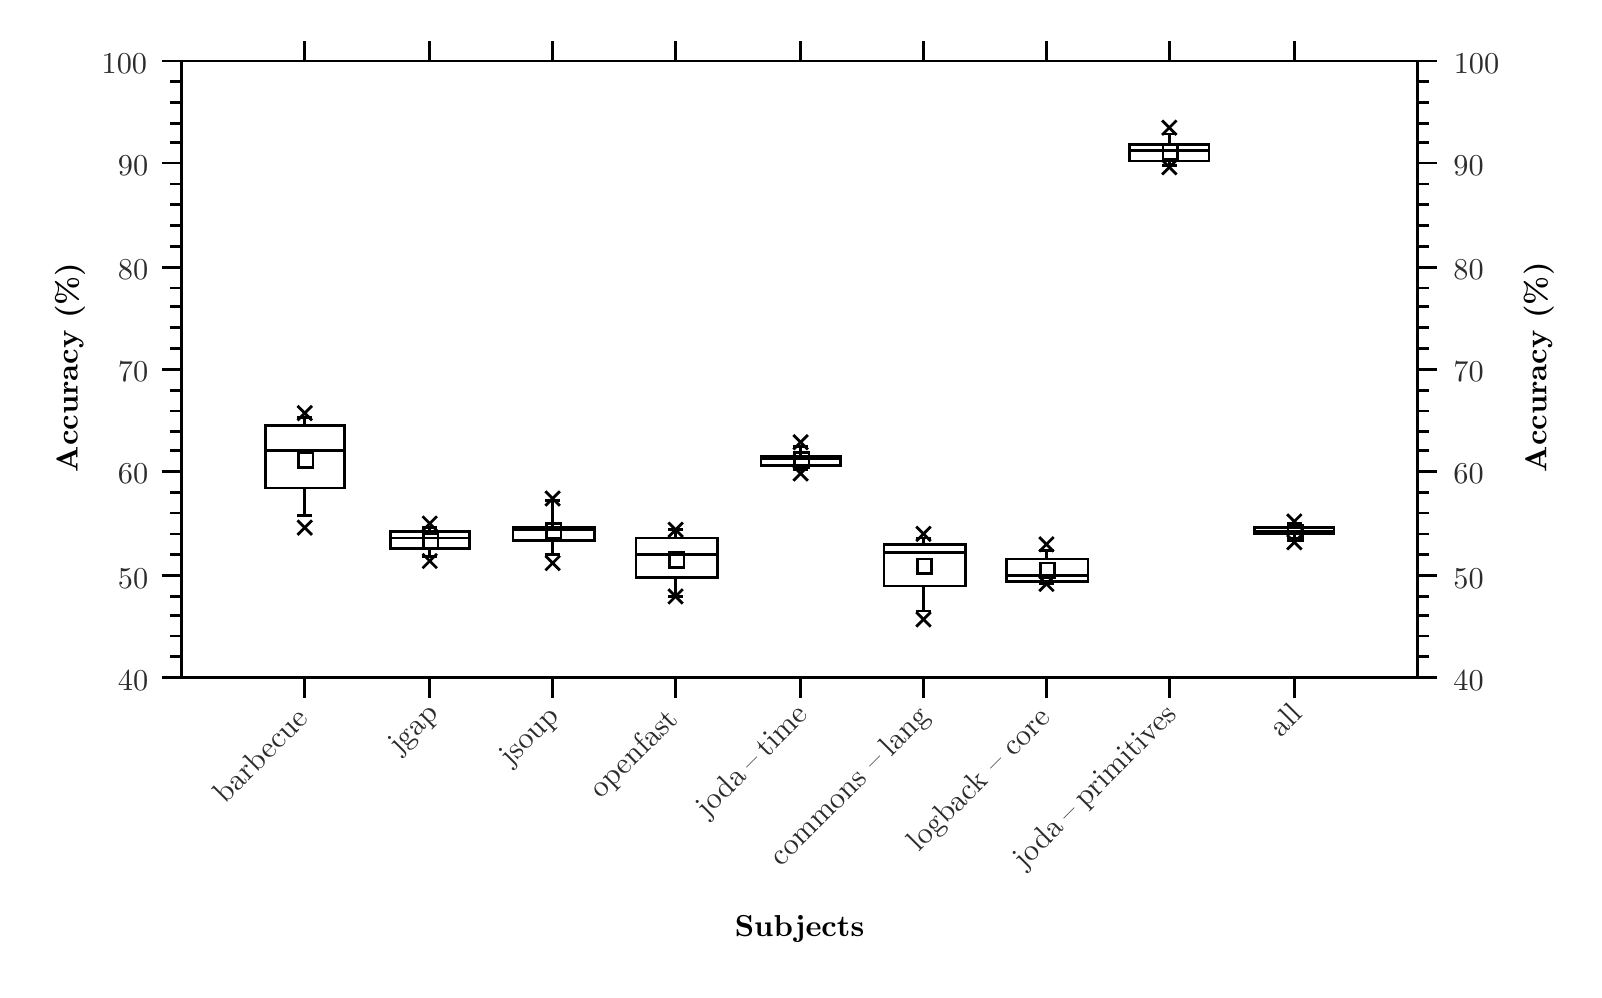
\begin{tikzpicture}{0pt}{0pt}{742pt}{452pt}
	\clip(0pt,452pt) -- (558.587pt,452pt) -- (558.587pt,111.729pt) -- (0pt,111.729pt) -- (0pt,452pt);
\begin{scope}
	\clip(55.7081pt,439.955pt) -- (502.126pt,439.955pt) -- (502.126pt,217.123pt) -- (55.7081pt,217.123pt) -- (55.7081pt,439.955pt);
	\color[rgb]{0,0,0}
	\draw[line width=1pt, line join=miter, line cap=rect](85.8206pt,308.213pt) -- (114.427pt,308.213pt) -- (114.427pt,285.628pt) -- (85.8206pt,285.628pt) -- (85.8206pt,308.213pt);
	\color[rgb]{0,0,0}
	\draw[line width=1pt, line join=miter, line cap=rect](97.8656pt,275.842pt) -- (102.382pt,275.842pt);
	\draw[line width=1pt, line join=miter, line cap=rect](97.8656pt,311.224pt) -- (102.382pt,311.224pt);
	\draw[line width=1pt, line join=miter, line cap=rect](100.124pt,311.224pt) -- (100.124pt,308.213pt);
	\draw[line width=1pt, line join=miter, line cap=rect](100.124pt,275.842pt) -- (100.124pt,285.628pt);
	\draw[line width=1pt, line join=miter, line cap=rect](85.8206pt,299.179pt) -- (114.427pt,299.179pt);
	\draw[line width=1pt, line join=miter, line cap=rect](97.8656pt,273.583pt) -- (102.382pt,269.067pt);
	\draw[line width=1pt, line join=miter, line cap=rect](97.8656pt,269.067pt) -- (102.382pt,273.583pt);
	\draw[line width=1pt, line join=miter, line cap=rect](97.8656pt,314.988pt) -- (102.382pt,310.471pt);
	\draw[line width=1pt, line join=miter, line cap=rect](97.8656pt,310.471pt) -- (102.382pt,314.988pt);
	\draw[line width=1pt, line join=miter, line cap=rect](97.8656pt,298.426pt) -- (103.135pt,298.426pt) -- (103.135pt,293.157pt) -- (97.8656pt,293.157pt) -- (97.8656pt,298.426pt);
	\draw[line width=1pt, line join=miter, line cap=rect](130.989pt,269.819pt) -- (159.596pt,269.819pt) -- (159.596pt,263.797pt) -- (130.989pt,263.797pt) -- (130.989pt,269.819pt);
	\draw[line width=1pt, line join=miter, line cap=rect](143.034pt,260.786pt) -- (147.551pt,260.786pt);
	\draw[line width=1pt, line join=miter, line cap=rect](143.034pt,271.325pt) -- (147.551pt,271.325pt);
	\draw[line width=1pt, line join=miter, line cap=rect](145.293pt,271.325pt) -- (145.293pt,269.819pt);
	\draw[line width=1pt, line join=miter, line cap=rect](145.293pt,260.786pt) -- (145.293pt,263.797pt);
	\draw[line width=1pt, line join=miter, line cap=rect](130.989pt,267.561pt) -- (159.596pt,267.561pt);
	\draw[line width=1pt, line join=miter, line cap=rect](143.034pt,261.538pt) -- (147.551pt,257.022pt);
	\draw[line width=1pt, line join=miter, line cap=rect](143.034pt,257.022pt) -- (147.551pt,261.538pt);
	\draw[line width=1pt, line join=miter, line cap=rect](143.034pt,275.089pt) -- (147.551pt,270.572pt);
	\draw[line width=1pt, line join=miter, line cap=rect](143.034pt,270.572pt) -- (147.551pt,275.089pt);
	\draw[line width=1pt, line join=miter, line cap=rect](143.034pt,269.067pt) -- (148.304pt,269.067pt) -- (148.304pt,263.797pt) -- (143.034pt,263.797pt) -- (143.034pt,269.067pt);
	\draw[line width=1pt, line join=miter, line cap=rect](175.405pt,271.325pt) -- (204.765pt,271.325pt) -- (204.765pt,266.808pt) -- (175.405pt,266.808pt) -- (175.405pt,271.325pt);
	\draw[line width=1pt, line join=miter, line cap=rect](187.45pt,261.538pt) -- (191.967pt,261.538pt);
	\draw[line width=1pt, line join=miter, line cap=rect](187.45pt,281.112pt) -- (191.967pt,281.112pt);
	\draw[line width=1pt, line join=miter, line cap=rect](189.709pt,281.112pt) -- (189.709pt,271.325pt);
	\draw[line width=1pt, line join=miter, line cap=rect](189.709pt,261.538pt) -- (189.709pt,266.808pt);
	\draw[line width=1pt, line join=miter, line cap=rect](175.405pt,270.572pt) -- (204.012pt,270.572pt);
	\draw[line width=1pt, line join=miter, line cap=rect](187.45pt,260.786pt) -- (191.967pt,256.269pt);
	\draw[line width=1pt, line join=miter, line cap=rect](187.45pt,256.269pt) -- (191.967pt,260.786pt);
	\draw[line width=1pt, line join=miter, line cap=rect](187.45pt,284.123pt) -- (191.967pt,279.606pt);
	\draw[line width=1pt, line join=miter, line cap=rect](187.45pt,279.606pt) -- (191.967pt,284.123pt);
	\draw[line width=1pt, line join=miter, line cap=rect](187.45pt,272.831pt) -- (192.72pt,272.831pt) -- (192.72pt,267.561pt) -- (187.45pt,267.561pt) -- (187.45pt,272.831pt);
	\draw[line width=1pt, line join=miter, line cap=rect](219.821pt,267.561pt) -- (249.181pt,267.561pt) -- (249.181pt,253.257pt) -- (219.821pt,253.257pt) -- (219.821pt,267.561pt);
	\draw[line width=1pt, line join=miter, line cap=rect](231.866pt,246.482pt) -- (236.383pt,246.482pt);
	\draw[line width=1pt, line join=miter, line cap=rect](231.866pt,270.572pt) -- (236.383pt,270.572pt);
	\draw[line width=1pt, line join=miter, line cap=rect](234.125pt,270.572pt) -- (234.125pt,267.561pt);
	\draw[line width=1pt, line join=miter, line cap=rect](234.125pt,246.482pt) -- (234.125pt,253.257pt);
	\draw[line width=1pt, line join=miter, line cap=rect](219.821pt,261.538pt) -- (248.428pt,261.538pt);
	\draw[line width=1pt, line join=miter, line cap=rect](231.866pt,248.741pt) -- (236.383pt,244.224pt);
	\draw[line width=1pt, line join=miter, line cap=rect](231.866pt,244.224pt) -- (236.383pt,248.741pt);
	\draw[line width=1pt, line join=miter, line cap=rect](231.866pt,272.831pt) -- (236.383pt,268.314pt);
	\draw[line width=1pt, line join=miter, line cap=rect](231.866pt,268.314pt) -- (236.383pt,272.831pt);
	\draw[line width=1pt, line join=miter, line cap=rect](231.866pt,262.291pt) -- (237.136pt,262.291pt) -- (237.136pt,257.022pt) -- (231.866pt,257.022pt) -- (231.866pt,262.291pt);
	\draw[line width=1pt, line join=miter, line cap=rect](264.99pt,296.921pt) -- (293.597pt,296.921pt) -- (293.597pt,293.909pt) -- (264.99pt,293.909pt) -- (264.99pt,296.921pt);
	\draw[line width=1pt, line join=miter, line cap=rect](277.035pt,292.404pt) -- (281.552pt,292.404pt);
	\draw[line width=1pt, line join=miter, line cap=rect](277.035pt,300.685pt) -- (281.552pt,300.685pt);
	\draw[line width=1pt, line join=miter, line cap=rect](279.293pt,300.685pt) -- (279.293pt,296.921pt);
	\draw[line width=1pt, line join=miter, line cap=rect](279.293pt,292.404pt) -- (279.293pt,293.909pt);
	\draw[line width=1pt, line join=miter, line cap=rect](264.99pt,296.168pt) -- (293.597pt,296.168pt);
	\draw[line width=1pt, line join=miter, line cap=rect](277.035pt,293.157pt) -- (281.552pt,288.64pt);
	\draw[line width=1pt, line join=miter, line cap=rect](277.035pt,288.64pt) -- (281.552pt,293.157pt);
	\draw[line width=1pt, line join=miter, line cap=rect](277.035pt,304.449pt) -- (281.552pt,299.932pt);
	\draw[line width=1pt, line join=miter, line cap=rect](277.035pt,299.932pt) -- (281.552pt,304.449pt);
	\draw[line width=1pt, line join=miter, line cap=rect](277.035pt,298.426pt) -- (282.305pt,298.426pt) -- (282.305pt,293.157pt) -- (277.035pt,293.157pt) -- (277.035pt,298.426pt);
	\draw[line width=1pt, line join=miter, line cap=rect](309.406pt,265.303pt) -- (338.766pt,265.303pt) -- (338.766pt,250.246pt) -- (309.406pt,250.246pt) -- (309.406pt,265.303pt);
	\draw[line width=1pt, line join=miter, line cap=rect](321.451pt,241.213pt) -- (325.968pt,241.213pt);
	\draw[line width=1pt, line join=miter, line cap=rect](321.451pt,267.561pt) -- (325.968pt,267.561pt);
	\draw[line width=1pt, line join=miter, line cap=rect](323.709pt,267.561pt) -- (323.709pt,265.303pt);
	\draw[line width=1pt, line join=miter, line cap=rect](323.709pt,241.213pt) -- (323.709pt,250.246pt);
	\draw[line width=1pt, line join=miter, line cap=rect](309.406pt,262.291pt) -- (338.013pt,262.291pt);
	\draw[line width=1pt, line join=miter, line cap=rect](321.451pt,240.46pt) -- (325.968pt,235.943pt);
	\draw[line width=1pt, line join=miter, line cap=rect](321.451pt,235.943pt) -- (325.968pt,240.46pt);
	\draw[line width=1pt, line join=miter, line cap=rect](321.451pt,271.325pt) -- (325.968pt,266.808pt);
	\draw[line width=1pt, line join=miter, line cap=rect](321.451pt,266.808pt) -- (325.968pt,271.325pt);
	\draw[line width=1pt, line join=miter, line cap=rect](321.451pt,260.033pt) -- (326.721pt,260.033pt) -- (326.721pt,254.763pt) -- (321.451pt,254.763pt) -- (321.451pt,260.033pt);
	\draw[line width=1pt, line join=miter, line cap=rect](353.822pt,260.033pt) -- (383.182pt,260.033pt) -- (383.182pt,251.752pt) -- (353.822pt,251.752pt) -- (353.822pt,260.033pt);
	\draw[line width=1pt, line join=miter, line cap=rect](365.867pt,250.999pt) -- (370.384pt,250.999pt);
	\draw[line width=1pt, line join=miter, line cap=rect](365.867pt,263.044pt) -- (370.384pt,263.044pt);
	\draw[line width=1pt, line join=miter, line cap=rect](368.125pt,263.044pt) -- (368.125pt,260.033pt);
	\draw[line width=1pt, line join=miter, line cap=rect](368.125pt,250.999pt) -- (368.125pt,251.752pt);
	\draw[line width=1pt, line join=miter, line cap=rect](353.822pt,254.01pt) -- (382.429pt,254.01pt);
	\draw[line width=1pt, line join=miter, line cap=rect](365.867pt,253.257pt) -- (370.384pt,248.741pt);
	\draw[line width=1pt, line join=miter, line cap=rect](365.867pt,248.741pt) -- (370.384pt,253.257pt);
	\draw[line width=1pt, line join=miter, line cap=rect](365.867pt,267.561pt) -- (370.384pt,263.044pt);
	\draw[line width=1pt, line join=miter, line cap=rect](365.867pt,263.044pt) -- (370.384pt,267.561pt);
	\draw[line width=1pt, line join=miter, line cap=rect](365.867pt,258.527pt) -- (371.137pt,258.527pt) -- (371.137pt,253.257pt) -- (365.867pt,253.257pt) -- (365.867pt,258.527pt);
	\draw[line width=1pt, line join=miter, line cap=rect](398.238pt,409.842pt) -- (426.845pt,409.842pt) -- (426.845pt,403.82pt) -- (398.238pt,403.82pt) -- (398.238pt,409.842pt);
	\draw[line width=1pt, line join=miter, line cap=rect](410.283pt,402.314pt) -- (414.8pt,402.314pt);
	\draw[line width=1pt, line join=miter, line cap=rect](410.283pt,413.607pt) -- (414.8pt,413.607pt);
	\draw[line width=1pt, line join=miter, line cap=rect](412.541pt,413.607pt) -- (412.541pt,409.842pt);
	\draw[line width=1pt, line join=miter, line cap=rect](412.541pt,402.314pt) -- (412.541pt,403.82pt);
	\draw[line width=1pt, line join=miter, line cap=rect](398.238pt,407.584pt) -- (426.845pt,407.584pt);
	\draw[line width=1pt, line join=miter, line cap=rect](410.283pt,403.82pt) -- (414.8pt,399.303pt);
	\draw[line width=1pt, line join=miter, line cap=rect](410.283pt,399.303pt) -- (414.8pt,403.82pt);
	\draw[line width=1pt, line join=miter, line cap=rect](410.283pt,418.123pt) -- (414.8pt,413.607pt);
	\draw[line width=1pt, line join=miter, line cap=rect](410.283pt,413.607pt) -- (414.8pt,418.123pt);
	\draw[line width=1pt, line join=miter, line cap=rect](410.283pt,409.842pt) -- (415.553pt,409.842pt) -- (415.553pt,404.573pt) -- (410.283pt,404.573pt) -- (410.283pt,409.842pt);
	\draw[line width=1pt, line join=miter, line cap=rect](443.407pt,271.325pt) -- (472.013pt,271.325pt) -- (472.013pt,269.067pt) -- (443.407pt,269.067pt) -- (443.407pt,271.325pt);
	\draw[line width=1pt, line join=miter, line cap=rect](455.452pt,267.561pt) -- (459.968pt,267.561pt);
	\draw[line width=1pt, line join=miter, line cap=rect](455.452pt,272.831pt) -- (459.968pt,272.831pt);
	\draw[line width=1pt, line join=miter, line cap=rect](457.71pt,272.831pt) -- (457.71pt,271.325pt);
	\draw[line width=1pt, line join=miter, line cap=rect](457.71pt,267.561pt) -- (457.71pt,269.067pt);
	\draw[line width=1pt, line join=miter, line cap=rect](443.407pt,269.819pt) -- (472.013pt,269.819pt);
	\draw[line width=1pt, line join=miter, line cap=rect](455.452pt,268.314pt) -- (459.968pt,263.797pt);
	\draw[line width=1pt, line join=miter, line cap=rect](455.452pt,263.797pt) -- (459.968pt,268.314pt);
	\draw[line width=1pt, line join=miter, line cap=rect](455.452pt,275.842pt) -- (459.968pt,271.325pt);
	\draw[line width=1pt, line join=miter, line cap=rect](455.452pt,271.325pt) -- (459.968pt,275.842pt);
	\draw[line width=1pt, line join=miter, line cap=rect](455.452pt,272.078pt) -- (460.721pt,272.078pt) -- (460.721pt,266.808pt) -- (455.452pt,266.808pt) -- (455.452pt,272.078pt);
\end{scope}
\begin{scope}
	\color[rgb]{0,0,0}
	\pgftext[center, base, at={\pgfpoint{18.0675pt}{329.292pt}},rotate=90]{\fontsize{11}{0}\selectfont{\textbf{Accuracy (\%)}}}
	\color[rgb]{0.172549,0.172549,0.172549}
	\pgftext[center, base, at={\pgfpoint{38.1111pt}{212.606pt}}]{\fontsize{11}{0}\selectfont{40}}
	\pgftext[center, base, at={\pgfpoint{38.1111pt}{249.493pt}}]{\fontsize{11}{0}\selectfont{50}}
	\pgftext[center, base, at={\pgfpoint{38.1111pt}{287.134pt}}]{\fontsize{11}{0}\selectfont{60}}
	\pgftext[center, base, at={\pgfpoint{38.1111pt}{324.022pt}}]{\fontsize{11}{0}\selectfont{70}}
	\pgftext[center, base, at={\pgfpoint{38.1111pt}{360.91pt}}]{\fontsize{11}{0}\selectfont{80}}
	\pgftext[center, base, at={\pgfpoint{38.1111pt}{398.55pt}}]{\fontsize{11}{0}\selectfont{90}}
	\pgftext[center, base, at={\pgfpoint{34.9587pt}{435.438pt}}]{\fontsize{11}{0}\selectfont{100}}
	\color[rgb]{0,0,0}
	\draw[line width=1pt, line join=bevel, line cap=rect](55.7081pt,224.651pt) -- (51.9441pt,224.651pt);
	\draw[line width=1pt, line join=bevel, line cap=rect](55.7081pt,232.179pt) -- (51.9441pt,232.179pt);
	\draw[line width=1pt, line join=bevel, line cap=rect](55.7081pt,239.707pt) -- (51.9441pt,239.707pt);
	\draw[line width=1pt, line join=bevel, line cap=rect](55.7081pt,246.482pt) -- (51.9441pt,246.482pt);
	\draw[line width=1pt, line join=bevel, line cap=rect](55.7081pt,261.538pt) -- (51.9441pt,261.538pt);
	\draw[line width=1pt, line join=bevel, line cap=rect](55.7081pt,269.067pt) -- (51.9441pt,269.067pt);
	\draw[line width=1pt, line join=bevel, line cap=rect](55.7081pt,276.595pt) -- (51.9441pt,276.595pt);
	\draw[line width=1pt, line join=bevel, line cap=rect](55.7081pt,284.123pt) -- (51.9441pt,284.123pt);
	\draw[line width=1pt, line join=bevel, line cap=rect](55.7081pt,299.179pt) -- (51.9441pt,299.179pt);
	\draw[line width=1pt, line join=bevel, line cap=rect](55.7081pt,305.954pt) -- (51.9441pt,305.954pt);
	\draw[line width=1pt, line join=bevel, line cap=rect](55.7081pt,313.482pt) -- (51.9441pt,313.482pt);
	\draw[line width=1pt, line join=bevel, line cap=rect](55.7081pt,321.011pt) -- (51.9441pt,321.011pt);
	\draw[line width=1pt, line join=bevel, line cap=rect](55.7081pt,336.067pt) -- (51.9441pt,336.067pt);
	\draw[line width=1pt, line join=bevel, line cap=rect](55.7081pt,343.595pt) -- (51.9441pt,343.595pt);
	\draw[line width=1pt, line join=bevel, line cap=rect](55.7081pt,351.123pt) -- (51.9441pt,351.123pt);
	\draw[line width=1pt, line join=bevel, line cap=rect](55.7081pt,357.898pt) -- (51.9441pt,357.898pt);
	\draw[line width=1pt, line join=bevel, line cap=rect](55.7081pt,372.955pt) -- (51.9441pt,372.955pt);
	\draw[line width=1pt, line join=bevel, line cap=rect](55.7081pt,380.483pt) -- (51.9441pt,380.483pt);
	\draw[line width=1pt, line join=bevel, line cap=rect](55.7081pt,388.011pt) -- (51.9441pt,388.011pt);
	\draw[line width=1pt, line join=bevel, line cap=rect](55.7081pt,395.539pt) -- (51.9441pt,395.539pt);
	\draw[line width=1pt, line join=bevel, line cap=rect](55.7081pt,410.595pt) -- (51.9441pt,410.595pt);
	\draw[line width=1pt, line join=bevel, line cap=rect](55.7081pt,417.371pt) -- (51.9441pt,417.371pt);
	\draw[line width=1pt, line join=bevel, line cap=rect](55.7081pt,424.899pt) -- (51.9441pt,424.899pt);
	\draw[line width=1pt, line join=bevel, line cap=rect](55.7081pt,432.427pt) -- (51.9441pt,432.427pt);
	\draw[line width=1pt, line join=bevel, line cap=rect](55.7081pt,217.123pt) -- (48.9328pt,217.123pt);
	\draw[line width=1pt, line join=bevel, line cap=rect](55.7081pt,254.01pt) -- (48.9328pt,254.01pt);
	\draw[line width=1pt, line join=bevel, line cap=rect](55.7081pt,291.651pt) -- (48.9328pt,291.651pt);
	\draw[line width=1pt, line join=bevel, line cap=rect](55.7081pt,328.539pt) -- (48.9328pt,328.539pt);
	\draw[line width=1pt, line join=bevel, line cap=rect](55.7081pt,365.427pt) -- (48.9328pt,365.427pt);
	\draw[line width=1pt, line join=bevel, line cap=rect](55.7081pt,403.067pt) -- (48.9328pt,403.067pt);
	\draw[line width=1pt, line join=bevel, line cap=rect](55.7081pt,439.955pt) -- (48.9328pt,439.955pt);
	\draw[line width=1pt, line join=bevel, line cap=rect](55.7081pt,439.955pt) -- (55.7081pt,217.123pt);
	\pgftext[center, base, at={\pgfpoint{548.8pt}{329.292pt}},rotate=90]{\fontsize{11}{0}\selectfont{\textbf{Accuracy (\%)}}}
	\color[rgb]{0.172549,0.172549,0.172549}
	\pgftext[center, base, at={\pgfpoint{520.664pt}{212.606pt}}]{\fontsize{11}{0}\selectfont{40}}
	\pgftext[center, base, at={\pgfpoint{520.664pt}{249.493pt}}]{\fontsize{11}{0}\selectfont{50}}
	\pgftext[center, base, at={\pgfpoint{520.664pt}{287.134pt}}]{\fontsize{11}{0}\selectfont{60}}
	\pgftext[center, base, at={\pgfpoint{520.664pt}{324.022pt}}]{\fontsize{11}{0}\selectfont{70}}
	\pgftext[center, base, at={\pgfpoint{520.664pt}{360.91pt}}]{\fontsize{11}{0}\selectfont{80}}
	\pgftext[center, base, at={\pgfpoint{520.664pt}{398.55pt}}]{\fontsize{11}{0}\selectfont{90}}
	\pgftext[center, base, at={\pgfpoint{523.534pt}{435.438pt}}]{\fontsize{11}{0}\selectfont{100}}
	\color[rgb]{0,0,0}
	\draw[line width=1pt, line join=bevel, line cap=rect](502.126pt,224.651pt) -- (505.89pt,224.651pt);
	\draw[line width=1pt, line join=bevel, line cap=rect](502.126pt,232.179pt) -- (505.89pt,232.179pt);
	\draw[line width=1pt, line join=bevel, line cap=rect](502.126pt,239.707pt) -- (505.89pt,239.707pt);
	\draw[line width=1pt, line join=bevel, line cap=rect](502.126pt,246.482pt) -- (505.89pt,246.482pt);
	\draw[line width=1pt, line join=bevel, line cap=rect](502.126pt,261.538pt) -- (505.89pt,261.538pt);
	\draw[line width=1pt, line join=bevel, line cap=rect](502.126pt,269.067pt) -- (505.89pt,269.067pt);
	\draw[line width=1pt, line join=bevel, line cap=rect](502.126pt,276.595pt) -- (505.89pt,276.595pt);
	\draw[line width=1pt, line join=bevel, line cap=rect](502.126pt,284.123pt) -- (505.89pt,284.123pt);
	\draw[line width=1pt, line join=bevel, line cap=rect](502.126pt,299.179pt) -- (505.89pt,299.179pt);
	\draw[line width=1pt, line join=bevel, line cap=rect](502.126pt,305.954pt) -- (505.89pt,305.954pt);
	\draw[line width=1pt, line join=bevel, line cap=rect](502.126pt,313.482pt) -- (505.89pt,313.482pt);
	\draw[line width=1pt, line join=bevel, line cap=rect](502.126pt,321.011pt) -- (505.89pt,321.011pt);
	\draw[line width=1pt, line join=bevel, line cap=rect](502.126pt,336.067pt) -- (505.89pt,336.067pt);
	\draw[line width=1pt, line join=bevel, line cap=rect](502.126pt,343.595pt) -- (505.89pt,343.595pt);
	\draw[line width=1pt, line join=bevel, line cap=rect](502.126pt,351.123pt) -- (505.89pt,351.123pt);
	\draw[line width=1pt, line join=bevel, line cap=rect](502.126pt,357.898pt) -- (505.89pt,357.898pt);
	\draw[line width=1pt, line join=bevel, line cap=rect](502.126pt,372.955pt) -- (505.89pt,372.955pt);
	\draw[line width=1pt, line join=bevel, line cap=rect](502.126pt,380.483pt) -- (505.89pt,380.483pt);
	\draw[line width=1pt, line join=bevel, line cap=rect](502.126pt,388.011pt) -- (505.89pt,388.011pt);
	\draw[line width=1pt, line join=bevel, line cap=rect](502.126pt,395.539pt) -- (505.89pt,395.539pt);
	\draw[line width=1pt, line join=bevel, line cap=rect](502.126pt,410.595pt) -- (505.89pt,410.595pt);
	\draw[line width=1pt, line join=bevel, line cap=rect](502.126pt,417.371pt) -- (505.89pt,417.371pt);
	\draw[line width=1pt, line join=bevel, line cap=rect](502.126pt,424.899pt) -- (505.89pt,424.899pt);
	\draw[line width=1pt, line join=bevel, line cap=rect](502.126pt,432.427pt) -- (505.89pt,432.427pt);
	\draw[line width=1pt, line join=bevel, line cap=rect](502.126pt,217.123pt) -- (508.901pt,217.123pt);
	\draw[line width=1pt, line join=bevel, line cap=rect](502.126pt,254.01pt) -- (508.901pt,254.01pt);
	\draw[line width=1pt, line join=bevel, line cap=rect](502.126pt,291.651pt) -- (508.901pt,291.651pt);
	\draw[line width=1pt, line join=bevel, line cap=rect](502.126pt,328.539pt) -- (508.901pt,328.539pt);
	\draw[line width=1pt, line join=bevel, line cap=rect](502.126pt,365.427pt) -- (508.901pt,365.427pt);
	\draw[line width=1pt, line join=bevel, line cap=rect](502.126pt,403.067pt) -- (508.901pt,403.067pt);
	\draw[line width=1pt, line join=bevel, line cap=rect](502.126pt,439.955pt) -- (508.901pt,439.955pt);
	\draw[line width=1pt, line join=bevel, line cap=rect](502.126pt,439.955pt) -- (502.126pt,217.123pt);
	\pgftext[center, base, at={\pgfpoint{278.917pt}{123.774pt}}]{\fontsize{11}{0}\selectfont{\textbf{Subjects}}}
	\color[rgb]{0.172549,0.172549,0.172549}
	\pgftext[center, base, at={\pgfpoint{86.5666pt}{186.638pt}},rotate=45]{\fontsize{11}{0}\selectfont{barbecue}}
	\pgftext[center, base, at={\pgfpoint{141.542pt}{196.444pt}},rotate=45]{\fontsize{11}{0}\selectfont{jgap}}
	\pgftext[center, base, at={\pgfpoint{183.4pt}{193.886pt}},rotate=45]{\fontsize{11}{0}\selectfont{jsoup}}
	\pgftext[center, base, at={\pgfpoint{221.245pt}{187.316pt}},rotate=45]{\fontsize{11}{0}\selectfont{openfast}}
	\pgftext[center, base, at={\pgfpoint{252.794pt}{173.696pt}},rotate=45]{\fontsize{11}{0}\selectfont{joda}}
	\pgftext[center, base, at={\pgfpoint{263.706pt}{184.608pt}},rotate=45]{\fontsize{11}{0}\selectfont{--}}
	\pgftext[center, base, at={\pgfpoint{274.706pt}{195.608pt}},rotate=45]{\fontsize{11}{0}\selectfont{time}}
	\pgftext[center, base, at={\pgfpoint{287.936pt}{164.422pt}},rotate=45]{\fontsize{11}{0}\selectfont{commons}}
	\pgftext[center, base, at={\pgfpoint{308.206pt}{184.692pt}},rotate=45]{\fontsize{11}{0}\selectfont{--}}
	\pgftext[center, base, at={\pgfpoint{319.068pt}{195.554pt}},rotate=45]{\fontsize{11}{0}\selectfont{lang}}
	\pgftext[center, base, at={\pgfpoint{334.627pt}{166.697pt}},rotate=45]{\fontsize{11}{0}\selectfont{logback}}
	\pgftext[center, base, at={\pgfpoint{351.848pt}{183.918pt}},rotate=45]{\fontsize{11}{0}\selectfont{--}}
	\pgftext[center, base, at={\pgfpoint{363.072pt}{195.142pt}},rotate=45]{\fontsize{11}{0}\selectfont{core}}
	\pgftext[center, base, at={\pgfpoint{367.411pt}{155.065pt}},rotate=45]{\fontsize{11}{0}\selectfont{joda}}
	\pgftext[center, base, at={\pgfpoint{378.323pt}{165.977pt}},rotate=45]{\fontsize{11}{0}\selectfont{--}}
	\pgftext[center, base, at={\pgfpoint{398.826pt}{186.48pt}},rotate=45]{\fontsize{11}{0}\selectfont{primitives}}
	\pgftext[center, base, at={\pgfpoint{456.857pt}{199.343pt}},rotate=45]{\fontsize{11}{0}\selectfont{all}}
	\color[rgb]{0,0,0}
	\draw[line width=1pt, line join=bevel, line cap=rect](100.124pt,217.123pt) -- (100.124pt,210.347pt);
	\draw[line width=1pt, line join=bevel, line cap=rect](145.293pt,217.123pt) -- (145.293pt,210.347pt);
	\draw[line width=1pt, line join=bevel, line cap=rect](189.709pt,217.123pt) -- (189.709pt,210.347pt);
	\draw[line width=1pt, line join=bevel, line cap=rect](234.125pt,217.123pt) -- (234.125pt,210.347pt);
	\draw[line width=1pt, line join=bevel, line cap=rect](279.293pt,217.123pt) -- (279.293pt,210.347pt);
	\draw[line width=1pt, line join=bevel, line cap=rect](323.709pt,217.123pt) -- (323.709pt,210.347pt);
	\draw[line width=1pt, line join=bevel, line cap=rect](368.125pt,217.123pt) -- (368.125pt,210.347pt);
	\draw[line width=1pt, line join=bevel, line cap=rect](412.541pt,217.123pt) -- (412.541pt,210.347pt);
	\draw[line width=1pt, line join=bevel, line cap=rect](457.71pt,217.123pt) -- (457.71pt,210.347pt);
	\draw[line width=1pt, line join=bevel, line cap=rect](55.7081pt,217.123pt) -- (502.126pt,217.123pt);
	\draw[line width=1pt, line join=bevel, line cap=rect](100.124pt,439.955pt) -- (100.124pt,446.73pt);
	\draw[line width=1pt, line join=bevel, line cap=rect](145.293pt,439.955pt) -- (145.293pt,446.73pt);
	\draw[line width=1pt, line join=bevel, line cap=rect](189.709pt,439.955pt) -- (189.709pt,446.73pt);
	\draw[line width=1pt, line join=bevel, line cap=rect](234.125pt,439.955pt) -- (234.125pt,446.73pt);
	\draw[line width=1pt, line join=bevel, line cap=rect](279.293pt,439.955pt) -- (279.293pt,446.73pt);
	\draw[line width=1pt, line join=bevel, line cap=rect](323.709pt,439.955pt) -- (323.709pt,446.73pt);
	\draw[line width=1pt, line join=bevel, line cap=rect](368.125pt,439.955pt) -- (368.125pt,446.73pt);
	\draw[line width=1pt, line join=bevel, line cap=rect](412.541pt,439.955pt) -- (412.541pt,446.73pt);
	\draw[line width=1pt, line join=bevel, line cap=rect](457.71pt,439.955pt) -- (457.71pt,446.73pt);
	\draw[line width=1pt, line join=bevel, line cap=rect](55.7081pt,439.955pt) -- (502.126pt,439.955pt);
\end{scope}
\end{tikzpicture}

  \end{adjustbox}
  \caption{Method-level cross-validation accuracy of each subject subject using all feature sets (\ding{172} \ding{173} \ding{174} \ding{175}).}
  \vspace{1mm}
  \footnotesize{\emph{}}
  \vspace{2mm}
  \hrule
  \label{fig:individual_cross_validation_method_1_2_3_4_graph}
\end{figure}

\begin{table}[ht!]
  \centering
  \rowcolors{1}{gray!30}{gray!20}
  \begin{threeparttable}
    \begin{tabular}{|l|r|r|}
      \rowcolor[RGB]{169,196,223}
      \hline & \textbf{Class-Level} & \textbf{Method-Level} \\
      \hline \cellcolor[RGB]{169,196,223} \textbf{logback-core} & 12 & 138 \\
      \hline \cellcolor[RGB]{169,196,223} \textbf{barbecue} & 2 & 36 \\
      \hline \cellcolor[RGB]{169,196,223} \textbf{jgap} & 27 & 197 \\
      \hline \cellcolor[RGB]{169,196,223} \textbf{commons-lang} & 18 & 132 \\
      \hline \cellcolor[RGB]{169,196,223} \textbf{joda-time} & 21 & 259 \\
      \hline \cellcolor[RGB]{169,196,223} \textbf{openfast} & 24 & 73 \\
      \hline \cellcolor[RGB]{169,196,223} \textbf{jsoup} & 13 & 58 \\
      \hline \cellcolor[RGB]{169,196,223} \textbf{joda-primitives} & 1 & 165 \\
      \hline \cellcolor[RGB]{169,196,223} \textbf{all} & 191 & 1104 \\
      \hline
    \end{tabular}
  \end{threeparttable}
  \caption{The amount of data instances for each subject that is used for each category based on undersampling the lowest category to provide balanced data.}
  \vspace{2mm}
  \hrule
  \label{tab:experiments_undersampled_data}
\end{table}

We have looked at the overall cross-validation accuracy using the different feature sets and found that using all feature sets provides the best accuracy. To understand how different projects behave when we apply our technique we considered each subject independently using all the feature sets. Figure~\ref{fig:individual_cross_validation_class_1_2_3_4_graph} illustrates the class-level cross-validations of each subjects with the \emph{all} subject as a comparison. We can see that all but \emph{barbecue} and \emph{joda-primitives} are roughly the same in mean accuracy. All independent subjects have larger variation in their accuracies, this is most likely due to the limited data that each subject provides on its own. Recall that we are undersampling to achieve balanced categories, thus in some situations the amount of data being used can drastically be reduced. In the case of \emph{barbecue} the undersampling only allowed 2 instances of data to be being used for each category, which explains the huge variation that it has. Even worst off \emph{joda-primitives} only has 1 instance for each category, which resulted in a cross-validation accuracy of 0\%. Table~\ref{tab:experiments_undersampled_data} provides the details on the amount of data instances being used with undersampling. Moving on to the method-level source code units presented in Figure~\ref{fig:individual_cross_validation_method_1_2_3_4_graph} we can see that all by \emph{barbecue}, \emph{joda-primitives} and \emph{joda-time} are roughly around the \emph{all} accuracy with slightly larger variations. Again \emph{barbecue} has a low number of data instances being uses which can explain the larger variations in accuracy. With \emph{joda-primitives} we have an usually high cross-validation accuracy present. If we look at the Figure~\ref{fig:mutation_distributions_method_joda-primitives} in Appendix~\ref{app:mutation_score_distributions} we can see that the mutation score distribution is pretty much cleanly separated according to the category ranges (a large number of 100\% and 50\% mutation score methods, with the remaining between these values). It might just be the case that the \emph{joda-primitives}'s data is easier separable to the \gls{svm} thus allowing it achieve high a accuracy. \emph{joda-time} presents a slightly higher cross-validation accuracy then the other subjects, this could be because it has the most data instances available for the \gls{svm} or because it has 48 methods that are very similar (most likely duplicates) as we saw in the covered mutant distribution (see Figure~\ref{fig:covered_mutant_distributions_method_all}). Similar methods would be classified in the same category, thus this could slightly inflate the cross-validation accuracy if this was the case.


\subsection{Prediction}
\label{subsec:experiment_prediction}
By using LIBSVM we want to train a classifier such that it can predict well on \emph{unknown data}. Parameter selection and the training/testing data sets play an important role in making a good classifier. Ultimately, we want to obtain a classifier that is able to \emph{generalize} to new unknown data. In our specific case since we have 8 different subjects (that are most likely not similar to each other in terms of features) in which we want to maximize our performance at predicting unknown data. We used cross-validation in Section~\ref{subsec:experiment_cross_validation} as it mitigates the overfitting problem introduced by training (i.e., a model becomes specifically tuned for the training data set)~\cite{HCL03}. Parameter selection also occurred automatically using a grid search approach to find a set of parameters that maximized the cross-validation accuracy on the training data set.

\begin{table}[ht!]
  \centering
  \rowcolors{1}{gray!30}{gray!20}
  \begin{threeparttable}
    \begin{tabular}{|l|>{\raggedleft\arraybackslash}p{4.25cm}|>{\raggedleft\arraybackslash}p{4.25cm}|}
      \rowcolor[RGB]{169,196,223}
      \hline & \textbf{Class-Level\newline[Low/Medium/High]} & \textbf{Method-Level\newline[Low/Medium/High]} \\
      \hline \cellcolor[RGB]{169,196,223} \textbf{logback-core} & 36/43/0 & 0/3/30 \\
      \hline \cellcolor[RGB]{169,196,223} \textbf{barbecue} & 13/12/0 & 20/15/0 \\
      \hline \cellcolor[RGB]{169,196,223} \textbf{jgap} & 24/19/0 & 26/0/38 \\
      \hline \cellcolor[RGB]{169,196,223} \textbf{commons-lang} & 0/65/5 & 0/186/207 \\
      \hline \cellcolor[RGB]{169,196,223} \textbf{joda-time} & 0/87/44 & 0/296/946 \\
      \hline \cellcolor[RGB]{169,196,223} \textbf{openfast} & 0/33/15 & 0/69/113 \\
      \hline \cellcolor[RGB]{169,196,223} \textbf{jsoup} & 0/18/26 & 0/50/157 \\
      \hline \cellcolor[RGB]{169,196,223} \textbf{joda-primitives} & 0/64/6 & 0/105/75 \\
      \hline \cellcolor[RGB]{169,196,223} \textbf{all\_but\_logback-core} & 48,55,12 & 138/141/168 \\
      \hline \cellcolor[RGB]{169,196,223} \textbf{all\_but\_barbecue} & 15/14/2 & 56/51/36 \\
      \hline \cellcolor[RGB]{169,196,223} \textbf{all\_but\_jgap} & 51/46/27 & 223/197/235 \\
      \hline \cellcolor[RGB]{169,196,223} \textbf{all\_but\_commons-lang} & 18/83/23 & 132/318/339 \\
      \hline \cellcolor[RGB]{169,196,223} \textbf{all\_but\_joda-time} & 21/108/65 & 256/555/1205 \\
      \hline \cellcolor[RGB]{169,196,223} \textbf{all\_but\_openfast} & 24/57/39 & 73/142/186 \\
      \hline \cellcolor[RGB]{169,196,223} \textbf{all\_but\_jsoup} & 13/31/39 & 58/108/215 \\
      \hline \cellcolor[RGB]{169,196,223} \textbf{all\_but\_joda-primitives} & 1/65/7 & 165/270/240 \\
      \hline
    \end{tabular}
  \end{threeparttable}
  \caption{The amount of data instances present in each category for each subject's prediction data set after undersampling (if possible) has occurred.}
  \vspace{2mm}
  \hrule
  \label{tab:experiments_remaining_data}
\end{table}

We conducted a number of tests where we use LIBSVM's \emph{easy script} to find the best parameters that maximize cross-validation accuracy and then apply the classifier to unknown data. As we are still using undersampling we conduct each experiment 10 times to determine the prediction accuracy. We also only consider the prediction accuracy on the remaining unknown data (i.e., what is left from the undersampling) of the experimental subject being used, see Table~\ref{tab:experiments_undersampled_data} for these values. This effect is less on method-level source code units as there is more available data instances available.

\begin{figure}[ht!]
  \centering
  \begin{adjustbox}{max size={.95\textwidth}{.95\textheight}}
    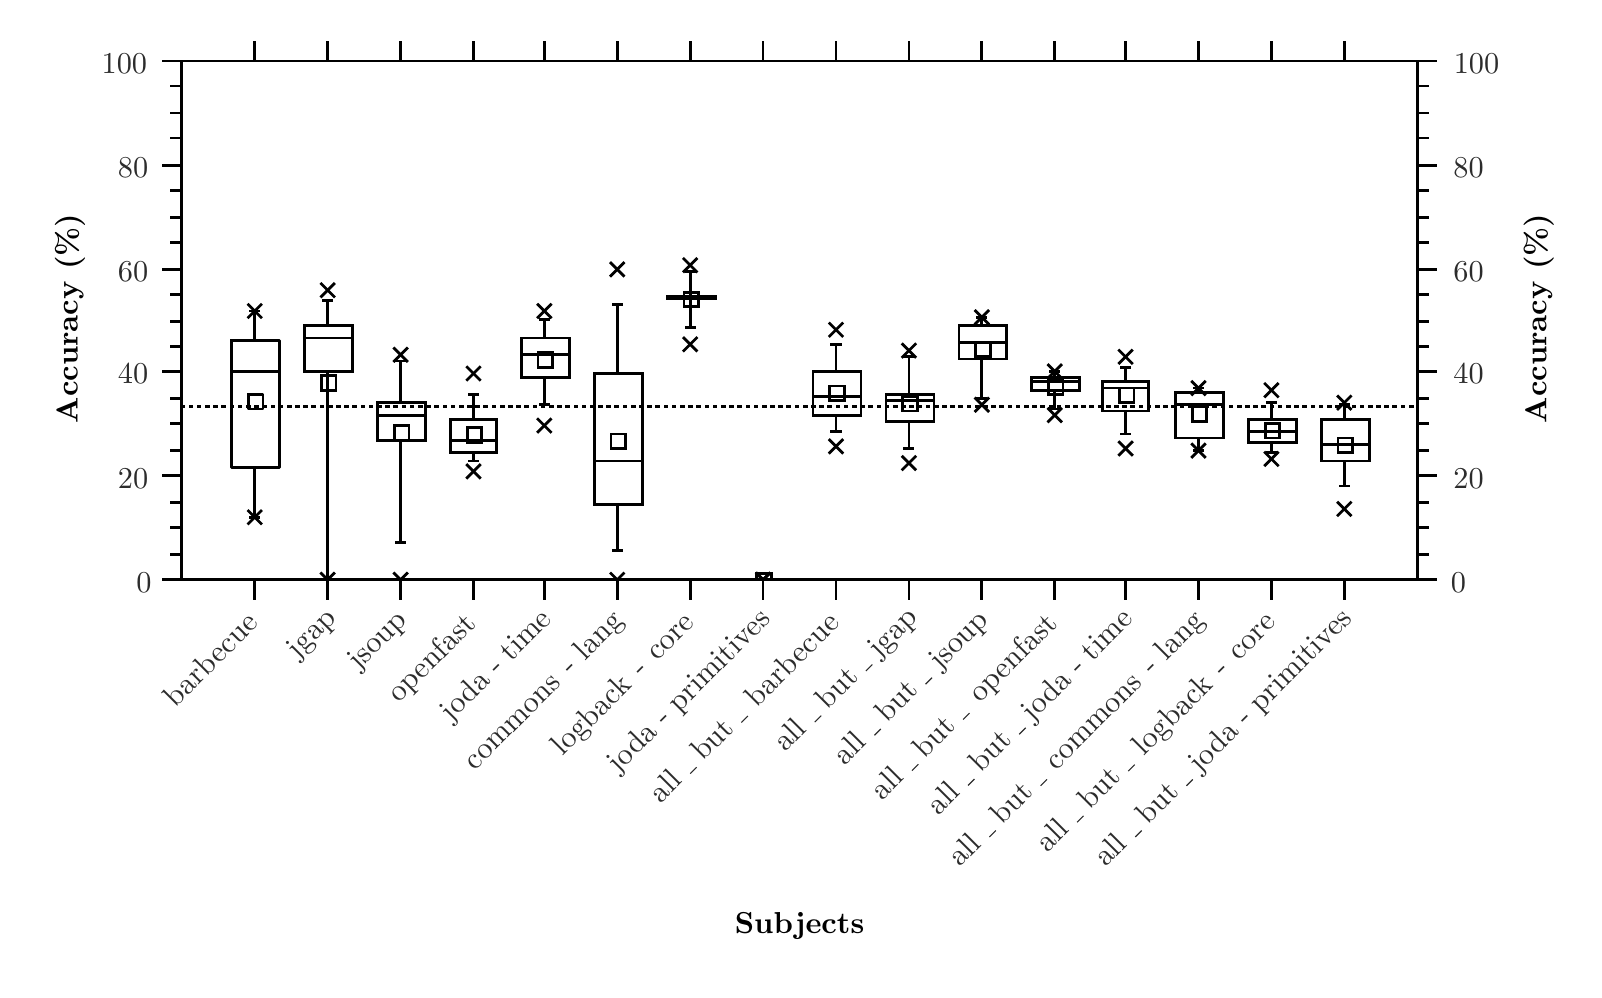
\begin{tikzpicture}{0pt}{0pt}{742pt}{452pt}
	\clip(0pt,452pt) -- (558.587pt,452pt) -- (558.587pt,111.729pt) -- (0pt,111.729pt) -- (0pt,452pt);
\begin{scope}
	\clip(55.7081pt,439.955pt) -- (502.126pt,439.955pt) -- (502.126pt,252.505pt) -- (55.7081pt,252.505pt) -- (55.7081pt,439.955pt);
	\color[rgb]{0,0,0}
	\draw[line width=1pt, line join=bevel, line cap=rect](73.7756pt,339.078pt) -- (91.0903pt,339.078pt) -- (91.0903pt,293.157pt) -- (73.7756pt,293.157pt) -- (73.7756pt,339.078pt);
	\color[rgb]{0,0,0}
	\draw[line width=1pt, line join=bevel, line cap=rect](80.5509pt,275.089pt) -- (83.5622pt,275.089pt);
	\draw[line width=1pt, line join=bevel, line cap=rect](80.5509pt,349.618pt) -- (83.5622pt,349.618pt);
	\draw[line width=1pt, line join=bevel, line cap=rect](82.0566pt,349.618pt) -- (82.0566pt,339.078pt);
	\draw[line width=1pt, line join=bevel, line cap=rect](82.0566pt,275.089pt) -- (82.0566pt,293.157pt);
	\draw[line width=1pt, line join=bevel, line cap=rect](73.7756pt,327.786pt) -- (90.3375pt,327.786pt);
	\draw[line width=1pt, line join=bevel, line cap=rect](79.7981pt,277.347pt) -- (84.315pt,272.831pt);
	\draw[line width=1pt, line join=bevel, line cap=rect](79.7981pt,272.831pt) -- (84.315pt,277.347pt);
	\draw[line width=1pt, line join=bevel, line cap=rect](79.7981pt,351.876pt) -- (84.315pt,347.359pt);
	\draw[line width=1pt, line join=bevel, line cap=rect](79.7981pt,347.359pt) -- (84.315pt,351.876pt);
	\draw[line width=1pt, line join=bevel, line cap=rect](79.7981pt,319.505pt) -- (85.0678pt,319.505pt) -- (85.0678pt,314.235pt) -- (79.7981pt,314.235pt) -- (79.7981pt,319.505pt);
	\draw[line width=1pt, line join=miter, line cap=rect](100.124pt,344.348pt) -- (117.439pt,344.348pt) -- (117.439pt,327.786pt) -- (100.124pt,327.786pt) -- (100.124pt,344.348pt);
	\draw[line width=1pt, line join=miter, line cap=rect](106.899pt,252.505pt) -- (109.911pt,252.505pt);
	\draw[line width=1pt, line join=miter, line cap=rect](106.899pt,353.382pt) -- (109.911pt,353.382pt);
	\draw[line width=1pt, line join=miter, line cap=rect](108.405pt,353.382pt) -- (108.405pt,344.348pt);
	\draw[line width=1pt, line join=miter, line cap=rect](108.405pt,252.505pt) -- (108.405pt,327.786pt);
	\draw[line width=1pt, line join=miter, line cap=rect](100.124pt,339.831pt) -- (116.686pt,339.831pt);
	\draw[line width=1pt, line join=miter, line cap=rect](106.147pt,254.763pt) -- (110.663pt,250.246pt);
	\draw[line width=1pt, line join=miter, line cap=rect](106.147pt,250.246pt) -- (110.663pt,254.763pt);
	\draw[line width=1pt, line join=miter, line cap=rect](106.147pt,359.404pt) -- (110.663pt,354.887pt);
	\draw[line width=1pt, line join=miter, line cap=rect](106.147pt,354.887pt) -- (110.663pt,359.404pt);
	\draw[line width=1pt, line join=miter, line cap=rect](106.147pt,326.28pt) -- (111.416pt,326.28pt) -- (111.416pt,321.011pt) -- (106.147pt,321.011pt) -- (106.147pt,326.28pt);
	\draw[line width=1pt, line join=miter, line cap=rect](126.472pt,316.494pt) -- (143.787pt,316.494pt) -- (143.787pt,302.943pt) -- (126.472pt,302.943pt) -- (126.472pt,316.494pt);
	\draw[line width=1pt, line join=miter, line cap=rect](133.248pt,266.055pt) -- (136.259pt,266.055pt);
	\draw[line width=1pt, line join=miter, line cap=rect](133.248pt,331.55pt) -- (136.259pt,331.55pt);
	\draw[line width=1pt, line join=miter, line cap=rect](134.753pt,331.55pt) -- (134.753pt,316.494pt);
	\draw[line width=1pt, line join=miter, line cap=rect](134.753pt,266.055pt) -- (134.753pt,302.943pt);
	\draw[line width=1pt, line join=miter, line cap=rect](126.472pt,311.977pt) -- (143.034pt,311.977pt);
	\draw[line width=1pt, line join=miter, line cap=rect](132.495pt,254.763pt) -- (137.012pt,250.246pt);
	\draw[line width=1pt, line join=miter, line cap=rect](132.495pt,250.246pt) -- (137.012pt,254.763pt);
	\draw[line width=1pt, line join=miter, line cap=rect](132.495pt,336.067pt) -- (137.012pt,331.55pt);
	\draw[line width=1pt, line join=miter, line cap=rect](132.495pt,331.55pt) -- (137.012pt,336.067pt);
	\draw[line width=1pt, line join=miter, line cap=rect](132.495pt,308.213pt) -- (137.765pt,308.213pt) -- (137.765pt,302.943pt) -- (132.495pt,302.943pt) -- (132.495pt,308.213pt);
	\draw[line width=1pt, line join=miter, line cap=rect](152.821pt,310.471pt) -- (169.383pt,310.471pt) -- (169.383pt,298.426pt) -- (152.821pt,298.426pt) -- (152.821pt,310.471pt);
	\draw[line width=1pt, line join=miter, line cap=rect](159.596pt,295.415pt) -- (162.607pt,295.415pt);
	\draw[line width=1pt, line join=miter, line cap=rect](159.596pt,319.505pt) -- (162.607pt,319.505pt);
	\draw[line width=1pt, line join=miter, line cap=rect](161.102pt,319.505pt) -- (161.102pt,310.471pt);
	\draw[line width=1pt, line join=miter, line cap=rect](161.102pt,295.415pt) -- (161.102pt,298.426pt);
	\draw[line width=1pt, line join=miter, line cap=rect](152.821pt,302.943pt) -- (169.383pt,302.943pt);
	\draw[line width=1pt, line join=miter, line cap=rect](158.843pt,293.909pt) -- (163.36pt,289.393pt);
	\draw[line width=1pt, line join=miter, line cap=rect](158.843pt,289.393pt) -- (163.36pt,293.909pt);
	\draw[line width=1pt, line join=miter, line cap=rect](158.843pt,329.292pt) -- (163.36pt,324.775pt);
	\draw[line width=1pt, line join=miter, line cap=rect](158.843pt,324.775pt) -- (163.36pt,329.292pt);
	\draw[line width=1pt, line join=miter, line cap=rect](158.843pt,307.46pt) -- (164.113pt,307.46pt) -- (164.113pt,302.19pt) -- (158.843pt,302.19pt) -- (158.843pt,307.46pt);
	\draw[line width=1pt, line join=miter, line cap=rect](178.417pt,339.831pt) -- (195.731pt,339.831pt) -- (195.731pt,325.528pt) -- (178.417pt,325.528pt) -- (178.417pt,339.831pt);
	\draw[line width=1pt, line join=miter, line cap=rect](185.192pt,315.741pt) -- (188.203pt,315.741pt);
	\draw[line width=1pt, line join=miter, line cap=rect](185.192pt,346.606pt) -- (188.203pt,346.606pt);
	\draw[line width=1pt, line join=miter, line cap=rect](186.697pt,346.606pt) -- (186.697pt,339.831pt);
	\draw[line width=1pt, line join=miter, line cap=rect](186.697pt,315.741pt) -- (186.697pt,325.528pt);
	\draw[line width=1pt, line join=miter, line cap=rect](178.417pt,333.808pt) -- (194.978pt,333.808pt);
	\draw[line width=1pt, line join=miter, line cap=rect](184.439pt,310.471pt) -- (188.956pt,305.954pt);
	\draw[line width=1pt, line join=miter, line cap=rect](184.439pt,305.954pt) -- (188.956pt,310.471pt);
	\draw[line width=1pt, line join=miter, line cap=rect](184.439pt,351.876pt) -- (188.956pt,347.359pt);
	\draw[line width=1pt, line join=miter, line cap=rect](184.439pt,347.359pt) -- (188.956pt,351.876pt);
	\draw[line width=1pt, line join=miter, line cap=rect](184.439pt,334.561pt) -- (189.709pt,334.561pt) -- (189.709pt,329.292pt) -- (184.439pt,329.292pt) -- (184.439pt,334.561pt);
	\draw[line width=1pt, line join=miter, line cap=rect](204.765pt,327.033pt) -- (222.08pt,327.033pt) -- (222.08pt,279.606pt) -- (204.765pt,279.606pt) -- (204.765pt,327.033pt);
	\draw[line width=1pt, line join=miter, line cap=rect](211.54pt,263.044pt) -- (214.552pt,263.044pt);
	\draw[line width=1pt, line join=miter, line cap=rect](211.54pt,351.876pt) -- (214.552pt,351.876pt);
	\draw[line width=1pt, line join=miter, line cap=rect](213.046pt,351.876pt) -- (213.046pt,327.033pt);
	\draw[line width=1pt, line join=miter, line cap=rect](213.046pt,263.044pt) -- (213.046pt,279.606pt);
	\draw[line width=1pt, line join=miter, line cap=rect](204.765pt,295.415pt) -- (221.327pt,295.415pt);
	\draw[line width=1pt, line join=miter, line cap=rect](210.787pt,254.763pt) -- (215.304pt,250.246pt);
	\draw[line width=1pt, line join=miter, line cap=rect](210.787pt,250.246pt) -- (215.304pt,254.763pt);
	\draw[line width=1pt, line join=miter, line cap=rect](210.787pt,366.932pt) -- (215.304pt,362.415pt);
	\draw[line width=1pt, line join=miter, line cap=rect](210.787pt,362.415pt) -- (215.304pt,366.932pt);
	\draw[line width=1pt, line join=miter, line cap=rect](210.787pt,305.202pt) -- (216.057pt,305.202pt) -- (216.057pt,299.932pt) -- (210.787pt,299.932pt) -- (210.787pt,305.202pt);
	\draw[line width=1pt, line join=miter, line cap=rect](231.113pt,354.887pt) -- (248.428pt,354.887pt) -- (248.428pt,354.134pt) -- (231.113pt,354.134pt) -- (231.113pt,354.887pt);
	\draw[line width=1pt, line join=miter, line cap=rect](237.889pt,343.595pt) -- (240.9pt,343.595pt);
	\draw[line width=1pt, line join=miter, line cap=rect](237.889pt,363.921pt) -- (240.9pt,363.921pt);
	\draw[line width=1pt, line join=miter, line cap=rect](239.394pt,363.921pt) -- (239.394pt,354.887pt);
	\draw[line width=1pt, line join=miter, line cap=rect](239.394pt,343.595pt) -- (239.394pt,354.134pt);
	\draw[line width=1pt, line join=miter, line cap=rect](231.113pt,354.887pt) -- (247.675pt,354.887pt);
	\draw[line width=1pt, line join=miter, line cap=rect](237.136pt,339.831pt) -- (241.653pt,335.314pt);
	\draw[line width=1pt, line join=miter, line cap=rect](237.136pt,335.314pt) -- (241.653pt,339.831pt);
	\draw[line width=1pt, line join=miter, line cap=rect](237.136pt,368.438pt) -- (241.653pt,363.921pt);
	\draw[line width=1pt, line join=miter, line cap=rect](237.136pt,363.921pt) -- (241.653pt,368.438pt);
	\draw[line width=1pt, line join=miter, line cap=rect](237.136pt,356.393pt) -- (242.406pt,356.393pt) -- (242.406pt,351.123pt) -- (237.136pt,351.123pt) -- (237.136pt,356.393pt);
	\draw[line width=1pt, line join=miter, line cap=rect](257.462pt,252.505pt) -- (274.777pt,252.505pt) -- (274.777pt,251.752pt) -- (257.462pt,251.752pt) -- (257.462pt,252.505pt);
	\draw[line width=1pt, line join=miter, line cap=rect](264.237pt,252.505pt) -- (267.248pt,252.505pt);
	\draw[line width=1pt, line join=miter, line cap=rect](264.237pt,252.505pt) -- (267.248pt,252.505pt);
	\draw[line width=1pt, line join=miter, line cap=rect](257.462pt,252.505pt) -- (274.024pt,252.505pt);
	\draw[line width=1pt, line join=miter, line cap=rect](263.484pt,254.763pt) -- (268.001pt,250.246pt);
	\draw[line width=1pt, line join=miter, line cap=rect](263.484pt,250.246pt) -- (268.001pt,254.763pt);
	\draw[line width=1pt, line join=miter, line cap=rect](263.484pt,254.763pt) -- (268.001pt,250.246pt);
	\draw[line width=1pt, line join=miter, line cap=rect](263.484pt,250.246pt) -- (268.001pt,254.763pt);
	\draw[line width=1pt, line join=miter, line cap=rect](263.484pt,254.763pt) -- (268.754pt,254.763pt) -- (268.754pt,249.493pt) -- (263.484pt,249.493pt) -- (263.484pt,254.763pt);
	\draw[line width=1pt, line join=miter, line cap=rect](283.81pt,327.786pt) -- (301.125pt,327.786pt) -- (301.125pt,311.977pt) -- (283.81pt,311.977pt) -- (283.81pt,327.786pt);
	\draw[line width=1pt, line join=miter, line cap=rect](290.586pt,305.954pt) -- (293.597pt,305.954pt);
	\draw[line width=1pt, line join=miter, line cap=rect](290.586pt,337.572pt) -- (293.597pt,337.572pt);
	\draw[line width=1pt, line join=miter, line cap=rect](292.091pt,337.572pt) -- (292.091pt,327.786pt);
	\draw[line width=1pt, line join=miter, line cap=rect](292.091pt,305.954pt) -- (292.091pt,311.977pt);
	\draw[line width=1pt, line join=miter, line cap=rect](283.81pt,318.752pt) -- (300.372pt,318.752pt);
	\draw[line width=1pt, line join=miter, line cap=rect](289.833pt,302.943pt) -- (294.35pt,298.426pt);
	\draw[line width=1pt, line join=miter, line cap=rect](289.833pt,298.426pt) -- (294.35pt,302.943pt);
	\draw[line width=1pt, line join=miter, line cap=rect](289.833pt,345.101pt) -- (294.35pt,340.584pt);
	\draw[line width=1pt, line join=miter, line cap=rect](289.833pt,340.584pt) -- (294.35pt,345.101pt);
	\draw[line width=1pt, line join=miter, line cap=rect](289.833pt,322.516pt) -- (295.103pt,322.516pt) -- (295.103pt,317.247pt) -- (289.833pt,317.247pt) -- (289.833pt,322.516pt);
	\draw[line width=1pt, line join=miter, line cap=rect](310.159pt,319.505pt) -- (327.473pt,319.505pt) -- (327.473pt,309.718pt) -- (310.159pt,309.718pt) -- (310.159pt,319.505pt);
	\draw[line width=1pt, line join=miter, line cap=rect](316.934pt,299.932pt) -- (319.945pt,299.932pt);
	\draw[line width=1pt, line join=miter, line cap=rect](316.934pt,333.056pt) -- (319.945pt,333.056pt);
	\draw[line width=1pt, line join=miter, line cap=rect](318.44pt,333.056pt) -- (318.44pt,319.505pt);
	\draw[line width=1pt, line join=miter, line cap=rect](318.44pt,299.932pt) -- (318.44pt,309.718pt);
	\draw[line width=1pt, line join=miter, line cap=rect](310.159pt,317.247pt) -- (326.721pt,317.247pt);
	\draw[line width=1pt, line join=miter, line cap=rect](316.181pt,296.921pt) -- (320.698pt,292.404pt);
	\draw[line width=1pt, line join=miter, line cap=rect](316.181pt,292.404pt) -- (320.698pt,296.921pt);
	\draw[line width=1pt, line join=miter, line cap=rect](316.181pt,337.572pt) -- (320.698pt,333.056pt);
	\draw[line width=1pt, line join=miter, line cap=rect](316.181pt,333.056pt) -- (320.698pt,337.572pt);
	\draw[line width=1pt, line join=miter, line cap=rect](316.181pt,318.752pt) -- (321.451pt,318.752pt) -- (321.451pt,313.482pt) -- (316.181pt,313.482pt) -- (316.181pt,318.752pt);
	\draw[line width=1pt, line join=miter, line cap=rect](336.507pt,344.348pt) -- (353.822pt,344.348pt) -- (353.822pt,332.303pt) -- (336.507pt,332.303pt) -- (336.507pt,344.348pt);
	\draw[line width=1pt, line join=miter, line cap=rect](343.282pt,317.999pt) -- (346.294pt,317.999pt);
	\draw[line width=1pt, line join=miter, line cap=rect](343.282pt,347.359pt) -- (346.294pt,347.359pt);
	\draw[line width=1pt, line join=miter, line cap=rect](344.788pt,347.359pt) -- (344.788pt,344.348pt);
	\draw[line width=1pt, line join=miter, line cap=rect](344.788pt,317.999pt) -- (344.788pt,332.303pt);
	\draw[line width=1pt, line join=miter, line cap=rect](336.507pt,338.325pt) -- (353.069pt,338.325pt);
	\draw[line width=1pt, line join=miter, line cap=rect](342.53pt,317.999pt) -- (347.047pt,313.482pt);
	\draw[line width=1pt, line join=miter, line cap=rect](342.53pt,313.482pt) -- (347.047pt,317.999pt);
	\draw[line width=1pt, line join=miter, line cap=rect](342.53pt,349.618pt) -- (347.047pt,345.101pt);
	\draw[line width=1pt, line join=miter, line cap=rect](342.53pt,345.101pt) -- (347.047pt,349.618pt);
	\draw[line width=1pt, line join=miter, line cap=rect](342.53pt,338.325pt) -- (347.799pt,338.325pt) -- (347.799pt,333.056pt) -- (342.53pt,333.056pt) -- (342.53pt,338.325pt);
	\draw[line width=1pt, line join=miter, line cap=rect](362.856pt,325.528pt) -- (380.17pt,325.528pt) -- (380.17pt,321.011pt) -- (362.856pt,321.011pt) -- (362.856pt,325.528pt);
	\draw[line width=1pt, line join=miter, line cap=rect](369.631pt,314.235pt) -- (372.642pt,314.235pt);
	\draw[line width=1pt, line join=miter, line cap=rect](369.631pt,327.786pt) -- (372.642pt,327.786pt);
	\draw[line width=1pt, line join=miter, line cap=rect](371.137pt,327.786pt) -- (371.137pt,325.528pt);
	\draw[line width=1pt, line join=miter, line cap=rect](371.137pt,314.235pt) -- (371.137pt,321.011pt);
	\draw[line width=1pt, line join=miter, line cap=rect](362.856pt,324.022pt) -- (379.418pt,324.022pt);
	\draw[line width=1pt, line join=miter, line cap=rect](368.878pt,314.235pt) -- (373.395pt,309.718pt);
	\draw[line width=1pt, line join=miter, line cap=rect](368.878pt,309.718pt) -- (373.395pt,314.235pt);
	\draw[line width=1pt, line join=miter, line cap=rect](368.878pt,330.044pt) -- (373.395pt,325.528pt);
	\draw[line width=1pt, line join=miter, line cap=rect](368.878pt,325.528pt) -- (373.395pt,330.044pt);
	\draw[line width=1pt, line join=miter, line cap=rect](368.878pt,324.775pt) -- (374.148pt,324.775pt) -- (374.148pt,319.505pt) -- (368.878pt,319.505pt) -- (368.878pt,324.775pt);
	\draw[line width=1pt, line join=miter, line cap=rect](388.451pt,324.022pt) -- (405.013pt,324.022pt) -- (405.013pt,313.482pt) -- (388.451pt,313.482pt) -- (388.451pt,324.022pt);
	\draw[line width=1pt, line join=miter, line cap=rect](395.227pt,305.202pt) -- (398.238pt,305.202pt);
	\draw[line width=1pt, line join=miter, line cap=rect](395.227pt,329.292pt) -- (398.238pt,329.292pt);
	\draw[line width=1pt, line join=miter, line cap=rect](396.732pt,329.292pt) -- (396.732pt,324.022pt);
	\draw[line width=1pt, line join=miter, line cap=rect](396.732pt,305.202pt) -- (396.732pt,313.482pt);
	\draw[line width=1pt, line join=miter, line cap=rect](388.451pt,321.763pt) -- (405.013pt,321.763pt);
	\draw[line width=1pt, line join=miter, line cap=rect](394.474pt,302.19pt) -- (398.991pt,297.673pt);
	\draw[line width=1pt, line join=miter, line cap=rect](394.474pt,297.673pt) -- (398.991pt,302.19pt);
	\draw[line width=1pt, line join=miter, line cap=rect](394.474pt,335.314pt) -- (398.991pt,330.797pt);
	\draw[line width=1pt, line join=miter, line cap=rect](394.474pt,330.797pt) -- (398.991pt,335.314pt);
	\draw[line width=1pt, line join=miter, line cap=rect](394.474pt,321.763pt) -- (399.743pt,321.763pt) -- (399.743pt,316.494pt) -- (394.474pt,316.494pt) -- (394.474pt,321.763pt);
	\draw[line width=1pt, line join=miter, line cap=rect](414.8pt,320.258pt) -- (432.114pt,320.258pt) -- (432.114pt,303.696pt) -- (414.8pt,303.696pt) -- (414.8pt,320.258pt);
	\draw[line width=1pt, line join=miter, line cap=rect](421.575pt,299.179pt) -- (424.586pt,299.179pt);
	\draw[line width=1pt, line join=miter, line cap=rect](421.575pt,321.763pt) -- (424.586pt,321.763pt);
	\draw[line width=1pt, line join=miter, line cap=rect](423.081pt,321.763pt) -- (423.081pt,320.258pt);
	\draw[line width=1pt, line join=miter, line cap=rect](423.081pt,299.179pt) -- (423.081pt,303.696pt);
	\draw[line width=1pt, line join=miter, line cap=rect](414.8pt,315.741pt) -- (431.362pt,315.741pt);
	\draw[line width=1pt, line join=miter, line cap=rect](420.822pt,301.438pt) -- (425.339pt,296.921pt);
	\draw[line width=1pt, line join=miter, line cap=rect](420.822pt,296.921pt) -- (425.339pt,301.438pt);
	\draw[line width=1pt, line join=miter, line cap=rect](420.822pt,324.022pt) -- (425.339pt,319.505pt);
	\draw[line width=1pt, line join=miter, line cap=rect](420.822pt,319.505pt) -- (425.339pt,324.022pt);
	\draw[line width=1pt, line join=miter, line cap=rect](420.822pt,314.988pt) -- (426.092pt,314.988pt) -- (426.092pt,309.718pt) -- (420.822pt,309.718pt) -- (420.822pt,314.988pt);
	\draw[line width=1pt, line join=miter, line cap=rect](441.148pt,310.471pt) -- (458.463pt,310.471pt) -- (458.463pt,302.19pt) -- (441.148pt,302.19pt) -- (441.148pt,310.471pt);
	\draw[line width=1pt, line join=miter, line cap=rect](447.923pt,298.426pt) -- (450.935pt,298.426pt);
	\draw[line width=1pt, line join=miter, line cap=rect](447.923pt,316.494pt) -- (450.935pt,316.494pt);
	\draw[line width=1pt, line join=miter, line cap=rect](449.429pt,316.494pt) -- (449.429pt,310.471pt);
	\draw[line width=1pt, line join=miter, line cap=rect](449.429pt,298.426pt) -- (449.429pt,302.19pt);
	\draw[line width=1pt, line join=miter, line cap=rect](441.148pt,305.954pt) -- (457.71pt,305.954pt);
	\draw[line width=1pt, line join=miter, line cap=rect](447.171pt,298.426pt) -- (451.688pt,293.909pt);
	\draw[line width=1pt, line join=miter, line cap=rect](447.171pt,293.909pt) -- (451.688pt,298.426pt);
	\draw[line width=1pt, line join=miter, line cap=rect](447.171pt,323.269pt) -- (451.688pt,318.752pt);
	\draw[line width=1pt, line join=miter, line cap=rect](447.171pt,318.752pt) -- (451.688pt,323.269pt);
	\draw[line width=1pt, line join=miter, line cap=rect](447.171pt,308.966pt) -- (452.44pt,308.966pt) -- (452.44pt,303.696pt) -- (447.171pt,303.696pt) -- (447.171pt,308.966pt);
	\draw[line width=1pt, line join=miter, line cap=rect](467.497pt,310.471pt) -- (484.811pt,310.471pt) -- (484.811pt,295.415pt) -- (467.497pt,295.415pt) -- (467.497pt,310.471pt);
	\draw[line width=1pt, line join=miter, line cap=rect](474.272pt,286.381pt) -- (477.283pt,286.381pt);
	\draw[line width=1pt, line join=miter, line cap=rect](474.272pt,315.741pt) -- (477.283pt,315.741pt);
	\draw[line width=1pt, line join=miter, line cap=rect](475.777pt,315.741pt) -- (475.777pt,310.471pt);
	\draw[line width=1pt, line join=miter, line cap=rect](475.777pt,286.381pt) -- (475.777pt,295.415pt);
	\draw[line width=1pt, line join=miter, line cap=rect](467.497pt,301.438pt) -- (484.058pt,301.438pt);
	\draw[line width=1pt, line join=miter, line cap=rect](473.519pt,280.359pt) -- (478.036pt,275.842pt);
	\draw[line width=1pt, line join=miter, line cap=rect](473.519pt,275.842pt) -- (478.036pt,280.359pt);
	\draw[line width=1pt, line join=miter, line cap=rect](473.519pt,318.752pt) -- (478.036pt,314.235pt);
	\draw[line width=1pt, line join=miter, line cap=rect](473.519pt,314.235pt) -- (478.036pt,318.752pt);
	\draw[line width=1pt, line join=miter, line cap=rect](473.519pt,303.696pt) -- (478.789pt,303.696pt) -- (478.789pt,298.426pt) -- (473.519pt,298.426pt) -- (473.519pt,303.696pt);
	\draw[line width=1pt, dash pattern=on 0.024cm off 0.08cm, dash phase=0pt, line join=miter, line cap=rect](55.7081pt,314.988pt) -- (528.474pt,314.988pt);
\end{scope}
\begin{scope}
	\color[rgb]{0,0,0}
	\pgftext[center, base, at={\pgfpoint{18.0675pt}{346.983pt}},rotate=90]{\fontsize{11}{0}\selectfont{\textbf{Accuracy (\%)}}}
	\color[rgb]{0.172549,0.172549,0.172549}
	\pgftext[center, base, at={\pgfpoint{42.0163pt}{247.988pt}}]{\fontsize{11}{0}\selectfont{0}}
	\pgftext[center, base, at={\pgfpoint{38.1111pt}{285.628pt}}]{\fontsize{11}{0}\selectfont{20}}
	\pgftext[center, base, at={\pgfpoint{38.1111pt}{323.269pt}}]{\fontsize{11}{0}\selectfont{40}}
	\pgftext[center, base, at={\pgfpoint{38.1111pt}{360.157pt}}]{\fontsize{11}{0}\selectfont{60}}
	\pgftext[center, base, at={\pgfpoint{38.1111pt}{397.798pt}}]{\fontsize{11}{0}\selectfont{80}}
	\pgftext[center, base, at={\pgfpoint{34.9587pt}{435.438pt}}]{\fontsize{11}{0}\selectfont{100}}
	\color[rgb]{0,0,0}
	\draw[line width=1pt, line join=bevel, line cap=rect](55.7081pt,261.538pt) -- (51.9441pt,261.538pt);
	\draw[line width=1pt, line join=bevel, line cap=rect](55.7081pt,280.359pt) -- (51.9441pt,280.359pt);
	\draw[line width=1pt, line join=bevel, line cap=rect](55.7081pt,299.179pt) -- (51.9441pt,299.179pt);
	\draw[line width=1pt, line join=bevel, line cap=rect](55.7081pt,317.999pt) -- (51.9441pt,317.999pt);
	\draw[line width=1pt, line join=bevel, line cap=rect](55.7081pt,336.82pt) -- (51.9441pt,336.82pt);
	\draw[line width=1pt, line join=bevel, line cap=rect](55.7081pt,355.64pt) -- (51.9441pt,355.64pt);
	\draw[line width=1pt, line join=bevel, line cap=rect](55.7081pt,374.46pt) -- (51.9441pt,374.46pt);
	\draw[line width=1pt, line join=bevel, line cap=rect](55.7081pt,393.281pt) -- (51.9441pt,393.281pt);
	\draw[line width=1pt, line join=bevel, line cap=rect](55.7081pt,412.101pt) -- (51.9441pt,412.101pt);
	\draw[line width=1pt, line join=bevel, line cap=rect](55.7081pt,430.921pt) -- (51.9441pt,430.921pt);
	\draw[line width=1pt, line join=bevel, line cap=rect](55.7081pt,271.325pt) -- (51.9441pt,271.325pt);
	\draw[line width=1pt, line join=bevel, line cap=rect](55.7081pt,308.966pt) -- (51.9441pt,308.966pt);
	\draw[line width=1pt, line join=bevel, line cap=rect](55.7081pt,345.853pt) -- (51.9441pt,345.853pt);
	\draw[line width=1pt, line join=bevel, line cap=rect](55.7081pt,383.494pt) -- (51.9441pt,383.494pt);
	\draw[line width=1pt, line join=bevel, line cap=rect](55.7081pt,421.135pt) -- (51.9441pt,421.135pt);
	\draw[line width=1pt, line join=bevel, line cap=rect](55.7081pt,252.505pt) -- (48.9328pt,252.505pt);
	\draw[line width=1pt, line join=bevel, line cap=rect](55.7081pt,290.145pt) -- (48.9328pt,290.145pt);
	\draw[line width=1pt, line join=bevel, line cap=rect](55.7081pt,327.786pt) -- (48.9328pt,327.786pt);
	\draw[line width=1pt, line join=bevel, line cap=rect](55.7081pt,364.674pt) -- (48.9328pt,364.674pt);
	\draw[line width=1pt, line join=bevel, line cap=rect](55.7081pt,402.314pt) -- (48.9328pt,402.314pt);
	\draw[line width=1pt, line join=bevel, line cap=rect](55.7081pt,439.955pt) -- (48.9328pt,439.955pt);
	\draw[line width=1pt, line join=bevel, line cap=rect](55.7081pt,439.955pt) -- (55.7081pt,252.505pt);
	\pgftext[center, base, at={\pgfpoint{548.8pt}{346.983pt}},rotate=90]{\fontsize{11}{0}\selectfont{\textbf{Accuracy (\%)}}}
	\color[rgb]{0.172549,0.172549,0.172549}
	\pgftext[center, base, at={\pgfpoint{517.041pt}{247.988pt}}]{\fontsize{11}{0}\selectfont{0}}
	\pgftext[center, base, at={\pgfpoint{520.664pt}{285.628pt}}]{\fontsize{11}{0}\selectfont{20}}
	\pgftext[center, base, at={\pgfpoint{520.664pt}{323.269pt}}]{\fontsize{11}{0}\selectfont{40}}
	\pgftext[center, base, at={\pgfpoint{520.664pt}{360.157pt}}]{\fontsize{11}{0}\selectfont{60}}
	\pgftext[center, base, at={\pgfpoint{520.664pt}{397.798pt}}]{\fontsize{11}{0}\selectfont{80}}
	\pgftext[center, base, at={\pgfpoint{523.534pt}{435.438pt}}]{\fontsize{11}{0}\selectfont{100}}
	\color[rgb]{0,0,0}
	\draw[line width=1pt, line join=bevel, line cap=rect](502.126pt,261.538pt) -- (505.89pt,261.538pt);
	\draw[line width=1pt, line join=bevel, line cap=rect](502.126pt,280.359pt) -- (505.89pt,280.359pt);
	\draw[line width=1pt, line join=bevel, line cap=rect](502.126pt,299.179pt) -- (505.89pt,299.179pt);
	\draw[line width=1pt, line join=bevel, line cap=rect](502.126pt,317.999pt) -- (505.89pt,317.999pt);
	\draw[line width=1pt, line join=bevel, line cap=rect](502.126pt,336.82pt) -- (505.89pt,336.82pt);
	\draw[line width=1pt, line join=bevel, line cap=rect](502.126pt,355.64pt) -- (505.89pt,355.64pt);
	\draw[line width=1pt, line join=bevel, line cap=rect](502.126pt,374.46pt) -- (505.89pt,374.46pt);
	\draw[line width=1pt, line join=bevel, line cap=rect](502.126pt,393.281pt) -- (505.89pt,393.281pt);
	\draw[line width=1pt, line join=bevel, line cap=rect](502.126pt,412.101pt) -- (505.89pt,412.101pt);
	\draw[line width=1pt, line join=bevel, line cap=rect](502.126pt,430.921pt) -- (505.89pt,430.921pt);
	\draw[line width=1pt, line join=bevel, line cap=rect](502.126pt,271.325pt) -- (505.89pt,271.325pt);
	\draw[line width=1pt, line join=bevel, line cap=rect](502.126pt,308.966pt) -- (505.89pt,308.966pt);
	\draw[line width=1pt, line join=bevel, line cap=rect](502.126pt,345.853pt) -- (505.89pt,345.853pt);
	\draw[line width=1pt, line join=bevel, line cap=rect](502.126pt,383.494pt) -- (505.89pt,383.494pt);
	\draw[line width=1pt, line join=bevel, line cap=rect](502.126pt,421.135pt) -- (505.89pt,421.135pt);
	\draw[line width=1pt, line join=bevel, line cap=rect](502.126pt,252.505pt) -- (508.901pt,252.505pt);
	\draw[line width=1pt, line join=bevel, line cap=rect](502.126pt,290.145pt) -- (508.901pt,290.145pt);
	\draw[line width=1pt, line join=bevel, line cap=rect](502.126pt,327.786pt) -- (508.901pt,327.786pt);
	\draw[line width=1pt, line join=bevel, line cap=rect](502.126pt,364.674pt) -- (508.901pt,364.674pt);
	\draw[line width=1pt, line join=bevel, line cap=rect](502.126pt,402.314pt) -- (508.901pt,402.314pt);
	\draw[line width=1pt, line join=bevel, line cap=rect](502.126pt,439.955pt) -- (508.901pt,439.955pt);
	\draw[line width=1pt, line join=bevel, line cap=rect](502.126pt,439.955pt) -- (502.126pt,252.505pt);
	\pgftext[center, base, at={\pgfpoint{278.917pt}{124.527pt}}]{\fontsize{11}{0}\selectfont{\textbf{Subjects}}}
	\color[rgb]{0.172549,0.172549,0.172549}
	\pgftext[center, base, at={\pgfpoint{68.4991pt}{221.267pt}},rotate=45]{\fontsize{11}{0}\selectfont{barbecue}}
	\pgftext[center, base, at={\pgfpoint{104.654pt}{231.073pt}},rotate=45]{\fontsize{11}{0}\selectfont{jgap}}
	\pgftext[center, base, at={\pgfpoint{128.445pt}{228.516pt}},rotate=45]{\fontsize{11}{0}\selectfont{jsoup}}
	\pgftext[center, base, at={\pgfpoint{148.222pt}{221.945pt}},rotate=45]{\fontsize{11}{0}\selectfont{openfast}}
	\pgftext[center, base, at={\pgfpoint{160.198pt}{208.325pt}},rotate=45]{\fontsize{11}{0}\selectfont{joda}}
	\pgftext[center, base, at={\pgfpoint{171.111pt}{219.238pt}},rotate=45]{\fontsize{11}{0}\selectfont{-}}
	\pgftext[center, base, at={\pgfpoint{182.11pt}{230.238pt}},rotate=45]{\fontsize{11}{0}\selectfont{time}}
	\pgftext[center, base, at={\pgfpoint{177.272pt}{199.051pt}},rotate=45]{\fontsize{11}{0}\selectfont{commons}}
	\pgftext[center, base, at={\pgfpoint{197.542pt}{219.321pt}},rotate=45]{\fontsize{11}{0}\selectfont{-}}
	\pgftext[center, base, at={\pgfpoint{208.405pt}{230.184pt}},rotate=45]{\fontsize{11}{0}\selectfont{lang}}
	\pgftext[center, base, at={\pgfpoint{205.896pt}{201.326pt}},rotate=45]{\fontsize{11}{0}\selectfont{logback}}
	\pgftext[center, base, at={\pgfpoint{223.117pt}{218.547pt}},rotate=45]{\fontsize{11}{0}\selectfont{-}}
	\pgftext[center, base, at={\pgfpoint{234.342pt}{229.772pt}},rotate=45]{\fontsize{11}{0}\selectfont{core}}
	\pgftext[center, base, at={\pgfpoint{220.612pt}{189.694pt}},rotate=45]{\fontsize{11}{0}\selectfont{joda}}
	\pgftext[center, base, at={\pgfpoint{231.525pt}{200.607pt}},rotate=45]{\fontsize{11}{0}\selectfont{-}}
	\pgftext[center, base, at={\pgfpoint{252.027pt}{221.109pt}},rotate=45]{\fontsize{11}{0}\selectfont{primitives}}
	\pgftext[center, base, at={\pgfpoint{232.684pt}{175.417pt}},rotate=45]{\fontsize{11}{0}\selectfont{all}}
	\pgftext[center, base, at={\pgfpoint{240.498pt}{183.231pt}},rotate=45]{\fontsize{11}{0}\selectfont{\_}}
	\pgftext[center, base, at={\pgfpoint{249.743pt}{192.476pt}},rotate=45]{\fontsize{11}{0}\selectfont{but}}
	\pgftext[center, base, at={\pgfpoint{258.988pt}{201.721pt}},rotate=45]{\fontsize{11}{0}\selectfont{\_}}
	\pgftext[center, base, at={\pgfpoint{278.584pt}{221.317pt}},rotate=45]{\fontsize{11}{0}\selectfont{barbecue}}
	\pgftext[center, base, at={\pgfpoint{277.663pt}{194.048pt}},rotate=45]{\fontsize{11}{0}\selectfont{all}}
	\pgftext[center, base, at={\pgfpoint{285.478pt}{201.862pt}},rotate=45]{\fontsize{11}{0}\selectfont{\_}}
	\pgftext[center, base, at={\pgfpoint{294.722pt}{211.107pt}},rotate=45]{\fontsize{11}{0}\selectfont{but}}
	\pgftext[center, base, at={\pgfpoint{303.967pt}{220.352pt}},rotate=45]{\fontsize{11}{0}\selectfont{\_}}
	\pgftext[center, base, at={\pgfpoint{314.738pt}{231.123pt}},rotate=45]{\fontsize{11}{0}\selectfont{jgap}}
	\pgftext[center, base, at={\pgfpoint{299.221pt}{189.257pt}},rotate=45]{\fontsize{11}{0}\selectfont{all}}
	\pgftext[center, base, at={\pgfpoint{307.035pt}{197.072pt}},rotate=45]{\fontsize{11}{0}\selectfont{\_}}
	\pgftext[center, base, at={\pgfpoint{316.28pt}{206.317pt}},rotate=45]{\fontsize{11}{0}\selectfont{but}}
	\pgftext[center, base, at={\pgfpoint{325.525pt}{215.561pt}},rotate=45]{\fontsize{11}{0}\selectfont{\_}}
	\pgftext[center, base, at={\pgfpoint{338.529pt}{228.566pt}},rotate=45]{\fontsize{11}{0}\selectfont{jsoup}}
	\pgftext[center, base, at={\pgfpoint{312.794pt}{176.482pt}},rotate=45]{\fontsize{11}{0}\selectfont{all}}
	\pgftext[center, base, at={\pgfpoint{320.608pt}{184.296pt}},rotate=45]{\fontsize{11}{0}\selectfont{\_}}
	\pgftext[center, base, at={\pgfpoint{329.853pt}{193.541pt}},rotate=45]{\fontsize{11}{0}\selectfont{but}}
	\pgftext[center, base, at={\pgfpoint{339.098pt}{202.786pt}},rotate=45]{\fontsize{11}{0}\selectfont{\_}}
	\pgftext[center, base, at={\pgfpoint{358.307pt}{221.995pt}},rotate=45]{\fontsize{11}{0}\selectfont{openfast}}
	\pgftext[center, base, at={\pgfpoint{333.066pt}{171.159pt}},rotate=45]{\fontsize{11}{0}\selectfont{all}}
	\pgftext[center, base, at={\pgfpoint{340.88pt}{178.973pt}},rotate=45]{\fontsize{11}{0}\selectfont{\_}}
	\pgftext[center, base, at={\pgfpoint{350.125pt}{188.218pt}},rotate=45]{\fontsize{11}{0}\selectfont{but}}
	\pgftext[center, base, at={\pgfpoint{359.37pt}{197.463pt}},rotate=45]{\fontsize{11}{0}\selectfont{\_}}
	\pgftext[center, base, at={\pgfpoint{370.283pt}{208.375pt}},rotate=45]{\fontsize{11}{0}\selectfont{joda}}
	\pgftext[center, base, at={\pgfpoint{381.195pt}{219.288pt}},rotate=45]{\fontsize{11}{0}\selectfont{-}}
	\pgftext[center, base, at={\pgfpoint{392.195pt}{230.287pt}},rotate=45]{\fontsize{11}{0}\selectfont{time}}
	\pgftext[center, base, at={\pgfpoint{340.783pt}{152.527pt}},rotate=45]{\fontsize{11}{0}\selectfont{all}}
	\pgftext[center, base, at={\pgfpoint{348.598pt}{160.342pt}},rotate=45]{\fontsize{11}{0}\selectfont{\_}}
	\pgftext[center, base, at={\pgfpoint{357.842pt}{169.587pt}},rotate=45]{\fontsize{11}{0}\selectfont{but}}
	\pgftext[center, base, at={\pgfpoint{367.087pt}{178.831pt}},rotate=45]{\fontsize{11}{0}\selectfont{\_}}
	\pgftext[center, base, at={\pgfpoint{387.357pt}{199.101pt}},rotate=45]{\fontsize{11}{0}\selectfont{commons}}
	\pgftext[center, base, at={\pgfpoint{407.627pt}{219.371pt}},rotate=45]{\fontsize{11}{0}\selectfont{-}}
	\pgftext[center, base, at={\pgfpoint{418.489pt}{230.233pt}},rotate=45]{\fontsize{11}{0}\selectfont{lang}}
	\pgftext[center, base, at={\pgfpoint{372.455pt}{157.851pt}},rotate=45]{\fontsize{11}{0}\selectfont{all}}
	\pgftext[center, base, at={\pgfpoint{380.269pt}{165.665pt}},rotate=45]{\fontsize{11}{0}\selectfont{\_}}
	\pgftext[center, base, at={\pgfpoint{389.514pt}{174.91pt}},rotate=45]{\fontsize{11}{0}\selectfont{but}}
	\pgftext[center, base, at={\pgfpoint{398.759pt}{184.155pt}},rotate=45]{\fontsize{11}{0}\selectfont{\_}}
	\pgftext[center, base, at={\pgfpoint{415.98pt}{201.376pt}},rotate=45]{\fontsize{11}{0}\selectfont{logback}}
	\pgftext[center, base, at={\pgfpoint{433.202pt}{218.597pt}},rotate=45]{\fontsize{11}{0}\selectfont{-}}
	\pgftext[center, base, at={\pgfpoint{444.426pt}{229.822pt}},rotate=45]{\fontsize{11}{0}\selectfont{core}}
	\pgftext[center, base, at={\pgfpoint{393.48pt}{152.527pt}},rotate=45]{\fontsize{11}{0}\selectfont{all}}
	\pgftext[center, base, at={\pgfpoint{401.294pt}{160.342pt}},rotate=45]{\fontsize{11}{0}\selectfont{\_}}
	\pgftext[center, base, at={\pgfpoint{410.539pt}{169.587pt}},rotate=45]{\fontsize{11}{0}\selectfont{but}}
	\pgftext[center, base, at={\pgfpoint{419.784pt}{178.831pt}},rotate=45]{\fontsize{11}{0}\selectfont{\_}}
	\pgftext[center, base, at={\pgfpoint{430.697pt}{189.744pt}},rotate=45]{\fontsize{11}{0}\selectfont{joda}}
	\pgftext[center, base, at={\pgfpoint{441.609pt}{200.656pt}},rotate=45]{\fontsize{11}{0}\selectfont{-}}
	\pgftext[center, base, at={\pgfpoint{462.112pt}{221.159pt}},rotate=45]{\fontsize{11}{0}\selectfont{primitives}}
	\color[rgb]{0,0,0}
	\draw[line width=1pt, line join=bevel, line cap=rect](82.0566pt,252.505pt) -- (82.0566pt,245.729pt);
	\draw[line width=1pt, line join=bevel, line cap=rect](108.405pt,252.505pt) -- (108.405pt,245.729pt);
	\draw[line width=1pt, line join=bevel, line cap=rect](134.753pt,252.505pt) -- (134.753pt,245.729pt);
	\draw[line width=1pt, line join=bevel, line cap=rect](161.102pt,252.505pt) -- (161.102pt,245.729pt);
	\draw[line width=1pt, line join=bevel, line cap=rect](186.697pt,252.505pt) -- (186.697pt,245.729pt);
	\draw[line width=1pt, line join=bevel, line cap=rect](213.046pt,252.505pt) -- (213.046pt,245.729pt);
	\draw[line width=1pt, line join=bevel, line cap=rect](239.394pt,252.505pt) -- (239.394pt,245.729pt);
	\draw[line width=1pt, line join=bevel, line cap=rect](265.743pt,252.505pt) -- (265.743pt,245.729pt);
	\draw[line width=1pt, line join=bevel, line cap=rect](292.091pt,252.505pt) -- (292.091pt,245.729pt);
	\draw[line width=1pt, line join=bevel, line cap=rect](318.44pt,252.505pt) -- (318.44pt,245.729pt);
	\draw[line width=1pt, line join=bevel, line cap=rect](344.788pt,252.505pt) -- (344.788pt,245.729pt);
	\draw[line width=1pt, line join=bevel, line cap=rect](371.137pt,252.505pt) -- (371.137pt,245.729pt);
	\draw[line width=1pt, line join=bevel, line cap=rect](396.732pt,252.505pt) -- (396.732pt,245.729pt);
	\draw[line width=1pt, line join=bevel, line cap=rect](423.081pt,252.505pt) -- (423.081pt,245.729pt);
	\draw[line width=1pt, line join=bevel, line cap=rect](449.429pt,252.505pt) -- (449.429pt,245.729pt);
	\draw[line width=1pt, line join=bevel, line cap=rect](475.777pt,252.505pt) -- (475.777pt,245.729pt);
	\draw[line width=1pt, line join=bevel, line cap=rect](55.7081pt,252.505pt) -- (502.126pt,252.505pt);
	\draw[line width=1pt, line join=bevel, line cap=rect](82.0566pt,439.955pt) -- (82.0566pt,446.73pt);
	\draw[line width=1pt, line join=bevel, line cap=rect](108.405pt,439.955pt) -- (108.405pt,446.73pt);
	\draw[line width=1pt, line join=bevel, line cap=rect](134.753pt,439.955pt) -- (134.753pt,446.73pt);
	\draw[line width=1pt, line join=bevel, line cap=rect](161.102pt,439.955pt) -- (161.102pt,446.73pt);
	\draw[line width=1pt, line join=bevel, line cap=rect](186.697pt,439.955pt) -- (186.697pt,446.73pt);
	\draw[line width=1pt, line join=bevel, line cap=rect](213.046pt,439.955pt) -- (213.046pt,446.73pt);
	\draw[line width=1pt, line join=bevel, line cap=rect](239.394pt,439.955pt) -- (239.394pt,446.73pt);
	\draw[line width=1pt, line join=bevel, line cap=rect](265.743pt,439.955pt) -- (265.743pt,446.73pt);
	\draw[line width=1pt, line join=bevel, line cap=rect](292.091pt,439.955pt) -- (292.091pt,446.73pt);
	\draw[line width=1pt, line join=bevel, line cap=rect](318.44pt,439.955pt) -- (318.44pt,446.73pt);
	\draw[line width=1pt, line join=bevel, line cap=rect](344.788pt,439.955pt) -- (344.788pt,446.73pt);
	\draw[line width=1pt, line join=bevel, line cap=rect](371.137pt,439.955pt) -- (371.137pt,446.73pt);
	\draw[line width=1pt, line join=bevel, line cap=rect](396.732pt,439.955pt) -- (396.732pt,446.73pt);
	\draw[line width=1pt, line join=bevel, line cap=rect](423.081pt,439.955pt) -- (423.081pt,446.73pt);
	\draw[line width=1pt, line join=bevel, line cap=rect](449.429pt,439.955pt) -- (449.429pt,446.73pt);
	\draw[line width=1pt, line join=bevel, line cap=rect](475.777pt,439.955pt) -- (475.777pt,446.73pt);
	\draw[line width=1pt, line join=bevel, line cap=rect](55.7081pt,439.955pt) -- (502.126pt,439.955pt);
\end{scope}
\end{tikzpicture}

  \end{adjustbox}
  \caption{Class-level training and prediction accuracy over the 8 subjects and sets of \emph{all\_but\_<subject>}.}
  \vspace{2mm}
  \hrule
  \label{fig:prediction_class_graph}
\end{figure}

\begin{figure}[ht!]
  \centering
  \begin{adjustbox}{max size={.95\textwidth}{.95\textheight}}
    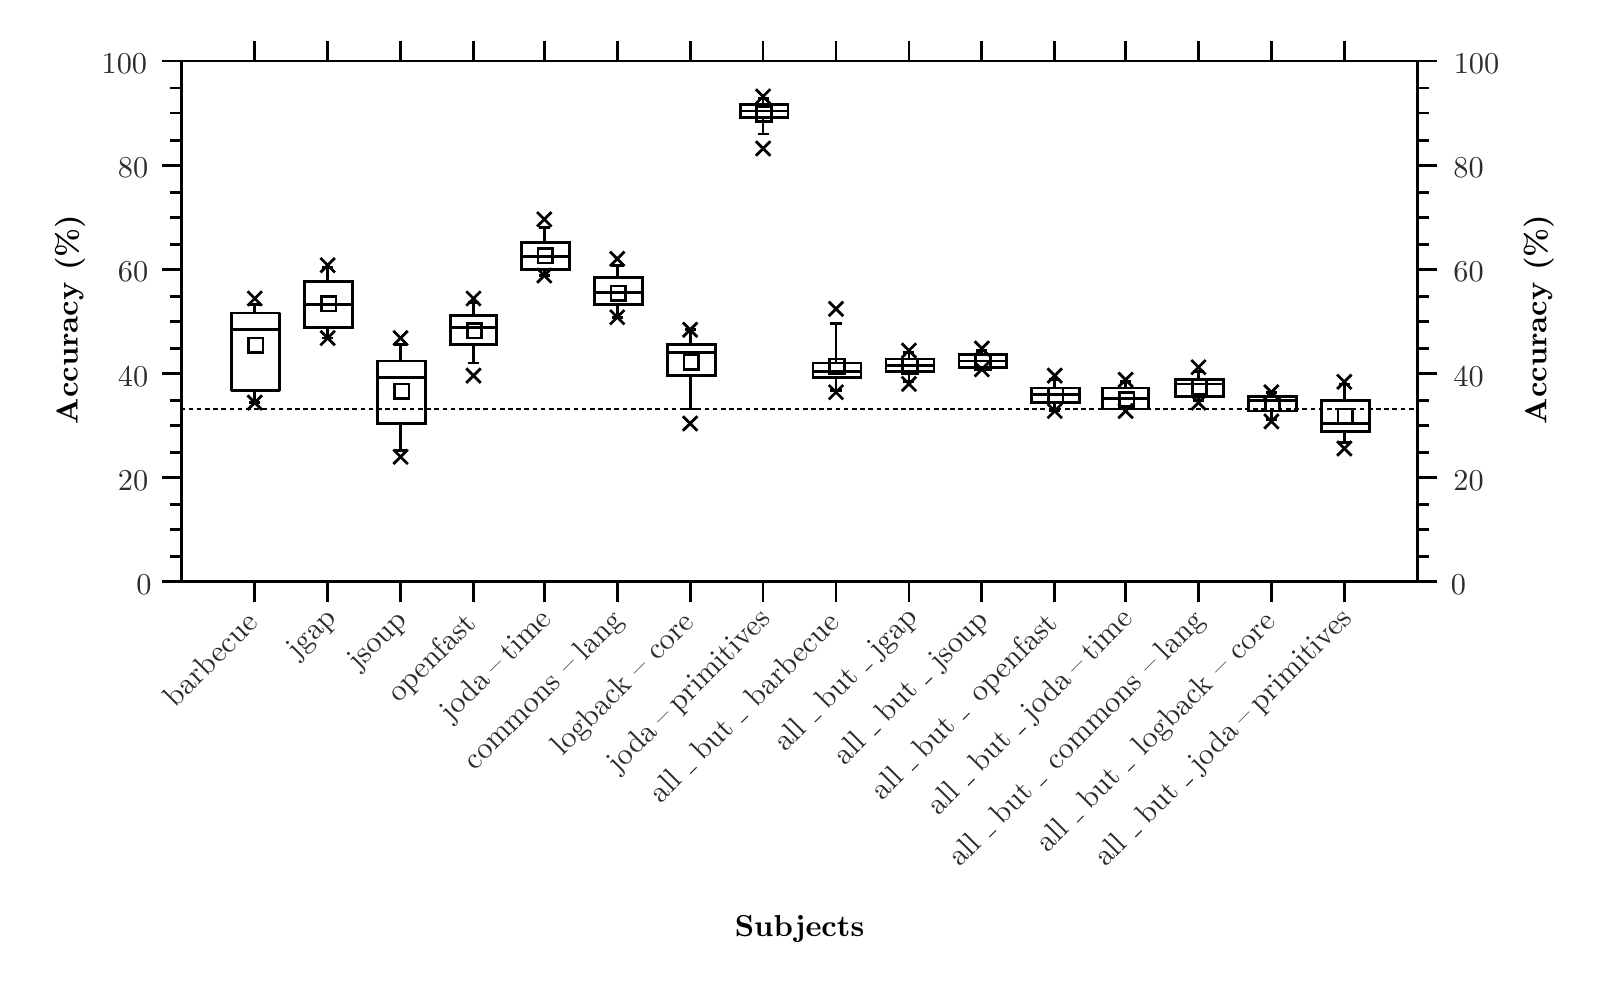
\begin{tikzpicture}{0pt}{0pt}{742pt}{452pt}
	\clip(0pt,452pt) -- (558.587pt,452pt) -- (558.587pt,111.729pt) -- (0pt,111.729pt) -- (0pt,452pt);
\begin{scope}
	\clip(55.7081pt,439.955pt) -- (502.126pt,439.955pt) -- (502.126pt,251.752pt) -- (55.7081pt,251.752pt) -- (55.7081pt,439.955pt);
	\color[rgb]{0,0,0}
	\draw[line width=1pt, line join=bevel, line cap=rect](73.7756pt,348.865pt) -- (91.0903pt,348.865pt) -- (91.0903pt,321.011pt) -- (73.7756pt,321.011pt) -- (73.7756pt,348.865pt);
	\color[rgb]{0,0,0}
	\draw[line width=1pt, line join=bevel, line cap=rect](80.5509pt,316.494pt) -- (83.5622pt,316.494pt);
	\draw[line width=1pt, line join=bevel, line cap=rect](80.5509pt,351.876pt) -- (83.5622pt,351.876pt);
	\draw[line width=1pt, line join=bevel, line cap=rect](82.0566pt,351.876pt) -- (82.0566pt,348.865pt);
	\draw[line width=1pt, line join=bevel, line cap=rect](82.0566pt,316.494pt) -- (82.0566pt,321.011pt);
	\draw[line width=1pt, line join=bevel, line cap=rect](73.7756pt,342.842pt) -- (90.3375pt,342.842pt);
	\draw[line width=1pt, line join=miter, line cap=rect](79.7981pt,318.752pt) -- (84.315pt,314.235pt);
	\draw[line width=1pt, line join=miter, line cap=rect](79.7981pt,314.235pt) -- (84.315pt,318.752pt);
	\draw[line width=1pt, line join=miter, line cap=rect](79.7981pt,356.393pt) -- (84.315pt,351.876pt);
	\draw[line width=1pt, line join=miter, line cap=rect](79.7981pt,351.876pt) -- (84.315pt,356.393pt);
	\draw[line width=1pt, line join=miter, line cap=rect](79.7981pt,339.831pt) -- (85.0678pt,339.831pt) -- (85.0678pt,334.561pt) -- (79.7981pt,334.561pt) -- (79.7981pt,339.831pt);
	\draw[line width=1pt, line join=miter, line cap=rect](100.124pt,360.157pt) -- (117.439pt,360.157pt) -- (117.439pt,343.595pt) -- (100.124pt,343.595pt) -- (100.124pt,360.157pt);
	\draw[line width=1pt, line join=miter, line cap=rect](106.899pt,339.831pt) -- (109.911pt,339.831pt);
	\draw[line width=1pt, line join=miter, line cap=rect](106.899pt,365.427pt) -- (109.911pt,365.427pt);
	\draw[line width=1pt, line join=miter, line cap=rect](108.405pt,365.427pt) -- (108.405pt,360.157pt);
	\draw[line width=1pt, line join=miter, line cap=rect](108.405pt,339.831pt) -- (108.405pt,343.595pt);
	\draw[line width=1pt, line join=miter, line cap=rect](100.124pt,351.876pt) -- (116.686pt,351.876pt);
	\draw[line width=1pt, line join=miter, line cap=rect](106.147pt,342.089pt) -- (110.663pt,337.572pt);
	\draw[line width=1pt, line join=miter, line cap=rect](106.147pt,337.572pt) -- (110.663pt,342.089pt);
	\draw[line width=1pt, line join=miter, line cap=rect](106.147pt,368.438pt) -- (110.663pt,363.921pt);
	\draw[line width=1pt, line join=miter, line cap=rect](106.147pt,363.921pt) -- (110.663pt,368.438pt);
	\draw[line width=1pt, line join=miter, line cap=rect](106.147pt,354.887pt) -- (111.416pt,354.887pt) -- (111.416pt,349.618pt) -- (106.147pt,349.618pt) -- (106.147pt,354.887pt);
	\draw[line width=1pt, line join=miter, line cap=rect](126.472pt,331.55pt) -- (143.787pt,331.55pt) -- (143.787pt,308.966pt) -- (126.472pt,308.966pt) -- (126.472pt,331.55pt);
	\draw[line width=1pt, line join=miter, line cap=rect](133.248pt,299.179pt) -- (136.259pt,299.179pt);
	\draw[line width=1pt, line join=miter, line cap=rect](133.248pt,337.572pt) -- (136.259pt,337.572pt);
	\draw[line width=1pt, line join=miter, line cap=rect](134.753pt,337.572pt) -- (134.753pt,331.55pt);
	\draw[line width=1pt, line join=miter, line cap=rect](134.753pt,299.179pt) -- (134.753pt,308.966pt);
	\draw[line width=1pt, line join=miter, line cap=rect](126.472pt,325.528pt) -- (143.034pt,325.528pt);
	\draw[line width=1pt, line join=miter, line cap=rect](132.495pt,299.179pt) -- (137.012pt,294.662pt);
	\draw[line width=1pt, line join=miter, line cap=rect](132.495pt,294.662pt) -- (137.012pt,299.179pt);
	\draw[line width=1pt, line join=miter, line cap=rect](132.495pt,342.089pt) -- (137.012pt,337.572pt);
	\draw[line width=1pt, line join=miter, line cap=rect](132.495pt,337.572pt) -- (137.012pt,342.089pt);
	\draw[line width=1pt, line join=miter, line cap=rect](132.495pt,323.269pt) -- (137.765pt,323.269pt) -- (137.765pt,317.999pt) -- (132.495pt,317.999pt) -- (132.495pt,323.269pt);
	\draw[line width=1pt, line join=miter, line cap=rect](152.821pt,348.112pt) -- (169.383pt,348.112pt) -- (169.383pt,337.572pt) -- (152.821pt,337.572pt) -- (152.821pt,348.112pt);
	\draw[line width=1pt, line join=miter, line cap=rect](159.596pt,330.797pt) -- (162.607pt,330.797pt);
	\draw[line width=1pt, line join=miter, line cap=rect](159.596pt,352.629pt) -- (162.607pt,352.629pt);
	\draw[line width=1pt, line join=miter, line cap=rect](161.102pt,352.629pt) -- (161.102pt,348.112pt);
	\draw[line width=1pt, line join=miter, line cap=rect](161.102pt,330.797pt) -- (161.102pt,337.572pt);
	\draw[line width=1pt, line join=miter, line cap=rect](152.821pt,343.595pt) -- (169.383pt,343.595pt);
	\draw[line width=1pt, line join=miter, line cap=rect](158.843pt,328.539pt) -- (163.36pt,324.022pt);
	\draw[line width=1pt, line join=miter, line cap=rect](158.843pt,324.022pt) -- (163.36pt,328.539pt);
	\draw[line width=1pt, line join=miter, line cap=rect](158.843pt,356.393pt) -- (163.36pt,351.876pt);
	\draw[line width=1pt, line join=miter, line cap=rect](158.843pt,351.876pt) -- (163.36pt,356.393pt);
	\draw[line width=1pt, line join=miter, line cap=rect](158.843pt,345.101pt) -- (164.113pt,345.101pt) -- (164.113pt,339.831pt) -- (158.843pt,339.831pt) -- (158.843pt,345.101pt);
	\draw[line width=1pt, line join=miter, line cap=rect](178.417pt,374.46pt) -- (195.731pt,374.46pt) -- (195.731pt,364.674pt) -- (178.417pt,364.674pt) -- (178.417pt,374.46pt);
	\draw[line width=1pt, line join=miter, line cap=rect](185.192pt,362.415pt) -- (188.203pt,362.415pt);
	\draw[line width=1pt, line join=miter, line cap=rect](185.192pt,379.73pt) -- (188.203pt,379.73pt);
	\draw[line width=1pt, line join=miter, line cap=rect](186.697pt,379.73pt) -- (186.697pt,374.46pt);
	\draw[line width=1pt, line join=miter, line cap=rect](186.697pt,362.415pt) -- (186.697pt,364.674pt);
	\draw[line width=1pt, line join=miter, line cap=rect](178.417pt,369.191pt) -- (194.978pt,369.191pt);
	\draw[line width=1pt, line join=miter, line cap=rect](184.439pt,364.674pt) -- (188.956pt,360.157pt);
	\draw[line width=1pt, line join=miter, line cap=rect](184.439pt,360.157pt) -- (188.956pt,364.674pt);
	\draw[line width=1pt, line join=miter, line cap=rect](184.439pt,385pt) -- (188.956pt,380.483pt);
	\draw[line width=1pt, line join=miter, line cap=rect](184.439pt,380.483pt) -- (188.956pt,385pt);
	\draw[line width=1pt, line join=miter, line cap=rect](184.439pt,372.202pt) -- (189.709pt,372.202pt) -- (189.709pt,366.932pt) -- (184.439pt,366.932pt) -- (184.439pt,372.202pt);
	\draw[line width=1pt, line join=miter, line cap=rect](204.765pt,361.663pt) -- (222.08pt,361.663pt) -- (222.08pt,351.876pt) -- (204.765pt,351.876pt) -- (204.765pt,361.663pt);
	\draw[line width=1pt, line join=miter, line cap=rect](211.54pt,347.359pt) -- (214.552pt,347.359pt);
	\draw[line width=1pt, line join=miter, line cap=rect](211.54pt,366.179pt) -- (214.552pt,366.179pt);
	\draw[line width=1pt, line join=miter, line cap=rect](213.046pt,366.179pt) -- (213.046pt,361.663pt);
	\draw[line width=1pt, line join=miter, line cap=rect](213.046pt,347.359pt) -- (213.046pt,351.876pt);
	\draw[line width=1pt, line join=miter, line cap=rect](204.765pt,356.393pt) -- (221.327pt,356.393pt);
	\draw[line width=1pt, line join=miter, line cap=rect](210.787pt,349.618pt) -- (215.304pt,345.101pt);
	\draw[line width=1pt, line join=miter, line cap=rect](210.787pt,345.101pt) -- (215.304pt,349.618pt);
	\draw[line width=1pt, line join=miter, line cap=rect](210.787pt,370.696pt) -- (215.304pt,366.179pt);
	\draw[line width=1pt, line join=miter, line cap=rect](210.787pt,366.179pt) -- (215.304pt,370.696pt);
	\draw[line width=1pt, line join=miter, line cap=rect](210.787pt,358.651pt) -- (216.057pt,358.651pt) -- (216.057pt,353.382pt) -- (210.787pt,353.382pt) -- (210.787pt,358.651pt);
	\draw[line width=1pt, line join=miter, line cap=rect](231.113pt,337.572pt) -- (248.428pt,337.572pt) -- (248.428pt,326.28pt) -- (231.113pt,326.28pt) -- (231.113pt,337.572pt);
	\draw[line width=1pt, line join=miter, line cap=rect](237.889pt,314.235pt) -- (240.9pt,314.235pt);
	\draw[line width=1pt, line join=miter, line cap=rect](237.889pt,342.842pt) -- (240.9pt,342.842pt);
	\draw[line width=1pt, line join=miter, line cap=rect](239.394pt,342.842pt) -- (239.394pt,337.572pt);
	\draw[line width=1pt, line join=miter, line cap=rect](239.394pt,314.235pt) -- (239.394pt,326.28pt);
	\draw[line width=1pt, line join=miter, line cap=rect](231.113pt,334.561pt) -- (247.675pt,334.561pt);
	\draw[line width=1pt, line join=miter, line cap=rect](237.136pt,311.224pt) -- (241.653pt,306.707pt);
	\draw[line width=1pt, line join=miter, line cap=rect](237.136pt,306.707pt) -- (241.653pt,311.224pt);
	\draw[line width=1pt, line join=miter, line cap=rect](237.136pt,345.101pt) -- (241.653pt,340.584pt);
	\draw[line width=1pt, line join=miter, line cap=rect](237.136pt,340.584pt) -- (241.653pt,345.101pt);
	\draw[line width=1pt, line join=miter, line cap=rect](237.136pt,333.808pt) -- (242.406pt,333.808pt) -- (242.406pt,328.539pt) -- (237.136pt,328.539pt) -- (237.136pt,333.808pt);
	\draw[line width=1pt, line join=miter, line cap=rect](257.462pt,424.146pt) -- (274.777pt,424.146pt) -- (274.777pt,419.629pt) -- (257.462pt,419.629pt) -- (257.462pt,424.146pt);
	\draw[line width=1pt, line join=miter, line cap=rect](264.237pt,413.607pt) -- (267.248pt,413.607pt);
	\draw[line width=1pt, line join=miter, line cap=rect](264.237pt,426.404pt) -- (267.248pt,426.404pt);
	\draw[line width=1pt, line join=miter, line cap=rect](265.743pt,426.404pt) -- (265.743pt,424.146pt);
	\draw[line width=1pt, line join=miter, line cap=rect](265.743pt,413.607pt) -- (265.743pt,419.629pt);
	\draw[line width=1pt, line join=miter, line cap=rect](257.462pt,421.887pt) -- (274.024pt,421.887pt);
	\draw[line width=1pt, line join=miter, line cap=rect](263.484pt,410.595pt) -- (268.001pt,406.078pt);
	\draw[line width=1pt, line join=miter, line cap=rect](263.484pt,406.078pt) -- (268.001pt,410.595pt);
	\draw[line width=1pt, line join=miter, line cap=rect](263.484pt,429.416pt) -- (268.001pt,424.899pt);
	\draw[line width=1pt, line join=miter, line cap=rect](263.484pt,424.899pt) -- (268.001pt,429.416pt);
	\draw[line width=1pt, line join=miter, line cap=rect](263.484pt,423.393pt) -- (268.754pt,423.393pt) -- (268.754pt,418.123pt) -- (263.484pt,418.123pt) -- (263.484pt,423.393pt);
	\draw[line width=1pt, line join=miter, line cap=rect](283.81pt,330.797pt) -- (301.125pt,330.797pt) -- (301.125pt,325.528pt) -- (283.81pt,325.528pt) -- (283.81pt,330.797pt);
	\draw[line width=1pt, line join=miter, line cap=rect](290.586pt,321.011pt) -- (293.597pt,321.011pt);
	\draw[line width=1pt, line join=miter, line cap=rect](290.586pt,345.101pt) -- (293.597pt,345.101pt);
	\draw[line width=1pt, line join=miter, line cap=rect](292.091pt,345.101pt) -- (292.091pt,330.797pt);
	\draw[line width=1pt, line join=miter, line cap=rect](292.091pt,321.011pt) -- (292.091pt,325.528pt);
	\draw[line width=1pt, line join=miter, line cap=rect](283.81pt,327.786pt) -- (300.372pt,327.786pt);
	\draw[line width=1pt, line join=miter, line cap=rect](289.833pt,322.516pt) -- (294.35pt,317.999pt);
	\draw[line width=1pt, line join=miter, line cap=rect](289.833pt,317.999pt) -- (294.35pt,322.516pt);
	\draw[line width=1pt, line join=miter, line cap=rect](289.833pt,352.629pt) -- (294.35pt,348.112pt);
	\draw[line width=1pt, line join=miter, line cap=rect](289.833pt,348.112pt) -- (294.35pt,352.629pt);
	\draw[line width=1pt, line join=miter, line cap=rect](289.833pt,332.303pt) -- (295.103pt,332.303pt) -- (295.103pt,327.033pt) -- (289.833pt,327.033pt) -- (289.833pt,332.303pt);
	\draw[line width=1pt, line join=miter, line cap=rect](310.159pt,332.303pt) -- (327.473pt,332.303pt) -- (327.473pt,327.786pt) -- (310.159pt,327.786pt) -- (310.159pt,332.303pt);
	\draw[line width=1pt, line join=miter, line cap=rect](316.934pt,324.022pt) -- (319.945pt,324.022pt);
	\draw[line width=1pt, line join=miter, line cap=rect](316.934pt,334.561pt) -- (319.945pt,334.561pt);
	\draw[line width=1pt, line join=miter, line cap=rect](318.44pt,334.561pt) -- (318.44pt,332.303pt);
	\draw[line width=1pt, line join=miter, line cap=rect](318.44pt,324.022pt) -- (318.44pt,327.786pt);
	\draw[line width=1pt, line join=miter, line cap=rect](310.159pt,330.044pt) -- (326.721pt,330.044pt);
	\draw[line width=1pt, line join=miter, line cap=rect](316.181pt,325.528pt) -- (320.698pt,321.011pt);
	\draw[line width=1pt, line join=miter, line cap=rect](316.181pt,321.011pt) -- (320.698pt,325.528pt);
	\draw[line width=1pt, line join=miter, line cap=rect](316.181pt,337.572pt) -- (320.698pt,333.056pt);
	\draw[line width=1pt, line join=miter, line cap=rect](316.181pt,333.056pt) -- (320.698pt,337.572pt);
	\draw[line width=1pt, line join=miter, line cap=rect](316.181pt,332.303pt) -- (321.451pt,332.303pt) -- (321.451pt,327.033pt) -- (316.181pt,327.033pt) -- (316.181pt,332.303pt);
	\draw[line width=1pt, line join=miter, line cap=rect](336.507pt,333.808pt) -- (353.822pt,333.808pt) -- (353.822pt,329.292pt) -- (336.507pt,329.292pt) -- (336.507pt,333.808pt);
	\draw[line width=1pt, line join=miter, line cap=rect](343.282pt,328.539pt) -- (346.294pt,328.539pt);
	\draw[line width=1pt, line join=miter, line cap=rect](343.282pt,335.314pt) -- (346.294pt,335.314pt);
	\draw[line width=1pt, line join=miter, line cap=rect](344.788pt,335.314pt) -- (344.788pt,333.808pt);
	\draw[line width=1pt, line join=miter, line cap=rect](344.788pt,328.539pt) -- (344.788pt,329.292pt);
	\draw[line width=1pt, line join=miter, line cap=rect](336.507pt,331.55pt) -- (353.069pt,331.55pt);
	\draw[line width=1pt, line join=miter, line cap=rect](342.53pt,330.797pt) -- (347.047pt,326.28pt);
	\draw[line width=1pt, line join=miter, line cap=rect](342.53pt,326.28pt) -- (347.047pt,330.797pt);
	\draw[line width=1pt, line join=miter, line cap=rect](342.53pt,338.325pt) -- (347.047pt,333.808pt);
	\draw[line width=1pt, line join=miter, line cap=rect](342.53pt,333.808pt) -- (347.047pt,338.325pt);
	\draw[line width=1pt, line join=miter, line cap=rect](342.53pt,333.808pt) -- (347.799pt,333.808pt) -- (347.799pt,328.539pt) -- (342.53pt,328.539pt) -- (342.53pt,333.808pt);
	\draw[line width=1pt, line join=miter, line cap=rect](362.856pt,321.763pt) -- (380.17pt,321.763pt) -- (380.17pt,316.494pt) -- (362.856pt,316.494pt) -- (362.856pt,321.763pt);
	\draw[line width=1pt, line join=miter, line cap=rect](369.631pt,313.482pt) -- (372.642pt,313.482pt);
	\draw[line width=1pt, line join=miter, line cap=rect](369.631pt,324.775pt) -- (372.642pt,324.775pt);
	\draw[line width=1pt, line join=miter, line cap=rect](371.137pt,324.775pt) -- (371.137pt,321.763pt);
	\draw[line width=1pt, line join=miter, line cap=rect](371.137pt,313.482pt) -- (371.137pt,316.494pt);
	\draw[line width=1pt, line join=miter, line cap=rect](362.856pt,319.505pt) -- (379.418pt,319.505pt);
	\draw[line width=1pt, line join=miter, line cap=rect](368.878pt,315.741pt) -- (373.395pt,311.224pt);
	\draw[line width=1pt, line join=miter, line cap=rect](368.878pt,311.224pt) -- (373.395pt,315.741pt);
	\draw[line width=1pt, line join=miter, line cap=rect](368.878pt,328.539pt) -- (373.395pt,324.022pt);
	\draw[line width=1pt, line join=miter, line cap=rect](368.878pt,324.022pt) -- (373.395pt,328.539pt);
	\draw[line width=1pt, line join=miter, line cap=rect](368.878pt,321.763pt) -- (374.148pt,321.763pt) -- (374.148pt,316.494pt) -- (368.878pt,316.494pt) -- (368.878pt,321.763pt);
	\draw[line width=1pt, line join=miter, line cap=rect](388.451pt,321.763pt) -- (405.013pt,321.763pt) -- (405.013pt,314.235pt) -- (388.451pt,314.235pt) -- (388.451pt,321.763pt);
	\draw[line width=1pt, line join=miter, line cap=rect](395.227pt,314.235pt) -- (398.238pt,314.235pt);
	\draw[line width=1pt, line join=miter, line cap=rect](395.227pt,324.022pt) -- (398.238pt,324.022pt);
	\draw[line width=1pt, line join=miter, line cap=rect](396.732pt,324.022pt) -- (396.732pt,321.763pt);

	\draw[line width=1pt, line join=miter, line cap=rect](388.451pt,317.999pt) -- (405.013pt,317.999pt);
	\draw[line width=1pt, line join=miter, line cap=rect](394.474pt,315.741pt) -- (398.991pt,311.224pt);
	\draw[line width=1pt, line join=miter, line cap=rect](394.474pt,311.224pt) -- (398.991pt,315.741pt);
	\draw[line width=1pt, line join=miter, line cap=rect](394.474pt,327.033pt) -- (398.991pt,322.516pt);
	\draw[line width=1pt, line join=miter, line cap=rect](394.474pt,322.516pt) -- (398.991pt,327.033pt);
	\draw[line width=1pt, line join=miter, line cap=rect](394.474pt,320.258pt) -- (399.743pt,320.258pt) -- (399.743pt,314.988pt) -- (394.474pt,314.988pt) -- (394.474pt,320.258pt);
	\draw[line width=1pt, line join=miter, line cap=rect](414.8pt,324.775pt) -- (432.114pt,324.775pt) -- (432.114pt,318.752pt) -- (414.8pt,318.752pt) -- (414.8pt,324.775pt);
	\draw[line width=1pt, line join=miter, line cap=rect](421.575pt,317.247pt) -- (424.586pt,317.247pt);
	\draw[line width=1pt, line join=miter, line cap=rect](421.575pt,327.786pt) -- (424.586pt,327.786pt);
	\draw[line width=1pt, line join=miter, line cap=rect](423.081pt,327.786pt) -- (423.081pt,324.775pt);
	\draw[line width=1pt, line join=miter, line cap=rect](423.081pt,317.247pt) -- (423.081pt,318.752pt);
	\draw[line width=1pt, line join=miter, line cap=rect](414.8pt,323.269pt) -- (431.362pt,323.269pt);
	\draw[line width=1pt, line join=miter, line cap=rect](420.822pt,318.752pt) -- (425.339pt,314.235pt);
	\draw[line width=1pt, line join=miter, line cap=rect](420.822pt,314.235pt) -- (425.339pt,318.752pt);
	\draw[line width=1pt, line join=miter, line cap=rect](420.822pt,331.55pt) -- (425.339pt,327.033pt);
	\draw[line width=1pt, line join=miter, line cap=rect](420.822pt,327.033pt) -- (425.339pt,331.55pt);
	\draw[line width=1pt, line join=miter, line cap=rect](420.822pt,324.775pt) -- (426.092pt,324.775pt) -- (426.092pt,319.505pt) -- (420.822pt,319.505pt) -- (420.822pt,324.775pt);
	\draw[line width=1pt, line join=miter, line cap=rect](441.148pt,318.752pt) -- (458.463pt,318.752pt) -- (458.463pt,313.482pt) -- (441.148pt,313.482pt) -- (441.148pt,318.752pt);
	\draw[line width=1pt, line join=miter, line cap=rect](447.923pt,310.471pt) -- (450.935pt,310.471pt);
	\draw[line width=1pt, line join=miter, line cap=rect](447.923pt,320.258pt) -- (450.935pt,320.258pt);
	\draw[line width=1pt, line join=miter, line cap=rect](449.429pt,320.258pt) -- (449.429pt,318.752pt);
	\draw[line width=1pt, line join=miter, line cap=rect](449.429pt,310.471pt) -- (449.429pt,313.482pt);
	\draw[line width=1pt, line join=miter, line cap=rect](441.148pt,317.247pt) -- (457.71pt,317.247pt);
	\draw[line width=1pt, line join=miter, line cap=rect](447.171pt,311.977pt) -- (451.688pt,307.46pt);
	\draw[line width=1pt, line join=miter, line cap=rect](447.171pt,307.46pt) -- (451.688pt,311.977pt);
	\draw[line width=1pt, line join=miter, line cap=rect](447.171pt,322.516pt) -- (451.688pt,317.999pt);
	\draw[line width=1pt, line join=miter, line cap=rect](447.171pt,317.999pt) -- (451.688pt,322.516pt);
	\draw[line width=1pt, line join=miter, line cap=rect](447.171pt,318.752pt) -- (452.44pt,318.752pt) -- (452.44pt,313.482pt) -- (447.171pt,313.482pt) -- (447.171pt,318.752pt);
	\draw[line width=1pt, line join=miter, line cap=rect](467.497pt,317.247pt) -- (484.811pt,317.247pt) -- (484.811pt,305.954pt) -- (467.497pt,305.954pt) -- (467.497pt,317.247pt);
	\draw[line width=1pt, line join=miter, line cap=rect](474.272pt,302.19pt) -- (477.283pt,302.19pt);
	\draw[line width=1pt, line join=miter, line cap=rect](474.272pt,323.269pt) -- (477.283pt,323.269pt);
	\draw[line width=1pt, line join=miter, line cap=rect](475.777pt,323.269pt) -- (475.777pt,317.247pt);
	\draw[line width=1pt, line join=miter, line cap=rect](475.777pt,302.19pt) -- (475.777pt,305.954pt);
	\draw[line width=1pt, line join=miter, line cap=rect](467.497pt,308.966pt) -- (484.058pt,308.966pt);
	\draw[line width=1pt, line join=miter, line cap=rect](473.519pt,302.19pt) -- (478.036pt,297.673pt);
	\draw[line width=1pt, line join=miter, line cap=rect](473.519pt,297.673pt) -- (478.036pt,302.19pt);
	\draw[line width=1pt, line join=miter, line cap=rect](473.519pt,326.28pt) -- (478.036pt,321.763pt);
	\draw[line width=1pt, line join=miter, line cap=rect](473.519pt,321.763pt) -- (478.036pt,326.28pt);
	\draw[line width=1pt, line join=miter, line cap=rect](473.519pt,314.235pt) -- (478.789pt,314.235pt) -- (478.789pt,308.966pt) -- (473.519pt,308.966pt) -- (473.519pt,314.235pt);


	\draw[line width=1pt, dash pattern=on 0.024cm off 0.08cm, dash phase=0pt, line join=miter, line cap=rect](55.7081pt,314.235pt) -- (528.474pt,314.235pt);
\end{scope}
\begin{scope}
	\color[rgb]{0,0,0}
	\pgftext[center, base, at={\pgfpoint{18.0675pt}{346.606pt}},rotate=90]{\fontsize{11}{0}\selectfont{\textbf{Accuracy (\%)}}}
	\color[rgb]{0.172549,0.172549,0.172549}
	\pgftext[center, base, at={\pgfpoint{42.0163pt}{247.235pt}}]{\fontsize{11}{0}\selectfont{0}}
	\pgftext[center, base, at={\pgfpoint{38.1111pt}{284.876pt}}]{\fontsize{11}{0}\selectfont{20}}
	\pgftext[center, base, at={\pgfpoint{38.1111pt}{322.516pt}}]{\fontsize{11}{0}\selectfont{40}}
	\pgftext[center, base, at={\pgfpoint{38.1111pt}{360.157pt}}]{\fontsize{11}{0}\selectfont{60}}
	\pgftext[center, base, at={\pgfpoint{38.1111pt}{397.798pt}}]{\fontsize{11}{0}\selectfont{80}}
	\pgftext[center, base, at={\pgfpoint{34.9587pt}{435.438pt}}]{\fontsize{11}{0}\selectfont{100}}
	\color[rgb]{0,0,0}
	\draw[line width=1pt, line join=bevel, line cap=rect](55.7081pt,260.786pt) -- (51.9441pt,260.786pt);
	\draw[line width=1pt, line join=bevel, line cap=rect](55.7081pt,279.606pt) -- (51.9441pt,279.606pt);
	\draw[line width=1pt, line join=bevel, line cap=rect](55.7081pt,298.426pt) -- (51.9441pt,298.426pt);
	\draw[line width=1pt, line join=bevel, line cap=rect](55.7081pt,317.247pt) -- (51.9441pt,317.247pt);
	\draw[line width=1pt, line join=bevel, line cap=rect](55.7081pt,336.067pt) -- (51.9441pt,336.067pt);
	\draw[line width=1pt, line join=bevel, line cap=rect](55.7081pt,354.887pt) -- (51.9441pt,354.887pt);
	\draw[line width=1pt, line join=bevel, line cap=rect](55.7081pt,373.707pt) -- (51.9441pt,373.707pt);
	\draw[line width=1pt, line join=bevel, line cap=rect](55.7081pt,392.528pt) -- (51.9441pt,392.528pt);
	\draw[line width=1pt, line join=bevel, line cap=rect](55.7081pt,411.348pt) -- (51.9441pt,411.348pt);
	\draw[line width=1pt, line join=bevel, line cap=rect](55.7081pt,430.168pt) -- (51.9441pt,430.168pt);
	\draw[line width=1pt, line join=bevel, line cap=rect](55.7081pt,270.572pt) -- (51.9441pt,270.572pt);
	\draw[line width=1pt, line join=bevel, line cap=rect](55.7081pt,308.213pt) -- (51.9441pt,308.213pt);
	\draw[line width=1pt, line join=bevel, line cap=rect](55.7081pt,345.853pt) -- (51.9441pt,345.853pt);
	\draw[line width=1pt, line join=bevel, line cap=rect](55.7081pt,383.494pt) -- (51.9441pt,383.494pt);
	\draw[line width=1pt, line join=bevel, line cap=rect](55.7081pt,421.135pt) -- (51.9441pt,421.135pt);
	\draw[line width=1pt, line join=bevel, line cap=rect](55.7081pt,251.752pt) -- (48.9328pt,251.752pt);
	\draw[line width=1pt, line join=bevel, line cap=rect](55.7081pt,289.393pt) -- (48.9328pt,289.393pt);
	\draw[line width=1pt, line join=bevel, line cap=rect](55.7081pt,327.033pt) -- (48.9328pt,327.033pt);
	\draw[line width=1pt, line join=bevel, line cap=rect](55.7081pt,364.674pt) -- (48.9328pt,364.674pt);
	\draw[line width=1pt, line join=bevel, line cap=rect](55.7081pt,402.314pt) -- (48.9328pt,402.314pt);
	\draw[line width=1pt, line join=bevel, line cap=rect](55.7081pt,439.955pt) -- (48.9328pt,439.955pt);
	\draw[line width=1pt, line join=bevel, line cap=rect](55.7081pt,439.955pt) -- (55.7081pt,251.752pt);
	\pgftext[center, base, at={\pgfpoint{548.8pt}{346.606pt}},rotate=90]{\fontsize{11}{0}\selectfont{\textbf{Accuracy (\%)}}}
	\color[rgb]{0.172549,0.172549,0.172549}
	\pgftext[center, base, at={\pgfpoint{517.041pt}{247.235pt}}]{\fontsize{11}{0}\selectfont{0}}
	\pgftext[center, base, at={\pgfpoint{520.664pt}{284.876pt}}]{\fontsize{11}{0}\selectfont{20}}
	\pgftext[center, base, at={\pgfpoint{520.664pt}{322.516pt}}]{\fontsize{11}{0}\selectfont{40}}
	\pgftext[center, base, at={\pgfpoint{520.664pt}{360.157pt}}]{\fontsize{11}{0}\selectfont{60}}
	\pgftext[center, base, at={\pgfpoint{520.664pt}{397.798pt}}]{\fontsize{11}{0}\selectfont{80}}
	\pgftext[center, base, at={\pgfpoint{523.534pt}{435.438pt}}]{\fontsize{11}{0}\selectfont{100}}
	\color[rgb]{0,0,0}
	\draw[line width=1pt, line join=bevel, line cap=rect](502.126pt,260.786pt) -- (505.89pt,260.786pt);
	\draw[line width=1pt, line join=bevel, line cap=rect](502.126pt,279.606pt) -- (505.89pt,279.606pt);
	\draw[line width=1pt, line join=bevel, line cap=rect](502.126pt,298.426pt) -- (505.89pt,298.426pt);
	\draw[line width=1pt, line join=bevel, line cap=rect](502.126pt,317.247pt) -- (505.89pt,317.247pt);
	\draw[line width=1pt, line join=bevel, line cap=rect](502.126pt,336.067pt) -- (505.89pt,336.067pt);
	\draw[line width=1pt, line join=bevel, line cap=rect](502.126pt,354.887pt) -- (505.89pt,354.887pt);
	\draw[line width=1pt, line join=bevel, line cap=rect](502.126pt,373.707pt) -- (505.89pt,373.707pt);
	\draw[line width=1pt, line join=bevel, line cap=rect](502.126pt,392.528pt) -- (505.89pt,392.528pt);
	\draw[line width=1pt, line join=bevel, line cap=rect](502.126pt,411.348pt) -- (505.89pt,411.348pt);
	\draw[line width=1pt, line join=bevel, line cap=rect](502.126pt,430.168pt) -- (505.89pt,430.168pt);
	\draw[line width=1pt, line join=bevel, line cap=rect](502.126pt,270.572pt) -- (505.89pt,270.572pt);
	\draw[line width=1pt, line join=bevel, line cap=rect](502.126pt,308.213pt) -- (505.89pt,308.213pt);
	\draw[line width=1pt, line join=bevel, line cap=rect](502.126pt,345.853pt) -- (505.89pt,345.853pt);
	\draw[line width=1pt, line join=bevel, line cap=rect](502.126pt,383.494pt) -- (505.89pt,383.494pt);
	\draw[line width=1pt, line join=bevel, line cap=rect](502.126pt,421.135pt) -- (505.89pt,421.135pt);
	\draw[line width=1pt, line join=bevel, line cap=rect](502.126pt,251.752pt) -- (508.901pt,251.752pt);
	\draw[line width=1pt, line join=bevel, line cap=rect](502.126pt,289.393pt) -- (508.901pt,289.393pt);
	\draw[line width=1pt, line join=bevel, line cap=rect](502.126pt,327.033pt) -- (508.901pt,327.033pt);
	\draw[line width=1pt, line join=bevel, line cap=rect](502.126pt,364.674pt) -- (508.901pt,364.674pt);
	\draw[line width=1pt, line join=bevel, line cap=rect](502.126pt,402.314pt) -- (508.901pt,402.314pt);
	\draw[line width=1pt, line join=bevel, line cap=rect](502.126pt,439.955pt) -- (508.901pt,439.955pt);
	\draw[line width=1pt, line join=bevel, line cap=rect](502.126pt,439.955pt) -- (502.126pt,251.752pt);
	\pgftext[center, base, at={\pgfpoint{278.917pt}{123.774pt}}]{\fontsize{11}{0}\selectfont{\textbf{Subjects}}}
	\color[rgb]{0.172549,0.172549,0.172549}
	\pgftext[center, base, at={\pgfpoint{68.4991pt}{221.267pt}},rotate=45]{\fontsize{11}{0}\selectfont{barbecue}}
	\pgftext[center, base, at={\pgfpoint{104.654pt}{231.073pt}},rotate=45]{\fontsize{11}{0}\selectfont{jgap}}
	\pgftext[center, base, at={\pgfpoint{128.445pt}{228.516pt}},rotate=45]{\fontsize{11}{0}\selectfont{jsoup}}
	\pgftext[center, base, at={\pgfpoint{148.222pt}{221.945pt}},rotate=45]{\fontsize{11}{0}\selectfont{openfast}}
	\pgftext[center, base, at={\pgfpoint{160.198pt}{208.325pt}},rotate=45]{\fontsize{11}{0}\selectfont{joda}}
	\pgftext[center, base, at={\pgfpoint{171.111pt}{219.238pt}},rotate=45]{\fontsize{11}{0}\selectfont{--}}
	\pgftext[center, base, at={\pgfpoint{182.11pt}{230.238pt}},rotate=45]{\fontsize{11}{0}\selectfont{time}}
	\pgftext[center, base, at={\pgfpoint{177.272pt}{199.051pt}},rotate=45]{\fontsize{11}{0}\selectfont{commons}}
	\pgftext[center, base, at={\pgfpoint{197.542pt}{219.321pt}},rotate=45]{\fontsize{11}{0}\selectfont{--}}
	\pgftext[center, base, at={\pgfpoint{208.405pt}{230.184pt}},rotate=45]{\fontsize{11}{0}\selectfont{lang}}
	\pgftext[center, base, at={\pgfpoint{205.896pt}{201.326pt}},rotate=45]{\fontsize{11}{0}\selectfont{logback}}
	\pgftext[center, base, at={\pgfpoint{223.117pt}{218.547pt}},rotate=45]{\fontsize{11}{0}\selectfont{--}}
	\pgftext[center, base, at={\pgfpoint{234.342pt}{229.772pt}},rotate=45]{\fontsize{11}{0}\selectfont{core}}
	\pgftext[center, base, at={\pgfpoint{220.612pt}{189.694pt}},rotate=45]{\fontsize{11}{0}\selectfont{joda}}
	\pgftext[center, base, at={\pgfpoint{231.525pt}{200.607pt}},rotate=45]{\fontsize{11}{0}\selectfont{--}}
	\pgftext[center, base, at={\pgfpoint{252.027pt}{221.109pt}},rotate=45]{\fontsize{11}{0}\selectfont{primitives}}
	\pgftext[center, base, at={\pgfpoint{232.684pt}{175.417pt}},rotate=45]{\fontsize{11}{0}\selectfont{all}}
	\pgftext[center, base, at={\pgfpoint{240.498pt}{183.231pt}},rotate=45]{\fontsize{11}{0}\selectfont{\_}}
	\pgftext[center, base, at={\pgfpoint{249.743pt}{192.476pt}},rotate=45]{\fontsize{11}{0}\selectfont{but}}
	\pgftext[center, base, at={\pgfpoint{258.988pt}{201.721pt}},rotate=45]{\fontsize{11}{0}\selectfont{\_}}
	\pgftext[center, base, at={\pgfpoint{278.584pt}{221.317pt}},rotate=45]{\fontsize{11}{0}\selectfont{barbecue}}
	\pgftext[center, base, at={\pgfpoint{277.663pt}{194.048pt}},rotate=45]{\fontsize{11}{0}\selectfont{all}}
	\pgftext[center, base, at={\pgfpoint{285.478pt}{201.862pt}},rotate=45]{\fontsize{11}{0}\selectfont{\_}}
	\pgftext[center, base, at={\pgfpoint{294.722pt}{211.107pt}},rotate=45]{\fontsize{11}{0}\selectfont{but}}
	\pgftext[center, base, at={\pgfpoint{303.967pt}{220.352pt}},rotate=45]{\fontsize{11}{0}\selectfont{\_}}
	\pgftext[center, base, at={\pgfpoint{314.738pt}{231.123pt}},rotate=45]{\fontsize{11}{0}\selectfont{jgap}}
	\pgftext[center, base, at={\pgfpoint{299.221pt}{189.257pt}},rotate=45]{\fontsize{11}{0}\selectfont{all}}
	\pgftext[center, base, at={\pgfpoint{307.035pt}{197.072pt}},rotate=45]{\fontsize{11}{0}\selectfont{\_}}
	\pgftext[center, base, at={\pgfpoint{316.28pt}{206.317pt}},rotate=45]{\fontsize{11}{0}\selectfont{but}}
	\pgftext[center, base, at={\pgfpoint{325.525pt}{215.561pt}},rotate=45]{\fontsize{11}{0}\selectfont{\_}}
	\pgftext[center, base, at={\pgfpoint{338.529pt}{228.566pt}},rotate=45]{\fontsize{11}{0}\selectfont{jsoup}}
	\pgftext[center, base, at={\pgfpoint{312.794pt}{176.482pt}},rotate=45]{\fontsize{11}{0}\selectfont{all}}
	\pgftext[center, base, at={\pgfpoint{320.608pt}{184.296pt}},rotate=45]{\fontsize{11}{0}\selectfont{\_}}
	\pgftext[center, base, at={\pgfpoint{329.853pt}{193.541pt}},rotate=45]{\fontsize{11}{0}\selectfont{but}}
	\pgftext[center, base, at={\pgfpoint{339.098pt}{202.786pt}},rotate=45]{\fontsize{11}{0}\selectfont{\_}}
	\pgftext[center, base, at={\pgfpoint{358.307pt}{221.995pt}},rotate=45]{\fontsize{11}{0}\selectfont{openfast}}
	\pgftext[center, base, at={\pgfpoint{333.066pt}{171.159pt}},rotate=45]{\fontsize{11}{0}\selectfont{all}}
	\pgftext[center, base, at={\pgfpoint{340.88pt}{178.973pt}},rotate=45]{\fontsize{11}{0}\selectfont{\_}}
	\pgftext[center, base, at={\pgfpoint{350.125pt}{188.218pt}},rotate=45]{\fontsize{11}{0}\selectfont{but}}
	\pgftext[center, base, at={\pgfpoint{359.37pt}{197.463pt}},rotate=45]{\fontsize{11}{0}\selectfont{\_}}
	\pgftext[center, base, at={\pgfpoint{370.283pt}{208.375pt}},rotate=45]{\fontsize{11}{0}\selectfont{joda}}
	\pgftext[center, base, at={\pgfpoint{381.195pt}{219.288pt}},rotate=45]{\fontsize{11}{0}\selectfont{--}}
	\pgftext[center, base, at={\pgfpoint{392.195pt}{230.287pt}},rotate=45]{\fontsize{11}{0}\selectfont{time}}
	\pgftext[center, base, at={\pgfpoint{340.783pt}{152.527pt}},rotate=45]{\fontsize{11}{0}\selectfont{all}}
	\pgftext[center, base, at={\pgfpoint{348.598pt}{160.342pt}},rotate=45]{\fontsize{11}{0}\selectfont{\_}}
	\pgftext[center, base, at={\pgfpoint{357.842pt}{169.587pt}},rotate=45]{\fontsize{11}{0}\selectfont{but}}
	\pgftext[center, base, at={\pgfpoint{367.087pt}{178.831pt}},rotate=45]{\fontsize{11}{0}\selectfont{\_}}
	\pgftext[center, base, at={\pgfpoint{387.357pt}{199.101pt}},rotate=45]{\fontsize{11}{0}\selectfont{commons}}
	\pgftext[center, base, at={\pgfpoint{407.627pt}{219.371pt}},rotate=45]{\fontsize{11}{0}\selectfont{--}}
	\pgftext[center, base, at={\pgfpoint{418.489pt}{230.233pt}},rotate=45]{\fontsize{11}{0}\selectfont{lang}}
	\pgftext[center, base, at={\pgfpoint{372.455pt}{157.851pt}},rotate=45]{\fontsize{11}{0}\selectfont{all}}
	\pgftext[center, base, at={\pgfpoint{380.269pt}{165.665pt}},rotate=45]{\fontsize{11}{0}\selectfont{\_}}
	\pgftext[center, base, at={\pgfpoint{389.514pt}{174.91pt}},rotate=45]{\fontsize{11}{0}\selectfont{but}}
	\pgftext[center, base, at={\pgfpoint{398.759pt}{184.155pt}},rotate=45]{\fontsize{11}{0}\selectfont{\_}}
	\pgftext[center, base, at={\pgfpoint{415.98pt}{201.376pt}},rotate=45]{\fontsize{11}{0}\selectfont{logback}}
	\pgftext[center, base, at={\pgfpoint{433.202pt}{218.597pt}},rotate=45]{\fontsize{11}{0}\selectfont{--}}
	\pgftext[center, base, at={\pgfpoint{444.426pt}{229.822pt}},rotate=45]{\fontsize{11}{0}\selectfont{core}}
	\pgftext[center, base, at={\pgfpoint{393.48pt}{152.527pt}},rotate=45]{\fontsize{11}{0}\selectfont{all}}
	\pgftext[center, base, at={\pgfpoint{401.294pt}{160.342pt}},rotate=45]{\fontsize{11}{0}\selectfont{\_}}
	\pgftext[center, base, at={\pgfpoint{410.539pt}{169.587pt}},rotate=45]{\fontsize{11}{0}\selectfont{but}}
	\pgftext[center, base, at={\pgfpoint{419.784pt}{178.831pt}},rotate=45]{\fontsize{11}{0}\selectfont{\_}}
	\pgftext[center, base, at={\pgfpoint{430.697pt}{189.744pt}},rotate=45]{\fontsize{11}{0}\selectfont{joda}}
	\pgftext[center, base, at={\pgfpoint{441.609pt}{200.656pt}},rotate=45]{\fontsize{11}{0}\selectfont{--}}
	\pgftext[center, base, at={\pgfpoint{462.112pt}{221.159pt}},rotate=45]{\fontsize{11}{0}\selectfont{primitives}}
	\color[rgb]{0,0,0}
	\draw[line width=1pt, line join=bevel, line cap=rect](82.0566pt,251.752pt) -- (82.0566pt,244.977pt);
	\draw[line width=1pt, line join=bevel, line cap=rect](108.405pt,251.752pt) -- (108.405pt,244.977pt);
	\draw[line width=1pt, line join=bevel, line cap=rect](134.753pt,251.752pt) -- (134.753pt,244.977pt);
	\draw[line width=1pt, line join=bevel, line cap=rect](161.102pt,251.752pt) -- (161.102pt,244.977pt);
	\draw[line width=1pt, line join=bevel, line cap=rect](186.697pt,251.752pt) -- (186.697pt,244.977pt);
	\draw[line width=1pt, line join=bevel, line cap=rect](213.046pt,251.752pt) -- (213.046pt,244.977pt);
	\draw[line width=1pt, line join=bevel, line cap=rect](239.394pt,251.752pt) -- (239.394pt,244.977pt);
	\draw[line width=1pt, line join=bevel, line cap=rect](265.743pt,251.752pt) -- (265.743pt,244.977pt);
	\draw[line width=1pt, line join=bevel, line cap=rect](292.091pt,251.752pt) -- (292.091pt,244.977pt);
	\draw[line width=1pt, line join=bevel, line cap=rect](318.44pt,251.752pt) -- (318.44pt,244.977pt);
	\draw[line width=1pt, line join=bevel, line cap=rect](344.788pt,251.752pt) -- (344.788pt,244.977pt);
	\draw[line width=1pt, line join=bevel, line cap=rect](371.137pt,251.752pt) -- (371.137pt,244.977pt);
	\draw[line width=1pt, line join=bevel, line cap=rect](396.732pt,251.752pt) -- (396.732pt,244.977pt);
	\draw[line width=1pt, line join=bevel, line cap=rect](423.081pt,251.752pt) -- (423.081pt,244.977pt);
	\draw[line width=1pt, line join=bevel, line cap=rect](449.429pt,251.752pt) -- (449.429pt,244.977pt);
	\draw[line width=1pt, line join=bevel, line cap=rect](475.777pt,251.752pt) -- (475.777pt,244.977pt);
	\draw[line width=1pt, line join=bevel, line cap=rect](55.7081pt,251.752pt) -- (502.126pt,251.752pt);
	\draw[line width=1pt, line join=bevel, line cap=rect](82.0566pt,439.955pt) -- (82.0566pt,446.73pt);
	\draw[line width=1pt, line join=bevel, line cap=rect](108.405pt,439.955pt) -- (108.405pt,446.73pt);
	\draw[line width=1pt, line join=bevel, line cap=rect](134.753pt,439.955pt) -- (134.753pt,446.73pt);
	\draw[line width=1pt, line join=bevel, line cap=rect](161.102pt,439.955pt) -- (161.102pt,446.73pt);
	\draw[line width=1pt, line join=bevel, line cap=rect](186.697pt,439.955pt) -- (186.697pt,446.73pt);
	\draw[line width=1pt, line join=bevel, line cap=rect](213.046pt,439.955pt) -- (213.046pt,446.73pt);
	\draw[line width=1pt, line join=bevel, line cap=rect](239.394pt,439.955pt) -- (239.394pt,446.73pt);
	\draw[line width=1pt, line join=bevel, line cap=rect](265.743pt,439.955pt) -- (265.743pt,446.73pt);
	\draw[line width=1pt, line join=bevel, line cap=rect](292.091pt,439.955pt) -- (292.091pt,446.73pt);
	\draw[line width=1pt, line join=bevel, line cap=rect](318.44pt,439.955pt) -- (318.44pt,446.73pt);
	\draw[line width=1pt, line join=bevel, line cap=rect](344.788pt,439.955pt) -- (344.788pt,446.73pt);
	\draw[line width=1pt, line join=bevel, line cap=rect](371.137pt,439.955pt) -- (371.137pt,446.73pt);
	\draw[line width=1pt, line join=bevel, line cap=rect](396.732pt,439.955pt) -- (396.732pt,446.73pt);
	\draw[line width=1pt, line join=bevel, line cap=rect](423.081pt,439.955pt) -- (423.081pt,446.73pt);
	\draw[line width=1pt, line join=bevel, line cap=rect](449.429pt,439.955pt) -- (449.429pt,446.73pt);
	\draw[line width=1pt, line join=bevel, line cap=rect](475.777pt,439.955pt) -- (475.777pt,446.73pt);
	\draw[line width=1pt, line join=bevel, line cap=rect](55.7081pt,439.955pt) -- (502.126pt,439.955pt);
\end{scope}
\end{tikzpicture}

  \end{adjustbox}
  \caption{Method-level training and prediction accuracy over the 8 subjects and sets of \emph{all\_but\_<subject>}.}
  \vspace{2mm}
  \hrule
  \label{fig:prediction_method_graph}
\end{figure}

We present the results of training and prediction for class- and method-level in Figure~\ref{fig:prediction_class_graph}~\&~\ref{fig:prediction_method_graph}. We can see a common trend in both class- and method-level source code units for prediction accuracy, the individual subjects have a much wider variation in accuracy while the \emph{all\_but\_<subject>} are exhibit this less. This is mainly due to the low amount of training data provided due to undersampling as we previously mentioned in Section~\ref{subsec:experiment_cross_validation} using Table~\ref{tab:experiments_undersampled_data}. In the class-level accuracies we can see that a number of the subjects have variations in their accuracy that was actually 0\%. In these situations nothing was predicted correctly, we describe why this might be occurring in the following section. A number of the class-level subjects mean accuracies are just above or below the random value of 33.33\%, which is a little disappointing. On the contrary, method-level subjects mostly perform much better then their class-level counterparts. The differences between the class- and method-level source code unit predictions is interesting and could be a cause of the two following factors: (1) classes have much more factors involved in them (i.e., a set of methods) thus harder to predict, (2) our approach does not account for overloaded/anonymous/abstract methods thus the classes are partially incomplete in data. Again we see the similar trends from cross-validation (see Section~\ref{subsec:experiment_cross_validation}) for \emph{joda-primitives} and \emph{joda-time} for method-level accuracies.


\subsection{Optimization \& Generalization}
\label{subsec:experiment_optimization_generalization}
We keep track of the frequency of parameter pairs selected over all the prediction experiments conducted in Section~\ref{subsec:experiment_prediction}. We saw 57 different pairings of LIBSVM parameters (i.e., \emph{cost} and {gamma}) used as a result of LIBSVM's \emph{easy script}. This indicates that the classifiers are being tuned specifically to maximize the cross-validation accuracy. Due to undersampling different parameters are being used to ensure this maximization of cross-validation accuracy. To encourage generalization of unknown projects and data ideally we want to find a parameter pairing that maximizes generalizability and classification performance on unknown data. As our approach initially requires mutation testing results to perform training it might be appropriate to select the best parameters for the given data. In the previous section for predictions (see Section~\ref{subsec:experiment_prediction}) we also considered the set of \emph{all\_but\_<subject>} sets which for our approach does not require us to have the mutation score for practical usage. In this situation it becomes much more clear on why we need a generalizable set of parameters that hopefully performance well on most subjects. In terms of usability if we can find a general set of parameters for predicting mutation scores this will lessen the need to specifically tune every classifier prior to prediction.

\begin{landscape}
  \begin{figure}
    \centering
    \begin{minipage}{22.0cm}
    \scriptsize{
    \lstinputlisting[language=Java, basicstyle=\footnotesize\ttfamily,]{listings/raw_output_bad.txt}
    }
    \end{minipage}
    \caption{Raw output of training on \texttt{joda-time} then predicting on its unknowns using the parameters \emph{cost}=0.03125 and \emph{gamma}=0.0078125.}
    \vspace{2mm}
    \hrule
    \label{fig:raw_output_bad}
  \end{figure}

  \begin{figure}
    \centering
    \begin{minipage}{22.0cm}
    \scriptsize{
    \lstinputlisting[language=Java, basicstyle=\footnotesize\ttfamily,]{listings/raw_output_good.txt}
    }
    \end{minipage}
    \caption{Raw output of training on \texttt{joda-time} then predicting on its unknowns using the parameters \emph{cost}=8 and \emph{gamma}=0.125.}
    \vspace{2mm}
    \hrule
    \label{fig:raw_output_good}
  \end{figure}
\end{landscape}

We noticed that in some situations accuracy is not the best measure for a classifier's effectiveness. For example, consider the following situation: Given imbalanced data for the testing/unknown data set the accuracy could misrepresent the performance of the classifier. If we look at Figure~\ref{fig:raw_output_bad}~\&~\ref{fig:raw_output_good} we can see the raw outputs of our classifier using two different sets of parameters. We can see a confusion matrix for both a good classifier and bad classifier. We can see in Figure~\ref{fig:raw_output_bad} that all of predictions fall in category \texttt{2}, with none in the other categories. This data set is imbalanced  with the majority of data (i.e., 76.1675\% of the data) belongs to category \texttt{2}. We can see that even with the biased predictions made towards the majority category the accuracy of the prediction is 76.1675\%. In contrast to the the raw output presented in Figure~\ref{fig:raw_output_good} we can see that the accuracy is slightly lower at 71.7391\%. Now even though the accuracy in the second example is slightly lower we can consider it a superior classifier to the former as it actually treats the categories in a more unbiased fashion (i.e., one category is not receiving the majority of predictions like the previous example). To alleviate this problem we consider other measurements that can be used to assess the predictive capabilities of classifiers, in particular we consider the following measure:

\begin{itemize}
  \item \textbf{F-score} represents the harmonic mean of the recall and precision for a category~\cite{SJS06}. A score closer to 1 represents better performance.
  \begin{equation}
    \emph{$\text{F-score} = 2*\frac{recall * precision}{recall + precision}$}
    \label{equ:f_score}
  \end{equation}

  \item \textbf{Balanced Accuracy} represents the average accuracy obtained on the category~\cite{BOSB10, SJS06}. A score closer to 1 represents better performance.
  \begin{equation}
    \emph{$\text{balanced accuracy} = \frac{recall + specificity}{2}$}
    \label{equ:balanced_area_under_curve}
  \end{equation}

  \item \textbf{Youden's Index} represents the classifier's ability to avoid failure~\cite{SJS06}. It can also be calculated using the balanced accuracy. A score closer to 1 represents better performance.
  \begin{equation}
    \emph{$\text{youden's index} = recall - ( 1 - specificity)$}
    \label{equ:youden_index_a}
  \end{equation}
  \begin{equation}
    \emph{$\text{youden's index} = 2 * \text{balanced accuracy} - 1$}
    \label{equ:youden_index_b}
  \end{equation}
\end{itemize}

\begin{table}[ht!]
  \centering
  \rowcolors{1}{gray!30}{gray!20}
  \begin{threeparttable}
    \begin{tabular}{|l|>{\raggedleft\arraybackslash}p{3.25cm}|>{\raggedleft\arraybackslash}p{3.25cm}|}
      \rowcolor[RGB]{169,196,223}
      \hline & \textbf{Bad Classifier (Figure~\ref{fig:raw_output_bad})} & \textbf{Good Classifier (Figure~\ref{fig:raw_output_good})} \\
      \hline \cellcolor[RGB]{169,196,223} \textbf{Mean Accuracy} & 0.761675 & 0.717391 \\
      \hline \cellcolor[RGB]{169,196,223} \textbf{Mean F-score} & 0.288239 & 0.453783 \\
      \hline \cellcolor[RGB]{169,196,223} \textbf{Mean Balance Accuracy} & 0.500000 & 0.622753 \\
      \hline \cellcolor[RGB]{169,196,223} \textbf{Mean Youden-index} & 0.000000 & 0.245506 \\
      \hline
    \end{tabular}
  \end{threeparttable}
  \caption{Comparison of performance measures for a \emph{bad} classifier vs. a \emph{good} classifier.}
  \vspace{2mm}
  \hrule
  \label{tab:experiments_comparison_measures}
\end{table}

We can see that from the two examples presented that even though their accuracy cannot distinguish the better classifier (i.e., with respect to fair predictions over all categories) the three aforementioned measures can. As we have three categories if we take the average value of the measures (i.e., the value of the measure divided by 3 categories) we can compare classifiers using all three categories. In both examples we can see that the new measures better reflect the performance of the classifier than traditional accuracy in all three cases, Table~\ref{tab:experiments_comparison_measures} shows the average values for both \emph{bad} and \emph{good} examples.

To achieve better generalizable in our predictions we conducted our own grid search by performing a coarse search over the two \gls{svm} \emph{cost} and \emph{gamma} parameters. We used explored the parameter ranges from 0.00001 \& 10000 by adjusting the order of magnitude (i.e., by a factor of 10). We found generalizable parameters using the following as our grid search:

\begin{itemize}
  \item We adjusted the parameters as mentioned according to our grid search strategy.
  \item We focused on F-score (we could have used Balance Accuracy or Youden-index) instead of accuracy.
  \item We are maximizing F-score on unknown data (i.e., what remains after undersampling or the excluded subject) instead of on cross-validation of the training data.
  \item We conducted a grid search on the individual subjects and then the \emph{all\_but\_<subject>} sets.
  \item 10 executions were carried out for each parameter pairing.
  \item A simple rank summation (i.e., ascending rank \emph{n} has a value of \emph{n}) was used to tally the pairings that consistently performed the best. This allowed us to gain a overall ranking of the parameters pairings across the 10 different executions for each pairing.
  \item We picked the parameter pairing that appeared highest on both the individual subjects and the \emph{all\_but\_<subject>} sets.
\end{itemize}

Using our grid search as described we attained the following \gls{svm} parameters for the class-level [\emph{cost}=100, \emph{gamma}=0.01] \& method-level [\emph{cost}=100, \emph{gamma}=1]. These parameters were found that offered the greatest generalizable over the different data sets. Furthermore by maximizing F-score on the predicted data sets (i.e., unknown data) these parameters will avoid issues presented by using accuracy alone.

\begin{figure}[ht!]
  \centering
  \begin{adjustbox}{max size={.95\textwidth}{.95\textheight}}
    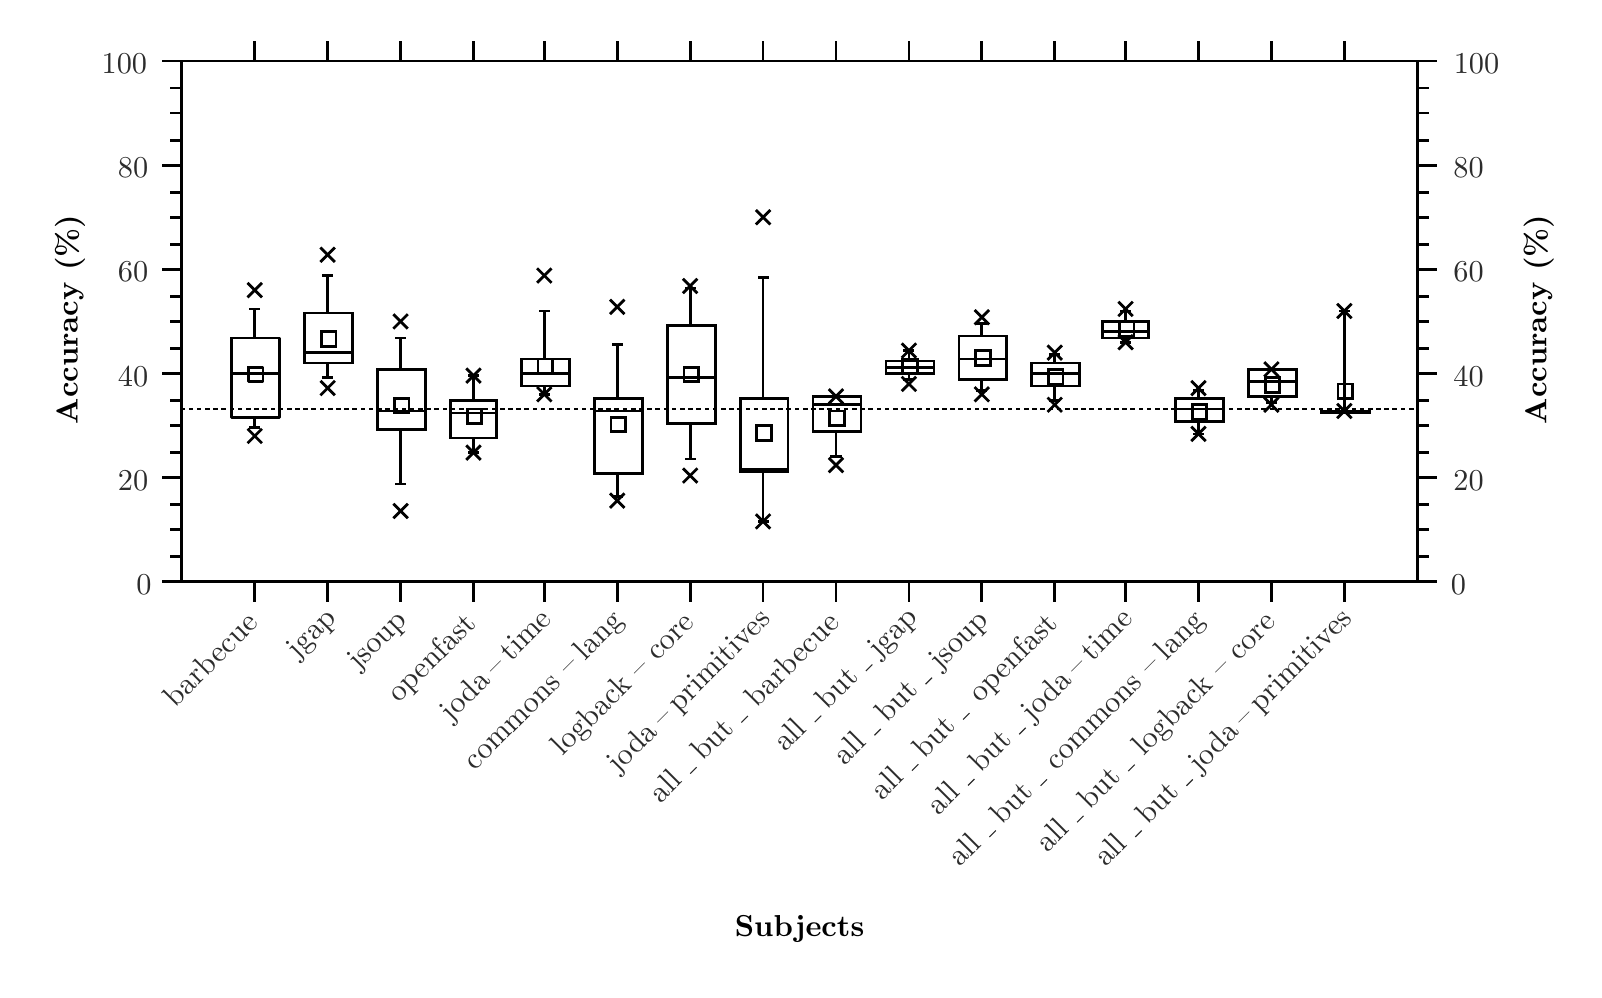
\begin{tikzpicture}{0pt}{0pt}{742pt}{452pt}
	\clip(0pt,452pt) -- (558.587pt,452pt) -- (558.587pt,111.729pt) -- (0pt,111.729pt) -- (0pt,452pt);
\begin{scope}
	\clip(55.7081pt,439.955pt) -- (502.126pt,439.955pt) -- (502.126pt,251.752pt) -- (55.7081pt,251.752pt) -- (55.7081pt,439.955pt);
	\color[rgb]{0,0,0}
	\draw[line width=1pt, line join=bevel, line cap=rect](73.7756pt,339.831pt) -- (91.0903pt,339.831pt) -- (91.0903pt,311.224pt) -- (73.7756pt,311.224pt) -- (73.7756pt,339.831pt);
	\color[rgb]{0,0,0}
	\draw[line width=1pt, line join=bevel, line cap=rect](80.5509pt,307.46pt) -- (83.5622pt,307.46pt);
	\draw[line width=1pt, line join=bevel, line cap=rect](80.5509pt,350.37pt) -- (83.5622pt,350.37pt);
	\draw[line width=1pt, line join=bevel, line cap=rect](82.0566pt,350.37pt) -- (82.0566pt,339.831pt);
	\draw[line width=1pt, line join=bevel, line cap=rect](82.0566pt,307.46pt) -- (82.0566pt,311.224pt);
	\draw[line width=1pt, line join=bevel, line cap=rect](73.7756pt,327.033pt) -- (90.3375pt,327.033pt);
	\draw[line width=1pt, line join=bevel, line cap=rect](79.7981pt,306.707pt) -- (84.315pt,302.19pt);
	\draw[line width=1pt, line join=bevel, line cap=rect](79.7981pt,302.19pt) -- (84.315pt,306.707pt);
	\draw[line width=1pt, line join=bevel, line cap=rect](79.7981pt,359.404pt) -- (84.315pt,354.887pt);
	\draw[line width=1pt, line join=bevel, line cap=rect](79.7981pt,354.887pt) -- (84.315pt,359.404pt);
	\draw[line width=1pt, line join=bevel, line cap=rect](79.7981pt,329.292pt) -- (85.0678pt,329.292pt) -- (85.0678pt,324.022pt) -- (79.7981pt,324.022pt) -- (79.7981pt,329.292pt);
	\draw[line width=1pt, line join=miter, line cap=rect](100.124pt,348.865pt) -- (117.439pt,348.865pt) -- (117.439pt,330.797pt) -- (100.124pt,330.797pt) -- (100.124pt,348.865pt);
	\draw[line width=1pt, line join=miter, line cap=rect](106.899pt,325.528pt) -- (109.911pt,325.528pt);
	\draw[line width=1pt, line join=miter, line cap=rect](106.899pt,362.415pt) -- (109.911pt,362.415pt);
	\draw[line width=1pt, line join=miter, line cap=rect](108.405pt,362.415pt) -- (108.405pt,348.865pt);
	\draw[line width=1pt, line join=miter, line cap=rect](108.405pt,325.528pt) -- (108.405pt,330.797pt);
	\draw[line width=1pt, line join=miter, line cap=rect](100.124pt,334.561pt) -- (116.686pt,334.561pt);
	\draw[line width=1pt, line join=miter, line cap=rect](106.147pt,324.022pt) -- (110.663pt,319.505pt);
	\draw[line width=1pt, line join=miter, line cap=rect](106.147pt,319.505pt) -- (110.663pt,324.022pt);
	\draw[line width=1pt, line join=miter, line cap=rect](106.147pt,372.202pt) -- (110.663pt,367.685pt);
	\draw[line width=1pt, line join=miter, line cap=rect](106.147pt,367.685pt) -- (110.663pt,372.202pt);
	\draw[line width=1pt, line join=miter, line cap=rect](106.147pt,342.089pt) -- (111.416pt,342.089pt) -- (111.416pt,336.82pt) -- (106.147pt,336.82pt) -- (106.147pt,342.089pt);
	\draw[line width=1pt, line join=miter, line cap=rect](126.472pt,328.539pt) -- (143.787pt,328.539pt) -- (143.787pt,306.707pt) -- (126.472pt,306.707pt) -- (126.472pt,328.539pt);
	\draw[line width=1pt, line join=miter, line cap=rect](133.248pt,287.134pt) -- (136.259pt,287.134pt);
	\draw[line width=1pt, line join=miter, line cap=rect](133.248pt,339.831pt) -- (136.259pt,339.831pt);
	\draw[line width=1pt, line join=miter, line cap=rect](134.753pt,339.831pt) -- (134.753pt,328.539pt);
	\draw[line width=1pt, line join=miter, line cap=rect](134.753pt,287.134pt) -- (134.753pt,306.707pt);
	\draw[line width=1pt, line join=miter, line cap=rect](126.472pt,313.482pt) -- (143.034pt,313.482pt);
	\draw[line width=1pt, line join=miter, line cap=rect](132.495pt,279.606pt) -- (137.012pt,275.089pt);
	\draw[line width=1pt, line join=miter, line cap=rect](132.495pt,275.089pt) -- (137.012pt,279.606pt);
	\draw[line width=1pt, line join=miter, line cap=rect](132.495pt,348.112pt) -- (137.012pt,343.595pt);
	\draw[line width=1pt, line join=miter, line cap=rect](132.495pt,343.595pt) -- (137.012pt,348.112pt);
	\draw[line width=1pt, line join=miter, line cap=rect](132.495pt,317.999pt) -- (137.765pt,317.999pt) -- (137.765pt,312.73pt) -- (132.495pt,312.73pt) -- (132.495pt,317.999pt);
	\draw[line width=1pt, line join=miter, line cap=rect](152.821pt,317.247pt) -- (169.383pt,317.247pt) -- (169.383pt,303.696pt) -- (152.821pt,303.696pt) -- (152.821pt,317.247pt);
	\draw[line width=1pt, line join=miter, line cap=rect](159.596pt,298.426pt) -- (162.607pt,298.426pt);
	\draw[line width=1pt, line join=miter, line cap=rect](159.596pt,326.28pt) -- (162.607pt,326.28pt);
	\draw[line width=1pt, line join=miter, line cap=rect](161.102pt,326.28pt) -- (161.102pt,317.247pt);
	\draw[line width=1pt, line join=miter, line cap=rect](161.102pt,298.426pt) -- (161.102pt,303.696pt);
	\draw[line width=1pt, line join=miter, line cap=rect](152.821pt,312.73pt) -- (169.383pt,312.73pt);
	\draw[line width=1pt, line join=miter, line cap=rect](158.843pt,300.685pt) -- (163.36pt,296.168pt);
	\draw[line width=1pt, line join=miter, line cap=rect](158.843pt,296.168pt) -- (163.36pt,300.685pt);
	\draw[line width=1pt, line join=miter, line cap=rect](158.843pt,328.539pt) -- (163.36pt,324.022pt);
	\draw[line width=1pt, line join=miter, line cap=rect](158.843pt,324.022pt) -- (163.36pt,328.539pt);
	\draw[line width=1pt, line join=miter, line cap=rect](158.843pt,314.235pt) -- (164.113pt,314.235pt) -- (164.113pt,308.966pt) -- (158.843pt,308.966pt) -- (158.843pt,314.235pt);
	\draw[line width=1pt, line join=miter, line cap=rect](178.417pt,332.303pt) -- (195.731pt,332.303pt) -- (195.731pt,322.516pt) -- (178.417pt,322.516pt) -- (178.417pt,332.303pt);
	\draw[line width=1pt, line join=miter, line cap=rect](185.192pt,319.505pt) -- (188.203pt,319.505pt);
	\draw[line width=1pt, line join=miter, line cap=rect](185.192pt,349.618pt) -- (188.203pt,349.618pt);
	\draw[line width=1pt, line join=miter, line cap=rect](186.697pt,349.618pt) -- (186.697pt,332.303pt);
	\draw[line width=1pt, line join=miter, line cap=rect](186.697pt,319.505pt) -- (186.697pt,322.516pt);
	\draw[line width=1pt, line join=miter, line cap=rect](178.417pt,327.033pt) -- (194.978pt,327.033pt);
	\draw[line width=1pt, line join=miter, line cap=rect](184.439pt,321.763pt) -- (188.956pt,317.247pt);
	\draw[line width=1pt, line join=miter, line cap=rect](184.439pt,317.247pt) -- (188.956pt,321.763pt);
	\draw[line width=1pt, line join=miter, line cap=rect](184.439pt,364.674pt) -- (188.956pt,360.157pt);
	\draw[line width=1pt, line join=miter, line cap=rect](184.439pt,360.157pt) -- (188.956pt,364.674pt);
	\draw[line width=1pt, line join=miter, line cap=rect](184.439pt,332.303pt) -- (189.709pt,332.303pt) -- (189.709pt,327.033pt) -- (184.439pt,327.033pt) -- (184.439pt,332.303pt);
	\draw[line width=1pt, line join=miter, line cap=rect](204.765pt,317.999pt) -- (222.08pt,317.999pt) -- (222.08pt,290.898pt) -- (204.765pt,290.898pt) -- (204.765pt,317.999pt);
	\draw[line width=1pt, line join=miter, line cap=rect](211.54pt,282.617pt) -- (214.552pt,282.617pt);
	\draw[line width=1pt, line join=miter, line cap=rect](211.54pt,337.572pt) -- (214.552pt,337.572pt);
	\draw[line width=1pt, line join=miter, line cap=rect](213.046pt,337.572pt) -- (213.046pt,317.999pt);
	\draw[line width=1pt, line join=miter, line cap=rect](213.046pt,282.617pt) -- (213.046pt,290.898pt);
	\draw[line width=1pt, line join=miter, line cap=rect](204.765pt,313.482pt) -- (221.327pt,313.482pt);
	\draw[line width=1pt, line join=miter, line cap=rect](210.787pt,283.37pt) -- (215.304pt,278.853pt);
	\draw[line width=1pt, line join=miter, line cap=rect](210.787pt,278.853pt) -- (215.304pt,283.37pt);
	\draw[line width=1pt, line join=miter, line cap=rect](210.787pt,353.382pt) -- (215.304pt,348.865pt);
	\draw[line width=1pt, line join=miter, line cap=rect](210.787pt,348.865pt) -- (215.304pt,353.382pt);
	\draw[line width=1pt, line join=miter, line cap=rect](210.787pt,311.224pt) -- (216.057pt,311.224pt) -- (216.057pt,305.954pt) -- (210.787pt,305.954pt) -- (210.787pt,311.224pt);
	\draw[line width=1pt, line join=miter, line cap=rect](231.113pt,344.348pt) -- (248.428pt,344.348pt) -- (248.428pt,308.966pt) -- (231.113pt,308.966pt) -- (231.113pt,344.348pt);
	\draw[line width=1pt, line join=miter, line cap=rect](237.889pt,296.168pt) -- (240.9pt,296.168pt);
	\draw[line width=1pt, line join=miter, line cap=rect](237.889pt,357.898pt) -- (240.9pt,357.898pt);
	\draw[line width=1pt, line join=miter, line cap=rect](239.394pt,357.898pt) -- (239.394pt,344.348pt);
	\draw[line width=1pt, line join=miter, line cap=rect](239.394pt,296.168pt) -- (239.394pt,308.966pt);
	\draw[line width=1pt, line join=miter, line cap=rect](231.113pt,325.528pt) -- (247.675pt,325.528pt);
	\draw[line width=1pt, line join=miter, line cap=rect](237.136pt,292.404pt) -- (241.653pt,287.887pt);
	\draw[line width=1pt, line join=miter, line cap=rect](237.136pt,287.887pt) -- (241.653pt,292.404pt);
	\draw[line width=1pt, line join=miter, line cap=rect](237.136pt,360.91pt) -- (241.653pt,356.393pt);
	\draw[line width=1pt, line join=miter, line cap=rect](237.136pt,356.393pt) -- (241.653pt,360.91pt);
	\draw[line width=1pt, line join=miter, line cap=rect](237.136pt,329.292pt) -- (242.406pt,329.292pt) -- (242.406pt,324.022pt) -- (237.136pt,324.022pt) -- (237.136pt,329.292pt);
	\draw[line width=1pt, line join=miter, line cap=rect](257.462pt,317.999pt) -- (274.777pt,317.999pt) -- (274.777pt,291.651pt) -- (257.462pt,291.651pt) -- (257.462pt,317.999pt);
	\draw[line width=1pt, line join=miter, line cap=rect](264.237pt,273.583pt) -- (267.248pt,273.583pt);
	\draw[line width=1pt, line join=miter, line cap=rect](264.237pt,361.663pt) -- (267.248pt,361.663pt);
	\draw[line width=1pt, line join=miter, line cap=rect](265.743pt,361.663pt) -- (265.743pt,317.999pt);
	\draw[line width=1pt, line join=miter, line cap=rect](265.743pt,273.583pt) -- (265.743pt,291.651pt);
	\draw[line width=1pt, line join=miter, line cap=rect](257.462pt,292.404pt) -- (274.024pt,292.404pt);
	\draw[line width=1pt, line join=miter, line cap=rect](263.484pt,275.842pt) -- (268.001pt,271.325pt);
	\draw[line width=1pt, line join=miter, line cap=rect](263.484pt,271.325pt) -- (268.001pt,275.842pt);
	\draw[line width=1pt, line join=miter, line cap=rect](263.484pt,385.752pt) -- (268.001pt,381.236pt);
	\draw[line width=1pt, line join=miter, line cap=rect](263.484pt,381.236pt) -- (268.001pt,385.752pt);
	\draw[line width=1pt, line join=miter, line cap=rect](263.484pt,308.213pt) -- (268.754pt,308.213pt) -- (268.754pt,302.943pt) -- (263.484pt,302.943pt) -- (263.484pt,308.213pt);
	\draw[line width=1pt, line join=miter, line cap=rect](283.81pt,318.752pt) -- (301.125pt,318.752pt) -- (301.125pt,305.954pt) -- (283.81pt,305.954pt) -- (283.81pt,318.752pt);
	\draw[line width=1pt, line join=miter, line cap=rect](290.586pt,296.921pt) -- (293.597pt,296.921pt);
	\draw[line width=1pt, line join=miter, line cap=rect](290.586pt,318.752pt) -- (293.597pt,318.752pt);
	\draw[line width=1pt, line join=miter, line cap=rect](292.091pt,296.921pt) -- (292.091pt,305.954pt);
	\draw[line width=1pt, line join=miter, line cap=rect](283.81pt,315.741pt) -- (300.372pt,315.741pt);
	\draw[line width=1pt, line join=miter, line cap=rect](289.833pt,296.168pt) -- (294.35pt,291.651pt);
	\draw[line width=1pt, line join=miter, line cap=rect](289.833pt,291.651pt) -- (294.35pt,296.168pt);
	\draw[line width=1pt, line join=miter, line cap=rect](289.833pt,321.011pt) -- (294.35pt,316.494pt);
	\draw[line width=1pt, line join=miter, line cap=rect](289.833pt,316.494pt) -- (294.35pt,321.011pt);
	\draw[line width=1pt, line join=miter, line cap=rect](289.833pt,313.482pt) -- (295.103pt,313.482pt) -- (295.103pt,308.213pt) -- (289.833pt,308.213pt) -- (289.833pt,313.482pt);
	\draw[line width=1pt, line join=miter, line cap=rect](310.159pt,331.55pt) -- (327.473pt,331.55pt) -- (327.473pt,327.033pt) -- (310.159pt,327.033pt) -- (310.159pt,331.55pt);
	\draw[line width=1pt, line join=miter, line cap=rect](316.934pt,324.775pt) -- (319.945pt,324.775pt);
	\draw[line width=1pt, line join=miter, line cap=rect](316.934pt,335.314pt) -- (319.945pt,335.314pt);
	\draw[line width=1pt, line join=miter, line cap=rect](318.44pt,335.314pt) -- (318.44pt,331.55pt);
	\draw[line width=1pt, line join=miter, line cap=rect](318.44pt,324.775pt) -- (318.44pt,327.033pt);
	\draw[line width=1pt, line join=miter, line cap=rect](310.159pt,329.292pt) -- (326.721pt,329.292pt);
	\draw[line width=1pt, line join=miter, line cap=rect](316.181pt,325.528pt) -- (320.698pt,321.011pt);
	\draw[line width=1pt, line join=miter, line cap=rect](316.181pt,321.011pt) -- (320.698pt,325.528pt);
	\draw[line width=1pt, line join=miter, line cap=rect](316.181pt,337.572pt) -- (320.698pt,333.056pt);
	\draw[line width=1pt, line join=miter, line cap=rect](316.181pt,333.056pt) -- (320.698pt,337.572pt);
	\draw[line width=1pt, line join=miter, line cap=rect](316.181pt,332.303pt) -- (321.451pt,332.303pt) -- (321.451pt,327.033pt) -- (316.181pt,327.033pt) -- (316.181pt,332.303pt);
	\draw[line width=1pt, line join=miter, line cap=rect](336.507pt,340.584pt) -- (353.822pt,340.584pt) -- (353.822pt,324.775pt) -- (336.507pt,324.775pt) -- (336.507pt,340.584pt);
	\draw[line width=1pt, line join=miter, line cap=rect](343.282pt,321.011pt) -- (346.294pt,321.011pt);
	\draw[line width=1pt, line join=miter, line cap=rect](343.282pt,345.101pt) -- (346.294pt,345.101pt);
	\draw[line width=1pt, line join=miter, line cap=rect](344.788pt,345.101pt) -- (344.788pt,340.584pt);
	\draw[line width=1pt, line join=miter, line cap=rect](344.788pt,321.011pt) -- (344.788pt,324.775pt);
	\draw[line width=1pt, line join=miter, line cap=rect](336.507pt,332.303pt) -- (353.069pt,332.303pt);
	\draw[line width=1pt, line join=miter, line cap=rect](342.53pt,321.763pt) -- (347.047pt,317.247pt);
	\draw[line width=1pt, line join=miter, line cap=rect](342.53pt,317.247pt) -- (347.047pt,321.763pt);
	\draw[line width=1pt, line join=miter, line cap=rect](342.53pt,349.618pt) -- (347.047pt,345.101pt);
	\draw[line width=1pt, line join=miter, line cap=rect](342.53pt,345.101pt) -- (347.047pt,349.618pt);
	\draw[line width=1pt, line join=miter, line cap=rect](342.53pt,335.314pt) -- (347.799pt,335.314pt) -- (347.799pt,330.044pt) -- (342.53pt,330.044pt) -- (342.53pt,335.314pt);
	\draw[line width=1pt, line join=miter, line cap=rect](362.856pt,330.797pt) -- (380.17pt,330.797pt) -- (380.17pt,322.516pt) -- (362.856pt,322.516pt) -- (362.856pt,330.797pt);
	\draw[line width=1pt, line join=miter, line cap=rect](369.631pt,317.247pt) -- (372.642pt,317.247pt);
	\draw[line width=1pt, line join=miter, line cap=rect](369.631pt,333.808pt) -- (372.642pt,333.808pt);
	\draw[line width=1pt, line join=miter, line cap=rect](371.137pt,333.808pt) -- (371.137pt,330.797pt);
	\draw[line width=1pt, line join=miter, line cap=rect](371.137pt,317.247pt) -- (371.137pt,322.516pt);
	\draw[line width=1pt, line join=miter, line cap=rect](362.856pt,327.033pt) -- (379.418pt,327.033pt);
	\draw[line width=1pt, line join=miter, line cap=rect](368.878pt,317.999pt) -- (373.395pt,313.482pt);
	\draw[line width=1pt, line join=miter, line cap=rect](368.878pt,313.482pt) -- (373.395pt,317.999pt);
	\draw[line width=1pt, line join=miter, line cap=rect](368.878pt,336.82pt) -- (373.395pt,332.303pt);
	\draw[line width=1pt, line join=miter, line cap=rect](368.878pt,332.303pt) -- (373.395pt,336.82pt);
	\draw[line width=1pt, line join=miter, line cap=rect](368.878pt,328.539pt) -- (374.148pt,328.539pt) -- (374.148pt,323.269pt) -- (368.878pt,323.269pt) -- (368.878pt,328.539pt);
	\draw[line width=1pt, line join=miter, line cap=rect](388.451pt,345.853pt) -- (405.013pt,345.853pt) -- (405.013pt,339.831pt) -- (388.451pt,339.831pt) -- (388.451pt,345.853pt);
	\draw[line width=1pt, line join=miter, line cap=rect](395.227pt,338.325pt) -- (398.238pt,338.325pt);
	\draw[line width=1pt, line join=miter, line cap=rect](395.227pt,349.618pt) -- (398.238pt,349.618pt);
	\draw[line width=1pt, line join=miter, line cap=rect](396.732pt,349.618pt) -- (396.732pt,345.853pt);
	\draw[line width=1pt, line join=miter, line cap=rect](396.732pt,338.325pt) -- (396.732pt,339.831pt);
	\draw[line width=1pt, line join=miter, line cap=rect](388.451pt,342.089pt) -- (405.013pt,342.089pt);
	\draw[line width=1pt, line join=miter, line cap=rect](394.474pt,340.584pt) -- (398.991pt,336.067pt);
	\draw[line width=1pt, line join=miter, line cap=rect](394.474pt,336.067pt) -- (398.991pt,340.584pt);
	\draw[line width=1pt, line join=miter, line cap=rect](394.474pt,352.629pt) -- (398.991pt,348.112pt);
	\draw[line width=1pt, line join=miter, line cap=rect](394.474pt,348.112pt) -- (398.991pt,352.629pt);
	\draw[line width=1pt, line join=miter, line cap=rect](394.474pt,345.853pt) -- (399.743pt,345.853pt) -- (399.743pt,340.584pt) -- (394.474pt,340.584pt) -- (394.474pt,345.853pt);
	\draw[line width=1pt, line join=miter, line cap=rect](414.8pt,317.999pt) -- (432.114pt,317.999pt) -- (432.114pt,309.718pt) -- (414.8pt,309.718pt) -- (414.8pt,317.999pt);
	\draw[line width=1pt, line join=miter, line cap=rect](421.575pt,305.202pt) -- (424.586pt,305.202pt);
	\draw[line width=1pt, line join=miter, line cap=rect](421.575pt,321.011pt) -- (424.586pt,321.011pt);
	\draw[line width=1pt, line join=miter, line cap=rect](423.081pt,321.011pt) -- (423.081pt,317.999pt);
	\draw[line width=1pt, line join=miter, line cap=rect](423.081pt,305.202pt) -- (423.081pt,309.718pt);
	\draw[line width=1pt, line join=miter, line cap=rect](414.8pt,314.235pt) -- (431.362pt,314.235pt);
	\draw[line width=1pt, line join=miter, line cap=rect](420.822pt,307.46pt) -- (425.339pt,302.943pt);
	\draw[line width=1pt, line join=miter, line cap=rect](420.822pt,302.943pt) -- (425.339pt,307.46pt);
	\draw[line width=1pt, line join=miter, line cap=rect](420.822pt,324.022pt) -- (425.339pt,319.505pt);
	\draw[line width=1pt, line join=miter, line cap=rect](420.822pt,319.505pt) -- (425.339pt,324.022pt);
	\draw[line width=1pt, line join=miter, line cap=rect](420.822pt,315.741pt) -- (426.092pt,315.741pt) -- (426.092pt,310.471pt) -- (420.822pt,310.471pt) -- (420.822pt,315.741pt);
	\draw[line width=1pt, line join=miter, line cap=rect](441.148pt,328.539pt) -- (458.463pt,328.539pt) -- (458.463pt,318.752pt) -- (441.148pt,318.752pt) -- (441.148pt,328.539pt);
	\draw[line width=1pt, line join=miter, line cap=rect](447.923pt,316.494pt) -- (450.935pt,316.494pt);
	\draw[line width=1pt, line join=miter, line cap=rect](447.923pt,328.539pt) -- (450.935pt,328.539pt);
	\draw[line width=1pt, line join=miter, line cap=rect](449.429pt,316.494pt) -- (449.429pt,318.752pt);
	\draw[line width=1pt, line join=miter, line cap=rect](441.148pt,324.022pt) -- (457.71pt,324.022pt);
	\draw[line width=1pt, line join=miter, line cap=rect](447.171pt,317.999pt) -- (451.688pt,313.482pt);
	\draw[line width=1pt, line join=miter, line cap=rect](447.171pt,313.482pt) -- (451.688pt,317.999pt);
	\draw[line width=1pt, line join=miter, line cap=rect](447.171pt,330.797pt) -- (451.688pt,326.28pt);
	\draw[line width=1pt, line join=miter, line cap=rect](447.171pt,326.28pt) -- (451.688pt,330.797pt);
	\draw[line width=1pt, line join=miter, line cap=rect](447.171pt,325.528pt) -- (452.44pt,325.528pt) -- (452.44pt,320.258pt) -- (447.171pt,320.258pt) -- (447.171pt,325.528pt);
	\draw[line width=1pt, line join=miter, line cap=rect](467.497pt,313.482pt) -- (484.811pt,313.482pt) -- (484.811pt,312.73pt) -- (467.497pt,312.73pt) -- (467.497pt,313.482pt);
	\draw[line width=1pt, line join=miter, line cap=rect](474.272pt,313.482pt) -- (477.283pt,313.482pt);
	\draw[line width=1pt, line join=miter, line cap=rect](474.272pt,349.618pt) -- (477.283pt,349.618pt);
	\draw[line width=1pt, line join=miter, line cap=rect](475.777pt,349.618pt) -- (475.777pt,313.482pt);
	\draw[line width=1pt, line join=miter, line cap=rect](467.497pt,313.482pt) -- (484.058pt,313.482pt);
	\draw[line width=1pt, line join=miter, line cap=rect](473.519pt,315.741pt) -- (478.036pt,311.224pt);
	\draw[line width=1pt, line join=miter, line cap=rect](473.519pt,311.224pt) -- (478.036pt,315.741pt);
	\draw[line width=1pt, line join=miter, line cap=rect](473.519pt,351.876pt) -- (478.036pt,347.359pt);
	\draw[line width=1pt, line join=miter, line cap=rect](473.519pt,347.359pt) -- (478.036pt,351.876pt);
	\draw[line width=1pt, line join=miter, line cap=rect](473.519pt,323.269pt) -- (478.789pt,323.269pt) -- (478.789pt,317.999pt) -- (473.519pt,317.999pt) -- (473.519pt,323.269pt);
	\draw[line width=1pt, dash pattern=on 0.024cm off 0.08cm, dash phase=0pt, line join=miter, line cap=rect](55.7081pt,314.235pt) -- (528.474pt,314.235pt);
\end{scope}
\begin{scope}
	\color[rgb]{0,0,0}
	\pgftext[center, base, at={\pgfpoint{18.0675pt}{346.606pt}},rotate=90]{\fontsize{11}{0}\selectfont{\textbf{Accuracy (\%)}}}
	\color[rgb]{0.172549,0.172549,0.172549}
	\pgftext[center, base, at={\pgfpoint{42.0163pt}{247.235pt}}]{\fontsize{11}{0}\selectfont{0}}
	\pgftext[center, base, at={\pgfpoint{38.1111pt}{284.876pt}}]{\fontsize{11}{0}\selectfont{20}}
	\pgftext[center, base, at={\pgfpoint{38.1111pt}{322.516pt}}]{\fontsize{11}{0}\selectfont{40}}
	\pgftext[center, base, at={\pgfpoint{38.1111pt}{360.157pt}}]{\fontsize{11}{0}\selectfont{60}}
	\pgftext[center, base, at={\pgfpoint{38.1111pt}{397.798pt}}]{\fontsize{11}{0}\selectfont{80}}
	\pgftext[center, base, at={\pgfpoint{34.9587pt}{435.438pt}}]{\fontsize{11}{0}\selectfont{100}}
	\color[rgb]{0,0,0}
	\draw[line width=1pt, line join=bevel, line cap=rect](55.7081pt,260.786pt) -- (51.9441pt,260.786pt);
	\draw[line width=1pt, line join=bevel, line cap=rect](55.7081pt,279.606pt) -- (51.9441pt,279.606pt);
	\draw[line width=1pt, line join=bevel, line cap=rect](55.7081pt,298.426pt) -- (51.9441pt,298.426pt);
	\draw[line width=1pt, line join=bevel, line cap=rect](55.7081pt,317.247pt) -- (51.9441pt,317.247pt);
	\draw[line width=1pt, line join=bevel, line cap=rect](55.7081pt,336.067pt) -- (51.9441pt,336.067pt);
	\draw[line width=1pt, line join=bevel, line cap=rect](55.7081pt,354.887pt) -- (51.9441pt,354.887pt);
	\draw[line width=1pt, line join=bevel, line cap=rect](55.7081pt,373.707pt) -- (51.9441pt,373.707pt);
	\draw[line width=1pt, line join=bevel, line cap=rect](55.7081pt,392.528pt) -- (51.9441pt,392.528pt);
	\draw[line width=1pt, line join=bevel, line cap=rect](55.7081pt,411.348pt) -- (51.9441pt,411.348pt);
	\draw[line width=1pt, line join=bevel, line cap=rect](55.7081pt,430.168pt) -- (51.9441pt,430.168pt);
	\draw[line width=1pt, line join=bevel, line cap=rect](55.7081pt,270.572pt) -- (51.9441pt,270.572pt);
	\draw[line width=1pt, line join=bevel, line cap=rect](55.7081pt,308.213pt) -- (51.9441pt,308.213pt);
	\draw[line width=1pt, line join=bevel, line cap=rect](55.7081pt,345.853pt) -- (51.9441pt,345.853pt);
	\draw[line width=1pt, line join=bevel, line cap=rect](55.7081pt,383.494pt) -- (51.9441pt,383.494pt);
	\draw[line width=1pt, line join=bevel, line cap=rect](55.7081pt,421.135pt) -- (51.9441pt,421.135pt);
	\draw[line width=1pt, line join=bevel, line cap=rect](55.7081pt,251.752pt) -- (48.9328pt,251.752pt);
	\draw[line width=1pt, line join=bevel, line cap=rect](55.7081pt,289.393pt) -- (48.9328pt,289.393pt);
	\draw[line width=1pt, line join=bevel, line cap=rect](55.7081pt,327.033pt) -- (48.9328pt,327.033pt);
	\draw[line width=1pt, line join=bevel, line cap=rect](55.7081pt,364.674pt) -- (48.9328pt,364.674pt);
	\draw[line width=1pt, line join=bevel, line cap=rect](55.7081pt,402.314pt) -- (48.9328pt,402.314pt);
	\draw[line width=1pt, line join=bevel, line cap=rect](55.7081pt,439.955pt) -- (48.9328pt,439.955pt);
	\draw[line width=1pt, line join=bevel, line cap=rect](55.7081pt,439.955pt) -- (55.7081pt,251.752pt);
	\pgftext[center, base, at={\pgfpoint{548.8pt}{346.606pt}},rotate=90]{\fontsize{11}{0}\selectfont{\textbf{Accuracy (\%)}}}
	\color[rgb]{0.172549,0.172549,0.172549}
	\pgftext[center, base, at={\pgfpoint{517.041pt}{247.235pt}}]{\fontsize{11}{0}\selectfont{0}}
	\pgftext[center, base, at={\pgfpoint{520.664pt}{284.876pt}}]{\fontsize{11}{0}\selectfont{20}}
	\pgftext[center, base, at={\pgfpoint{520.664pt}{322.516pt}}]{\fontsize{11}{0}\selectfont{40}}
	\pgftext[center, base, at={\pgfpoint{520.664pt}{360.157pt}}]{\fontsize{11}{0}\selectfont{60}}
	\pgftext[center, base, at={\pgfpoint{520.664pt}{397.798pt}}]{\fontsize{11}{0}\selectfont{80}}
	\pgftext[center, base, at={\pgfpoint{523.534pt}{435.438pt}}]{\fontsize{11}{0}\selectfont{100}}
	\color[rgb]{0,0,0}
	\draw[line width=1pt, line join=bevel, line cap=rect](502.126pt,260.786pt) -- (505.89pt,260.786pt);
	\draw[line width=1pt, line join=bevel, line cap=rect](502.126pt,279.606pt) -- (505.89pt,279.606pt);
	\draw[line width=1pt, line join=bevel, line cap=rect](502.126pt,298.426pt) -- (505.89pt,298.426pt);
	\draw[line width=1pt, line join=bevel, line cap=rect](502.126pt,317.247pt) -- (505.89pt,317.247pt);
	\draw[line width=1pt, line join=bevel, line cap=rect](502.126pt,336.067pt) -- (505.89pt,336.067pt);
	\draw[line width=1pt, line join=bevel, line cap=rect](502.126pt,354.887pt) -- (505.89pt,354.887pt);
	\draw[line width=1pt, line join=bevel, line cap=rect](502.126pt,373.707pt) -- (505.89pt,373.707pt);
	\draw[line width=1pt, line join=bevel, line cap=rect](502.126pt,392.528pt) -- (505.89pt,392.528pt);
	\draw[line width=1pt, line join=bevel, line cap=rect](502.126pt,411.348pt) -- (505.89pt,411.348pt);
	\draw[line width=1pt, line join=bevel, line cap=rect](502.126pt,430.168pt) -- (505.89pt,430.168pt);
	\draw[line width=1pt, line join=bevel, line cap=rect](502.126pt,270.572pt) -- (505.89pt,270.572pt);
	\draw[line width=1pt, line join=bevel, line cap=rect](502.126pt,308.213pt) -- (505.89pt,308.213pt);
	\draw[line width=1pt, line join=bevel, line cap=rect](502.126pt,345.853pt) -- (505.89pt,345.853pt);
	\draw[line width=1pt, line join=bevel, line cap=rect](502.126pt,383.494pt) -- (505.89pt,383.494pt);
	\draw[line width=1pt, line join=bevel, line cap=rect](502.126pt,421.135pt) -- (505.89pt,421.135pt);
	\draw[line width=1pt, line join=bevel, line cap=rect](502.126pt,251.752pt) -- (508.901pt,251.752pt);
	\draw[line width=1pt, line join=bevel, line cap=rect](502.126pt,289.393pt) -- (508.901pt,289.393pt);
	\draw[line width=1pt, line join=bevel, line cap=rect](502.126pt,327.033pt) -- (508.901pt,327.033pt);
	\draw[line width=1pt, line join=bevel, line cap=rect](502.126pt,364.674pt) -- (508.901pt,364.674pt);
	\draw[line width=1pt, line join=bevel, line cap=rect](502.126pt,402.314pt) -- (508.901pt,402.314pt);
	\draw[line width=1pt, line join=bevel, line cap=rect](502.126pt,439.955pt) -- (508.901pt,439.955pt);
	\draw[line width=1pt, line join=bevel, line cap=rect](502.126pt,439.955pt) -- (502.126pt,251.752pt);
	\pgftext[center, base, at={\pgfpoint{278.917pt}{123.774pt}}]{\fontsize{11}{0}\selectfont{\textbf{Subjects}}}
	\color[rgb]{0.172549,0.172549,0.172549}
	\pgftext[center, base, at={\pgfpoint{68.4991pt}{221.267pt}},rotate=45]{\fontsize{11}{0}\selectfont{barbecue}}
	\pgftext[center, base, at={\pgfpoint{104.654pt}{231.073pt}},rotate=45]{\fontsize{11}{0}\selectfont{jgap}}
	\pgftext[center, base, at={\pgfpoint{128.445pt}{228.516pt}},rotate=45]{\fontsize{11}{0}\selectfont{jsoup}}
	\pgftext[center, base, at={\pgfpoint{148.222pt}{221.945pt}},rotate=45]{\fontsize{11}{0}\selectfont{openfast}}
	\pgftext[center, base, at={\pgfpoint{160.198pt}{208.325pt}},rotate=45]{\fontsize{11}{0}\selectfont{joda}}
	\pgftext[center, base, at={\pgfpoint{171.111pt}{219.238pt}},rotate=45]{\fontsize{11}{0}\selectfont{--}}
	\pgftext[center, base, at={\pgfpoint{182.11pt}{230.238pt}},rotate=45]{\fontsize{11}{0}\selectfont{time}}
	\pgftext[center, base, at={\pgfpoint{177.272pt}{199.051pt}},rotate=45]{\fontsize{11}{0}\selectfont{commons}}
	\pgftext[center, base, at={\pgfpoint{197.542pt}{219.321pt}},rotate=45]{\fontsize{11}{0}\selectfont{--}}
	\pgftext[center, base, at={\pgfpoint{208.405pt}{230.184pt}},rotate=45]{\fontsize{11}{0}\selectfont{lang}}
	\pgftext[center, base, at={\pgfpoint{205.896pt}{201.326pt}},rotate=45]{\fontsize{11}{0}\selectfont{logback}}
	\pgftext[center, base, at={\pgfpoint{223.117pt}{218.547pt}},rotate=45]{\fontsize{11}{0}\selectfont{--}}
	\pgftext[center, base, at={\pgfpoint{234.342pt}{229.772pt}},rotate=45]{\fontsize{11}{0}\selectfont{core}}
	\pgftext[center, base, at={\pgfpoint{220.612pt}{189.694pt}},rotate=45]{\fontsize{11}{0}\selectfont{joda}}
	\pgftext[center, base, at={\pgfpoint{231.525pt}{200.607pt}},rotate=45]{\fontsize{11}{0}\selectfont{--}}
	\pgftext[center, base, at={\pgfpoint{252.027pt}{221.109pt}},rotate=45]{\fontsize{11}{0}\selectfont{primitives}}
	\pgftext[center, base, at={\pgfpoint{232.684pt}{175.417pt}},rotate=45]{\fontsize{11}{0}\selectfont{all}}
	\pgftext[center, base, at={\pgfpoint{240.498pt}{183.231pt}},rotate=45]{\fontsize{11}{0}\selectfont{\_}}
	\pgftext[center, base, at={\pgfpoint{249.743pt}{192.476pt}},rotate=45]{\fontsize{11}{0}\selectfont{but}}
	\pgftext[center, base, at={\pgfpoint{258.988pt}{201.721pt}},rotate=45]{\fontsize{11}{0}\selectfont{\_}}
	\pgftext[center, base, at={\pgfpoint{278.584pt}{221.317pt}},rotate=45]{\fontsize{11}{0}\selectfont{barbecue}}
	\pgftext[center, base, at={\pgfpoint{277.663pt}{194.048pt}},rotate=45]{\fontsize{11}{0}\selectfont{all}}
	\pgftext[center, base, at={\pgfpoint{285.478pt}{201.862pt}},rotate=45]{\fontsize{11}{0}\selectfont{\_}}
	\pgftext[center, base, at={\pgfpoint{294.722pt}{211.107pt}},rotate=45]{\fontsize{11}{0}\selectfont{but}}
	\pgftext[center, base, at={\pgfpoint{303.967pt}{220.352pt}},rotate=45]{\fontsize{11}{0}\selectfont{\_}}
	\pgftext[center, base, at={\pgfpoint{314.738pt}{231.123pt}},rotate=45]{\fontsize{11}{0}\selectfont{jgap}}
	\pgftext[center, base, at={\pgfpoint{299.221pt}{189.257pt}},rotate=45]{\fontsize{11}{0}\selectfont{all}}
	\pgftext[center, base, at={\pgfpoint{307.035pt}{197.072pt}},rotate=45]{\fontsize{11}{0}\selectfont{\_}}
	\pgftext[center, base, at={\pgfpoint{316.28pt}{206.317pt}},rotate=45]{\fontsize{11}{0}\selectfont{but}}
	\pgftext[center, base, at={\pgfpoint{325.525pt}{215.561pt}},rotate=45]{\fontsize{11}{0}\selectfont{\_}}
	\pgftext[center, base, at={\pgfpoint{338.529pt}{228.566pt}},rotate=45]{\fontsize{11}{0}\selectfont{jsoup}}
	\pgftext[center, base, at={\pgfpoint{312.794pt}{176.482pt}},rotate=45]{\fontsize{11}{0}\selectfont{all}}
	\pgftext[center, base, at={\pgfpoint{320.608pt}{184.296pt}},rotate=45]{\fontsize{11}{0}\selectfont{\_}}
	\pgftext[center, base, at={\pgfpoint{329.853pt}{193.541pt}},rotate=45]{\fontsize{11}{0}\selectfont{but}}
	\pgftext[center, base, at={\pgfpoint{339.098pt}{202.786pt}},rotate=45]{\fontsize{11}{0}\selectfont{\_}}
	\pgftext[center, base, at={\pgfpoint{358.307pt}{221.995pt}},rotate=45]{\fontsize{11}{0}\selectfont{openfast}}
	\pgftext[center, base, at={\pgfpoint{333.066pt}{171.159pt}},rotate=45]{\fontsize{11}{0}\selectfont{all}}
	\pgftext[center, base, at={\pgfpoint{340.88pt}{178.973pt}},rotate=45]{\fontsize{11}{0}\selectfont{\_}}
	\pgftext[center, base, at={\pgfpoint{350.125pt}{188.218pt}},rotate=45]{\fontsize{11}{0}\selectfont{but}}
	\pgftext[center, base, at={\pgfpoint{359.37pt}{197.463pt}},rotate=45]{\fontsize{11}{0}\selectfont{\_}}
	\pgftext[center, base, at={\pgfpoint{370.283pt}{208.375pt}},rotate=45]{\fontsize{11}{0}\selectfont{joda}}
	\pgftext[center, base, at={\pgfpoint{381.195pt}{219.288pt}},rotate=45]{\fontsize{11}{0}\selectfont{--}}
	\pgftext[center, base, at={\pgfpoint{392.195pt}{230.287pt}},rotate=45]{\fontsize{11}{0}\selectfont{time}}
	\pgftext[center, base, at={\pgfpoint{340.783pt}{152.527pt}},rotate=45]{\fontsize{11}{0}\selectfont{all}}
	\pgftext[center, base, at={\pgfpoint{348.598pt}{160.342pt}},rotate=45]{\fontsize{11}{0}\selectfont{\_}}
	\pgftext[center, base, at={\pgfpoint{357.842pt}{169.587pt}},rotate=45]{\fontsize{11}{0}\selectfont{but}}
	\pgftext[center, base, at={\pgfpoint{367.087pt}{178.831pt}},rotate=45]{\fontsize{11}{0}\selectfont{\_}}
	\pgftext[center, base, at={\pgfpoint{387.357pt}{199.101pt}},rotate=45]{\fontsize{11}{0}\selectfont{commons}}
	\pgftext[center, base, at={\pgfpoint{407.627pt}{219.371pt}},rotate=45]{\fontsize{11}{0}\selectfont{--}}
	\pgftext[center, base, at={\pgfpoint{418.489pt}{230.233pt}},rotate=45]{\fontsize{11}{0}\selectfont{lang}}
	\pgftext[center, base, at={\pgfpoint{372.455pt}{157.851pt}},rotate=45]{\fontsize{11}{0}\selectfont{all}}
	\pgftext[center, base, at={\pgfpoint{380.269pt}{165.665pt}},rotate=45]{\fontsize{11}{0}\selectfont{\_}}
	\pgftext[center, base, at={\pgfpoint{389.514pt}{174.91pt}},rotate=45]{\fontsize{11}{0}\selectfont{but}}
	\pgftext[center, base, at={\pgfpoint{398.759pt}{184.155pt}},rotate=45]{\fontsize{11}{0}\selectfont{\_}}
	\pgftext[center, base, at={\pgfpoint{415.98pt}{201.376pt}},rotate=45]{\fontsize{11}{0}\selectfont{logback}}
	\pgftext[center, base, at={\pgfpoint{433.202pt}{218.597pt}},rotate=45]{\fontsize{11}{0}\selectfont{--}}
	\pgftext[center, base, at={\pgfpoint{444.426pt}{229.822pt}},rotate=45]{\fontsize{11}{0}\selectfont{core}}
	\pgftext[center, base, at={\pgfpoint{393.48pt}{152.527pt}},rotate=45]{\fontsize{11}{0}\selectfont{all}}
	\pgftext[center, base, at={\pgfpoint{401.294pt}{160.342pt}},rotate=45]{\fontsize{11}{0}\selectfont{\_}}
	\pgftext[center, base, at={\pgfpoint{410.539pt}{169.587pt}},rotate=45]{\fontsize{11}{0}\selectfont{but}}
	\pgftext[center, base, at={\pgfpoint{419.784pt}{178.831pt}},rotate=45]{\fontsize{11}{0}\selectfont{\_}}
	\pgftext[center, base, at={\pgfpoint{430.697pt}{189.744pt}},rotate=45]{\fontsize{11}{0}\selectfont{joda}}
	\pgftext[center, base, at={\pgfpoint{441.609pt}{200.656pt}},rotate=45]{\fontsize{11}{0}\selectfont{--}}
	\pgftext[center, base, at={\pgfpoint{462.112pt}{221.159pt}},rotate=45]{\fontsize{11}{0}\selectfont{primitives}}
	\color[rgb]{0,0,0}
	\draw[line width=1pt, line join=bevel, line cap=rect](82.0566pt,251.752pt) -- (82.0566pt,244.977pt);
	\draw[line width=1pt, line join=bevel, line cap=rect](108.405pt,251.752pt) -- (108.405pt,244.977pt);
	\draw[line width=1pt, line join=bevel, line cap=rect](134.753pt,251.752pt) -- (134.753pt,244.977pt);
	\draw[line width=1pt, line join=bevel, line cap=rect](161.102pt,251.752pt) -- (161.102pt,244.977pt);
	\draw[line width=1pt, line join=bevel, line cap=rect](186.697pt,251.752pt) -- (186.697pt,244.977pt);
	\draw[line width=1pt, line join=bevel, line cap=rect](213.046pt,251.752pt) -- (213.046pt,244.977pt);
	\draw[line width=1pt, line join=bevel, line cap=rect](239.394pt,251.752pt) -- (239.394pt,244.977pt);
	\draw[line width=1pt, line join=bevel, line cap=rect](265.743pt,251.752pt) -- (265.743pt,244.977pt);
	\draw[line width=1pt, line join=bevel, line cap=rect](292.091pt,251.752pt) -- (292.091pt,244.977pt);
	\draw[line width=1pt, line join=bevel, line cap=rect](318.44pt,251.752pt) -- (318.44pt,244.977pt);
	\draw[line width=1pt, line join=bevel, line cap=rect](344.788pt,251.752pt) -- (344.788pt,244.977pt);
	\draw[line width=1pt, line join=bevel, line cap=rect](371.137pt,251.752pt) -- (371.137pt,244.977pt);
	\draw[line width=1pt, line join=bevel, line cap=rect](396.732pt,251.752pt) -- (396.732pt,244.977pt);
	\draw[line width=1pt, line join=bevel, line cap=rect](423.081pt,251.752pt) -- (423.081pt,244.977pt);
	\draw[line width=1pt, line join=bevel, line cap=rect](449.429pt,251.752pt) -- (449.429pt,244.977pt);
	\draw[line width=1pt, line join=bevel, line cap=rect](475.777pt,251.752pt) -- (475.777pt,244.977pt);
	\draw[line width=1pt, line join=bevel, line cap=rect](55.7081pt,251.752pt) -- (502.126pt,251.752pt);
	\draw[line width=1pt, line join=bevel, line cap=rect](82.0566pt,439.955pt) -- (82.0566pt,446.73pt);
	\draw[line width=1pt, line join=bevel, line cap=rect](108.405pt,439.955pt) -- (108.405pt,446.73pt);
	\draw[line width=1pt, line join=bevel, line cap=rect](134.753pt,439.955pt) -- (134.753pt,446.73pt);
	\draw[line width=1pt, line join=bevel, line cap=rect](161.102pt,439.955pt) -- (161.102pt,446.73pt);
	\draw[line width=1pt, line join=bevel, line cap=rect](186.697pt,439.955pt) -- (186.697pt,446.73pt);
	\draw[line width=1pt, line join=bevel, line cap=rect](213.046pt,439.955pt) -- (213.046pt,446.73pt);
	\draw[line width=1pt, line join=bevel, line cap=rect](239.394pt,439.955pt) -- (239.394pt,446.73pt);
	\draw[line width=1pt, line join=bevel, line cap=rect](265.743pt,439.955pt) -- (265.743pt,446.73pt);
	\draw[line width=1pt, line join=bevel, line cap=rect](292.091pt,439.955pt) -- (292.091pt,446.73pt);
	\draw[line width=1pt, line join=bevel, line cap=rect](318.44pt,439.955pt) -- (318.44pt,446.73pt);
	\draw[line width=1pt, line join=bevel, line cap=rect](344.788pt,439.955pt) -- (344.788pt,446.73pt);
	\draw[line width=1pt, line join=bevel, line cap=rect](371.137pt,439.955pt) -- (371.137pt,446.73pt);
	\draw[line width=1pt, line join=bevel, line cap=rect](396.732pt,439.955pt) -- (396.732pt,446.73pt);
	\draw[line width=1pt, line join=bevel, line cap=rect](423.081pt,439.955pt) -- (423.081pt,446.73pt);
	\draw[line width=1pt, line join=bevel, line cap=rect](449.429pt,439.955pt) -- (449.429pt,446.73pt);
	\draw[line width=1pt, line join=bevel, line cap=rect](475.777pt,439.955pt) -- (475.777pt,446.73pt);
	\draw[line width=1pt, line join=bevel, line cap=rect](55.7081pt,439.955pt) -- (502.126pt,439.955pt);
\end{scope}
\end{tikzpicture}

  \end{adjustbox}
  \caption{Class-level training and prediction accuracy over the 8 subjects and sets of \emph{all\_but\_<subject>} using generalized parameters [\emph{cost}=100, \emph{gamma}=0.01].}
  \vspace{2mm}
  \hrule
  \label{fig:prediction_with_parameters_class_graph}
\end{figure}

\begin{figure}[ht!]
  \centering
  \begin{adjustbox}{max size={.95\textwidth}{.95\textheight}}
    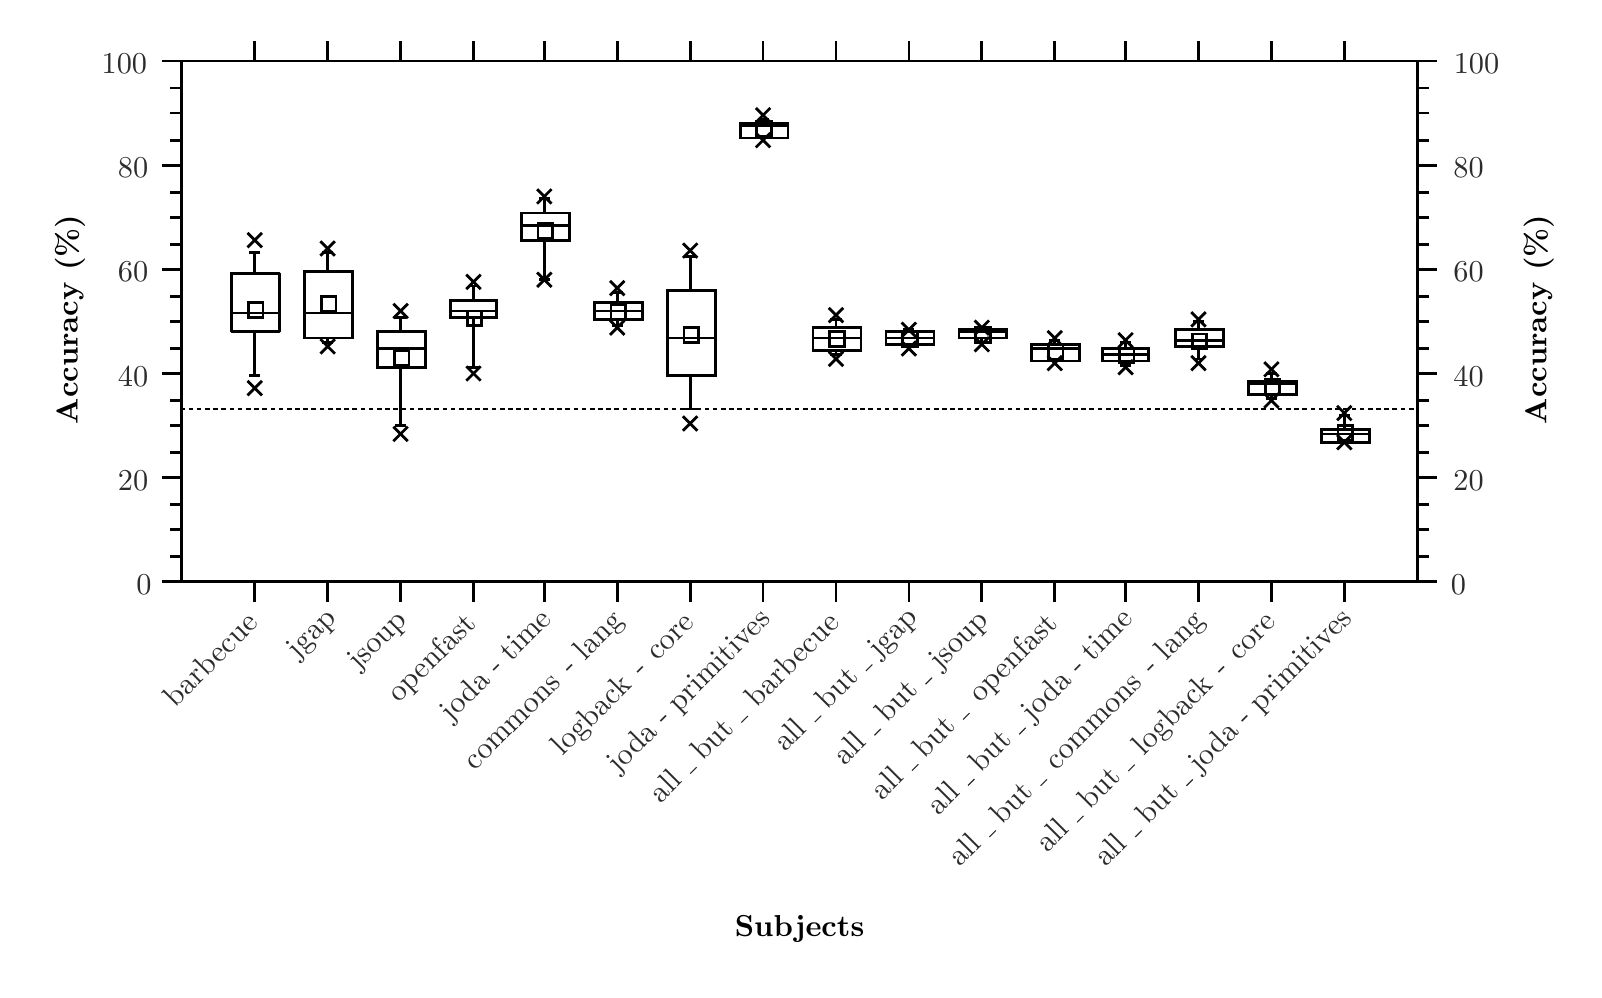
\begin{tikzpicture}{0pt}{0pt}{742pt}{452pt}
	\clip(0pt,452pt) -- (558.587pt,452pt) -- (558.587pt,111.729pt) -- (0pt,111.729pt) -- (0pt,452pt);
\begin{scope}
	\clip(55.7081pt,439.955pt) -- (502.126pt,439.955pt) -- (502.126pt,251.752pt) -- (55.7081pt,251.752pt) -- (55.7081pt,439.955pt);
	\color[rgb]{0,0,0}
	\draw[line width=1pt, line join=bevel, line cap=rect](73.7756pt,363.168pt) -- (91.0903pt,363.168pt) -- (91.0903pt,342.089pt) -- (73.7756pt,342.089pt) -- (73.7756pt,363.168pt);
	\color[rgb]{0,0,0}
	\draw[line width=1pt, line join=bevel, line cap=rect](80.5509pt,326.28pt) -- (83.5622pt,326.28pt);
	\draw[line width=1pt, line join=bevel, line cap=rect](80.5509pt,370.696pt) -- (83.5622pt,370.696pt);
	\draw[line width=1pt, line join=bevel, line cap=rect](82.0566pt,370.696pt) -- (82.0566pt,363.168pt);
	\draw[line width=1pt, line join=bevel, line cap=rect](82.0566pt,326.28pt) -- (82.0566pt,342.089pt);
	\draw[line width=1pt, line join=bevel, line cap=rect](73.7756pt,348.865pt) -- (90.3375pt,348.865pt);
	\draw[line width=1pt, line join=miter, line cap=rect](79.7981pt,324.022pt) -- (84.315pt,319.505pt);
	\draw[line width=1pt, line join=miter, line cap=rect](79.7981pt,319.505pt) -- (84.315pt,324.022pt);
	\draw[line width=1pt, line join=miter, line cap=rect](79.7981pt,377.472pt) -- (84.315pt,372.955pt);
	\draw[line width=1pt, line join=miter, line cap=rect](79.7981pt,372.955pt) -- (84.315pt,377.472pt);
	\draw[line width=1pt, line join=miter, line cap=rect](79.7981pt,352.629pt) -- (85.0678pt,352.629pt) -- (85.0678pt,347.359pt) -- (79.7981pt,347.359pt) -- (79.7981pt,352.629pt);
	\draw[line width=1pt, line join=miter, line cap=rect](100.124pt,363.921pt) -- (117.439pt,363.921pt) -- (117.439pt,339.831pt) -- (100.124pt,339.831pt) -- (100.124pt,363.921pt);
	\draw[line width=1pt, line join=miter, line cap=rect](106.899pt,338.325pt) -- (109.911pt,338.325pt);
	\draw[line width=1pt, line join=miter, line cap=rect](106.899pt,370.696pt) -- (109.911pt,370.696pt);
	\draw[line width=1pt, line join=miter, line cap=rect](108.405pt,370.696pt) -- (108.405pt,363.921pt);
	\draw[line width=1pt, line join=miter, line cap=rect](108.405pt,338.325pt) -- (108.405pt,339.831pt);
	\draw[line width=1pt, line join=miter, line cap=rect](100.124pt,348.865pt) -- (116.686pt,348.865pt);
	\draw[line width=1pt, line join=miter, line cap=rect](106.147pt,339.078pt) -- (110.663pt,334.561pt);
	\draw[line width=1pt, line join=miter, line cap=rect](106.147pt,334.561pt) -- (110.663pt,339.078pt);
	\draw[line width=1pt, line join=miter, line cap=rect](106.147pt,374.46pt) -- (110.663pt,369.943pt);
	\draw[line width=1pt, line join=miter, line cap=rect](106.147pt,369.943pt) -- (110.663pt,374.46pt);
	\draw[line width=1pt, line join=miter, line cap=rect](106.147pt,354.887pt) -- (111.416pt,354.887pt) -- (111.416pt,349.618pt) -- (106.147pt,349.618pt) -- (106.147pt,354.887pt);
	\draw[line width=1pt, line join=miter, line cap=rect](126.472pt,342.089pt) -- (143.787pt,342.089pt) -- (143.787pt,329.292pt) -- (126.472pt,329.292pt) -- (126.472pt,342.089pt);
	\draw[line width=1pt, line join=miter, line cap=rect](133.248pt,308.213pt) -- (136.259pt,308.213pt);
	\draw[line width=1pt, line join=miter, line cap=rect](133.248pt,347.359pt) -- (136.259pt,347.359pt);
	\draw[line width=1pt, line join=miter, line cap=rect](134.753pt,347.359pt) -- (134.753pt,342.089pt);
	\draw[line width=1pt, line join=miter, line cap=rect](134.753pt,308.213pt) -- (134.753pt,329.292pt);
	\draw[line width=1pt, line join=miter, line cap=rect](126.472pt,336.067pt) -- (143.034pt,336.067pt);
	\draw[line width=1pt, line join=miter, line cap=rect](132.495pt,307.46pt) -- (137.012pt,302.943pt);
	\draw[line width=1pt, line join=miter, line cap=rect](132.495pt,302.943pt) -- (137.012pt,307.46pt);
	\draw[line width=1pt, line join=miter, line cap=rect](132.495pt,351.876pt) -- (137.012pt,347.359pt);
	\draw[line width=1pt, line join=miter, line cap=rect](132.495pt,347.359pt) -- (137.012pt,351.876pt);
	\draw[line width=1pt, line join=miter, line cap=rect](132.495pt,335.314pt) -- (137.765pt,335.314pt) -- (137.765pt,330.044pt) -- (132.495pt,330.044pt) -- (132.495pt,335.314pt);
	\draw[line width=1pt, line join=miter, line cap=rect](152.821pt,353.382pt) -- (169.383pt,353.382pt) -- (169.383pt,347.359pt) -- (152.821pt,347.359pt) -- (152.821pt,353.382pt);
	\draw[line width=1pt, line join=miter, line cap=rect](159.596pt,329.292pt) -- (162.607pt,329.292pt);
	\draw[line width=1pt, line join=miter, line cap=rect](159.596pt,358.651pt) -- (162.607pt,358.651pt);
	\draw[line width=1pt, line join=miter, line cap=rect](161.102pt,358.651pt) -- (161.102pt,353.382pt);
	\draw[line width=1pt, line join=miter, line cap=rect](161.102pt,329.292pt) -- (161.102pt,347.359pt);
	\draw[line width=1pt, line join=miter, line cap=rect](152.821pt,349.618pt) -- (169.383pt,349.618pt);
	\draw[line width=1pt, line join=miter, line cap=rect](158.843pt,329.292pt) -- (163.36pt,324.775pt);
	\draw[line width=1pt, line join=miter, line cap=rect](158.843pt,324.775pt) -- (163.36pt,329.292pt);
	\draw[line width=1pt, line join=miter, line cap=rect](158.843pt,362.415pt) -- (163.36pt,357.898pt);
	\draw[line width=1pt, line join=miter, line cap=rect](158.843pt,357.898pt) -- (163.36pt,362.415pt);
	\draw[line width=1pt, line join=miter, line cap=rect](158.843pt,349.618pt) -- (164.113pt,349.618pt) -- (164.113pt,344.348pt) -- (158.843pt,344.348pt) -- (158.843pt,349.618pt);
	\draw[line width=1pt, line join=miter, line cap=rect](178.417pt,385pt) -- (195.731pt,385pt) -- (195.731pt,375.213pt) -- (178.417pt,375.213pt) -- (178.417pt,385pt);
	\draw[line width=1pt, line join=miter, line cap=rect](185.192pt,360.91pt) -- (188.203pt,360.91pt);
	\draw[line width=1pt, line join=miter, line cap=rect](185.192pt,390.269pt) -- (188.203pt,390.269pt);
	\draw[line width=1pt, line join=miter, line cap=rect](186.697pt,390.269pt) -- (186.697pt,385pt);
	\draw[line width=1pt, line join=miter, line cap=rect](186.697pt,360.91pt) -- (186.697pt,375.213pt);
	\draw[line width=1pt, line join=miter, line cap=rect](178.417pt,380.483pt) -- (194.978pt,380.483pt);
	\draw[line width=1pt, line join=miter, line cap=rect](184.439pt,363.168pt) -- (188.956pt,358.651pt);
	\draw[line width=1pt, line join=miter, line cap=rect](184.439pt,358.651pt) -- (188.956pt,363.168pt);
	\draw[line width=1pt, line join=miter, line cap=rect](184.439pt,393.281pt) -- (188.956pt,388.764pt);
	\draw[line width=1pt, line join=miter, line cap=rect](184.439pt,388.764pt) -- (188.956pt,393.281pt);
	\draw[line width=1pt, line join=miter, line cap=rect](184.439pt,381.236pt) -- (189.709pt,381.236pt) -- (189.709pt,375.966pt) -- (184.439pt,375.966pt) -- (184.439pt,381.236pt);
	\draw[line width=1pt, line join=miter, line cap=rect](204.765pt,352.629pt) -- (222.08pt,352.629pt) -- (222.08pt,346.606pt) -- (204.765pt,346.606pt) -- (204.765pt,352.629pt);
	\draw[line width=1pt, line join=miter, line cap=rect](211.54pt,344.348pt) -- (214.552pt,344.348pt);
	\draw[line width=1pt, line join=miter, line cap=rect](211.54pt,356.393pt) -- (214.552pt,356.393pt);
	\draw[line width=1pt, line join=miter, line cap=rect](213.046pt,356.393pt) -- (213.046pt,352.629pt);
	\draw[line width=1pt, line join=miter, line cap=rect](213.046pt,344.348pt) -- (213.046pt,346.606pt);
	\draw[line width=1pt, line join=miter, line cap=rect](204.765pt,349.618pt) -- (221.327pt,349.618pt);
	\draw[line width=1pt, line join=miter, line cap=rect](210.787pt,345.853pt) -- (215.304pt,341.337pt);
	\draw[line width=1pt, line join=miter, line cap=rect](210.787pt,341.337pt) -- (215.304pt,345.853pt);
	\draw[line width=1pt, line join=miter, line cap=rect](210.787pt,360.157pt) -- (215.304pt,355.64pt);
	\draw[line width=1pt, line join=miter, line cap=rect](210.787pt,355.64pt) -- (215.304pt,360.157pt);
	\draw[line width=1pt, line join=miter, line cap=rect](210.787pt,351.876pt) -- (216.057pt,351.876pt) -- (216.057pt,346.606pt) -- (210.787pt,346.606pt) -- (210.787pt,351.876pt);
	\draw[line width=1pt, line join=miter, line cap=rect](231.113pt,357.146pt) -- (248.428pt,357.146pt) -- (248.428pt,326.28pt) -- (231.113pt,326.28pt) -- (231.113pt,357.146pt);
	\draw[line width=1pt, line join=miter, line cap=rect](237.889pt,314.235pt) -- (240.9pt,314.235pt);
	\draw[line width=1pt, line join=miter, line cap=rect](237.889pt,369.191pt) -- (240.9pt,369.191pt);
	\draw[line width=1pt, line join=miter, line cap=rect](239.394pt,369.191pt) -- (239.394pt,357.146pt);
	\draw[line width=1pt, line join=miter, line cap=rect](239.394pt,314.235pt) -- (239.394pt,326.28pt);
	\draw[line width=1pt, line join=miter, line cap=rect](231.113pt,339.831pt) -- (247.675pt,339.831pt);
	\draw[line width=1pt, line join=miter, line cap=rect](237.136pt,311.224pt) -- (241.653pt,306.707pt);
	\draw[line width=1pt, line join=miter, line cap=rect](237.136pt,306.707pt) -- (241.653pt,311.224pt);
	\draw[line width=1pt, line join=miter, line cap=rect](237.136pt,373.707pt) -- (241.653pt,369.191pt);
	\draw[line width=1pt, line join=miter, line cap=rect](237.136pt,369.191pt) -- (241.653pt,373.707pt);
	\draw[line width=1pt, line join=miter, line cap=rect](237.136pt,343.595pt) -- (242.406pt,343.595pt) -- (242.406pt,338.325pt) -- (237.136pt,338.325pt) -- (237.136pt,343.595pt);
	\draw[line width=1pt, line join=miter, line cap=rect](257.462pt,417.371pt) -- (274.777pt,417.371pt) -- (274.777pt,412.101pt) -- (257.462pt,412.101pt) -- (257.462pt,417.371pt);
	\draw[line width=1pt, line join=miter, line cap=rect](264.237pt,412.101pt) -- (267.248pt,412.101pt);
	\draw[line width=1pt, line join=miter, line cap=rect](264.237pt,418.876pt) -- (267.248pt,418.876pt);
	\draw[line width=1pt, line join=miter, line cap=rect](265.743pt,418.876pt) -- (265.743pt,417.371pt);

	\draw[line width=1pt, line join=miter, line cap=rect](257.462pt,416.618pt) -- (274.024pt,416.618pt);
	\draw[line width=1pt, line join=miter, line cap=rect](263.484pt,413.607pt) -- (268.001pt,409.09pt);
	\draw[line width=1pt, line join=miter, line cap=rect](263.484pt,409.09pt) -- (268.001pt,413.607pt);
	\draw[line width=1pt, line join=miter, line cap=rect](263.484pt,422.64pt) -- (268.001pt,418.123pt);
	\draw[line width=1pt, line join=miter, line cap=rect](263.484pt,418.123pt) -- (268.001pt,422.64pt);
	\draw[line width=1pt, line join=miter, line cap=rect](263.484pt,418.123pt) -- (268.754pt,418.123pt) -- (268.754pt,412.854pt) -- (263.484pt,412.854pt) -- (263.484pt,418.123pt);
	\draw[line width=1pt, line join=miter, line cap=rect](283.81pt,343.595pt) -- (301.125pt,343.595pt) -- (301.125pt,335.314pt) -- (283.81pt,335.314pt) -- (283.81pt,343.595pt);
	\draw[line width=1pt, line join=miter, line cap=rect](290.586pt,333.808pt) -- (293.597pt,333.808pt);
	\draw[line width=1pt, line join=miter, line cap=rect](290.586pt,346.606pt) -- (293.597pt,346.606pt);
	\draw[line width=1pt, line join=miter, line cap=rect](292.091pt,346.606pt) -- (292.091pt,343.595pt);
	\draw[line width=1pt, line join=miter, line cap=rect](292.091pt,333.808pt) -- (292.091pt,335.314pt);
	\draw[line width=1pt, line join=miter, line cap=rect](283.81pt,339.831pt) -- (300.372pt,339.831pt);
	\draw[line width=1pt, line join=miter, line cap=rect](289.833pt,334.561pt) -- (294.35pt,330.044pt);
	\draw[line width=1pt, line join=miter, line cap=rect](289.833pt,330.044pt) -- (294.35pt,334.561pt);
	\draw[line width=1pt, line join=miter, line cap=rect](289.833pt,350.37pt) -- (294.35pt,345.853pt);
	\draw[line width=1pt, line join=miter, line cap=rect](289.833pt,345.853pt) -- (294.35pt,350.37pt);
	\draw[line width=1pt, line join=miter, line cap=rect](289.833pt,342.089pt) -- (295.103pt,342.089pt) -- (295.103pt,336.82pt) -- (289.833pt,336.82pt) -- (289.833pt,342.089pt);
	\draw[line width=1pt, line join=miter, line cap=rect](310.159pt,342.089pt) -- (327.473pt,342.089pt) -- (327.473pt,337.572pt) -- (310.159pt,337.572pt) -- (310.159pt,342.089pt);
	\draw[line width=1pt, line join=miter, line cap=rect](316.934pt,336.82pt) -- (319.945pt,336.82pt);
	\draw[line width=1pt, line join=miter, line cap=rect](316.934pt,342.842pt) -- (319.945pt,342.842pt);
	\draw[line width=1pt, line join=miter, line cap=rect](318.44pt,342.842pt) -- (318.44pt,342.089pt);
	\draw[line width=1pt, line join=miter, line cap=rect](318.44pt,336.82pt) -- (318.44pt,337.572pt);
	\draw[line width=1pt, line join=miter, line cap=rect](310.159pt,339.831pt) -- (326.721pt,339.831pt);
	\draw[line width=1pt, line join=miter, line cap=rect](316.181pt,338.325pt) -- (320.698pt,333.808pt);
	\draw[line width=1pt, line join=miter, line cap=rect](316.181pt,333.808pt) -- (320.698pt,338.325pt);
	\draw[line width=1pt, line join=miter, line cap=rect](316.181pt,345.101pt) -- (320.698pt,340.584pt);
	\draw[line width=1pt, line join=miter, line cap=rect](316.181pt,340.584pt) -- (320.698pt,345.101pt);
	\draw[line width=1pt, line join=miter, line cap=rect](316.181pt,342.089pt) -- (321.451pt,342.089pt) -- (321.451pt,336.82pt) -- (316.181pt,336.82pt) -- (316.181pt,342.089pt);
	\draw[line width=1pt, line join=miter, line cap=rect](336.507pt,342.842pt) -- (353.822pt,342.842pt) -- (353.822pt,339.831pt) -- (336.507pt,339.831pt) -- (336.507pt,342.842pt);
	\draw[line width=1pt, line join=miter, line cap=rect](343.282pt,338.325pt) -- (346.294pt,338.325pt);
	\draw[line width=1pt, line join=miter, line cap=rect](343.282pt,343.595pt) -- (346.294pt,343.595pt);
	\draw[line width=1pt, line join=miter, line cap=rect](344.788pt,343.595pt) -- (344.788pt,342.842pt);
	\draw[line width=1pt, line join=miter, line cap=rect](344.788pt,338.325pt) -- (344.788pt,339.831pt);
	\draw[line width=1pt, line join=miter, line cap=rect](336.507pt,342.089pt) -- (353.069pt,342.089pt);
	\draw[line width=1pt, line join=miter, line cap=rect](342.53pt,339.831pt) -- (347.047pt,335.314pt);
	\draw[line width=1pt, line join=miter, line cap=rect](342.53pt,335.314pt) -- (347.047pt,339.831pt);
	\draw[line width=1pt, line join=miter, line cap=rect](342.53pt,345.853pt) -- (347.047pt,341.337pt);
	\draw[line width=1pt, line join=miter, line cap=rect](342.53pt,341.337pt) -- (347.047pt,345.853pt);
	\draw[line width=1pt, line join=miter, line cap=rect](342.53pt,343.595pt) -- (347.799pt,343.595pt) -- (347.799pt,338.325pt) -- (342.53pt,338.325pt) -- (342.53pt,343.595pt);
	\draw[line width=1pt, line join=miter, line cap=rect](362.856pt,337.572pt) -- (380.17pt,337.572pt) -- (380.17pt,331.55pt) -- (362.856pt,331.55pt) -- (362.856pt,337.572pt);
	\draw[line width=1pt, line join=miter, line cap=rect](369.631pt,331.55pt) -- (372.642pt,331.55pt);
	\draw[line width=1pt, line join=miter, line cap=rect](369.631pt,339.078pt) -- (372.642pt,339.078pt);
	\draw[line width=1pt, line join=miter, line cap=rect](371.137pt,339.078pt) -- (371.137pt,337.572pt);

	\draw[line width=1pt, line join=miter, line cap=rect](362.856pt,336.067pt) -- (379.418pt,336.067pt);
	\draw[line width=1pt, line join=miter, line cap=rect](368.878pt,333.056pt) -- (373.395pt,328.539pt);
	\draw[line width=1pt, line join=miter, line cap=rect](368.878pt,328.539pt) -- (373.395pt,333.056pt);
	\draw[line width=1pt, line join=miter, line cap=rect](368.878pt,342.089pt) -- (373.395pt,337.572pt);
	\draw[line width=1pt, line join=miter, line cap=rect](368.878pt,337.572pt) -- (373.395pt,342.089pt);
	\draw[line width=1pt, line join=miter, line cap=rect](368.878pt,337.572pt) -- (374.148pt,337.572pt) -- (374.148pt,332.303pt) -- (368.878pt,332.303pt) -- (368.878pt,337.572pt);
	\draw[line width=1pt, line join=miter, line cap=rect](388.451pt,336.067pt) -- (405.013pt,336.067pt) -- (405.013pt,331.55pt) -- (388.451pt,331.55pt) -- (388.451pt,336.067pt);
	\draw[line width=1pt, line join=miter, line cap=rect](395.227pt,330.044pt) -- (398.238pt,330.044pt);
	\draw[line width=1pt, line join=miter, line cap=rect](395.227pt,338.325pt) -- (398.238pt,338.325pt);
	\draw[line width=1pt, line join=miter, line cap=rect](396.732pt,338.325pt) -- (396.732pt,336.067pt);
	\draw[line width=1pt, line join=miter, line cap=rect](396.732pt,330.044pt) -- (396.732pt,331.55pt);
	\draw[line width=1pt, line join=miter, line cap=rect](388.451pt,333.808pt) -- (405.013pt,333.808pt);
	\draw[line width=1pt, line join=miter, line cap=rect](394.474pt,331.55pt) -- (398.991pt,327.033pt);
	\draw[line width=1pt, line join=miter, line cap=rect](394.474pt,327.033pt) -- (398.991pt,331.55pt);
	\draw[line width=1pt, line join=miter, line cap=rect](394.474pt,341.337pt) -- (398.991pt,336.82pt);
	\draw[line width=1pt, line join=miter, line cap=rect](394.474pt,336.82pt) -- (398.991pt,341.337pt);
	\draw[line width=1pt, line join=miter, line cap=rect](394.474pt,336.067pt) -- (399.743pt,336.067pt) -- (399.743pt,330.797pt) -- (394.474pt,330.797pt) -- (394.474pt,336.067pt);
	\draw[line width=1pt, line join=miter, line cap=rect](414.8pt,342.842pt) -- (432.114pt,342.842pt) -- (432.114pt,336.82pt) -- (414.8pt,336.82pt) -- (414.8pt,342.842pt);
	\draw[line width=1pt, line join=miter, line cap=rect](421.575pt,332.303pt) -- (424.586pt,332.303pt);
	\draw[line width=1pt, line join=miter, line cap=rect](421.575pt,345.853pt) -- (424.586pt,345.853pt);
	\draw[line width=1pt, line join=miter, line cap=rect](423.081pt,345.853pt) -- (423.081pt,342.842pt);
	\draw[line width=1pt, line join=miter, line cap=rect](423.081pt,332.303pt) -- (423.081pt,336.82pt);
	\draw[line width=1pt, line join=miter, line cap=rect](414.8pt,339.078pt) -- (431.362pt,339.078pt);
	\draw[line width=1pt, line join=miter, line cap=rect](420.822pt,333.056pt) -- (425.339pt,328.539pt);
	\draw[line width=1pt, line join=miter, line cap=rect](420.822pt,328.539pt) -- (425.339pt,333.056pt);
	\draw[line width=1pt, line join=miter, line cap=rect](420.822pt,348.865pt) -- (425.339pt,344.348pt);
	\draw[line width=1pt, line join=miter, line cap=rect](420.822pt,344.348pt) -- (425.339pt,348.865pt);
	\draw[line width=1pt, line join=miter, line cap=rect](420.822pt,341.337pt) -- (426.092pt,341.337pt) -- (426.092pt,336.067pt) -- (420.822pt,336.067pt) -- (420.822pt,341.337pt);
	\draw[line width=1pt, line join=miter, line cap=rect](441.148pt,324.022pt) -- (458.463pt,324.022pt) -- (458.463pt,319.505pt) -- (441.148pt,319.505pt) -- (441.148pt,324.022pt);
	\draw[line width=1pt, line join=miter, line cap=rect](447.923pt,317.999pt) -- (450.935pt,317.999pt);
	\draw[line width=1pt, line join=miter, line cap=rect](447.923pt,327.033pt) -- (450.935pt,327.033pt);
	\draw[line width=1pt, line join=miter, line cap=rect](449.429pt,327.033pt) -- (449.429pt,324.022pt);
	\draw[line width=1pt, line join=miter, line cap=rect](449.429pt,317.999pt) -- (449.429pt,319.505pt);
	\draw[line width=1pt, line join=miter, line cap=rect](441.148pt,323.269pt) -- (457.71pt,323.269pt);
	\draw[line width=1pt, line join=miter, line cap=rect](447.171pt,319.505pt) -- (451.688pt,314.988pt);
	\draw[line width=1pt, line join=miter, line cap=rect](447.171pt,314.988pt) -- (451.688pt,319.505pt);
	\draw[line width=1pt, line join=miter, line cap=rect](447.171pt,330.797pt) -- (451.688pt,326.28pt);
	\draw[line width=1pt, line join=miter, line cap=rect](447.171pt,326.28pt) -- (451.688pt,330.797pt);
	\draw[line width=1pt, line join=miter, line cap=rect](447.171pt,324.775pt) -- (452.44pt,324.775pt) -- (452.44pt,319.505pt) -- (447.171pt,319.505pt) -- (447.171pt,324.775pt);
	\draw[line width=1pt, line join=miter, line cap=rect](467.497pt,306.707pt) -- (484.811pt,306.707pt) -- (484.811pt,302.19pt) -- (467.497pt,302.19pt) -- (467.497pt,306.707pt);
	\draw[line width=1pt, line join=miter, line cap=rect](474.272pt,302.19pt) -- (477.283pt,302.19pt);
	\draw[line width=1pt, line join=miter, line cap=rect](474.272pt,311.977pt) -- (477.283pt,311.977pt);
	\draw[line width=1pt, line join=miter, line cap=rect](475.777pt,311.977pt) -- (475.777pt,306.707pt);

	\draw[line width=1pt, line join=miter, line cap=rect](467.497pt,305.202pt) -- (484.058pt,305.202pt);
	\draw[line width=1pt, line join=miter, line cap=rect](473.519pt,304.449pt) -- (478.036pt,299.932pt);
	\draw[line width=1pt, line join=miter, line cap=rect](473.519pt,299.932pt) -- (478.036pt,304.449pt);
	\draw[line width=1pt, line join=miter, line cap=rect](473.519pt,314.988pt) -- (478.036pt,310.471pt);
	\draw[line width=1pt, line join=miter, line cap=rect](473.519pt,310.471pt) -- (478.036pt,314.988pt);
	\draw[line width=1pt, line join=miter, line cap=rect](473.519pt,308.213pt) -- (478.789pt,308.213pt) -- (478.789pt,302.943pt) -- (473.519pt,302.943pt) -- (473.519pt,308.213pt);


	\draw[line width=1pt, dash pattern=on 0.024cm off 0.08cm, dash phase=0pt, line join=miter, line cap=rect](55.7081pt,314.235pt) -- (528.474pt,314.235pt);
\end{scope}
\begin{scope}
	\color[rgb]{0,0,0}
	\pgftext[center, base, at={\pgfpoint{18.0675pt}{346.606pt}},rotate=90]{\fontsize{11}{0}\selectfont{\textbf{Accuracy (\%)}}}
	\color[rgb]{0.172549,0.172549,0.172549}
	\pgftext[center, base, at={\pgfpoint{42.0163pt}{247.235pt}}]{\fontsize{11}{0}\selectfont{0}}
	\pgftext[center, base, at={\pgfpoint{38.1111pt}{284.876pt}}]{\fontsize{11}{0}\selectfont{20}}
	\pgftext[center, base, at={\pgfpoint{38.1111pt}{322.516pt}}]{\fontsize{11}{0}\selectfont{40}}
	\pgftext[center, base, at={\pgfpoint{38.1111pt}{360.157pt}}]{\fontsize{11}{0}\selectfont{60}}
	\pgftext[center, base, at={\pgfpoint{38.1111pt}{397.798pt}}]{\fontsize{11}{0}\selectfont{80}}
	\pgftext[center, base, at={\pgfpoint{34.9587pt}{435.438pt}}]{\fontsize{11}{0}\selectfont{100}}
	\color[rgb]{0,0,0}
	\draw[line width=1pt, line join=bevel, line cap=rect](55.7081pt,260.786pt) -- (51.9441pt,260.786pt);
	\draw[line width=1pt, line join=bevel, line cap=rect](55.7081pt,279.606pt) -- (51.9441pt,279.606pt);
	\draw[line width=1pt, line join=bevel, line cap=rect](55.7081pt,298.426pt) -- (51.9441pt,298.426pt);
	\draw[line width=1pt, line join=bevel, line cap=rect](55.7081pt,317.247pt) -- (51.9441pt,317.247pt);
	\draw[line width=1pt, line join=bevel, line cap=rect](55.7081pt,336.067pt) -- (51.9441pt,336.067pt);
	\draw[line width=1pt, line join=bevel, line cap=rect](55.7081pt,354.887pt) -- (51.9441pt,354.887pt);
	\draw[line width=1pt, line join=bevel, line cap=rect](55.7081pt,373.707pt) -- (51.9441pt,373.707pt);
	\draw[line width=1pt, line join=bevel, line cap=rect](55.7081pt,392.528pt) -- (51.9441pt,392.528pt);
	\draw[line width=1pt, line join=bevel, line cap=rect](55.7081pt,411.348pt) -- (51.9441pt,411.348pt);
	\draw[line width=1pt, line join=bevel, line cap=rect](55.7081pt,430.168pt) -- (51.9441pt,430.168pt);
	\draw[line width=1pt, line join=bevel, line cap=rect](55.7081pt,270.572pt) -- (51.9441pt,270.572pt);
	\draw[line width=1pt, line join=bevel, line cap=rect](55.7081pt,308.213pt) -- (51.9441pt,308.213pt);
	\draw[line width=1pt, line join=bevel, line cap=rect](55.7081pt,345.853pt) -- (51.9441pt,345.853pt);
	\draw[line width=1pt, line join=bevel, line cap=rect](55.7081pt,383.494pt) -- (51.9441pt,383.494pt);
	\draw[line width=1pt, line join=bevel, line cap=rect](55.7081pt,421.135pt) -- (51.9441pt,421.135pt);
	\draw[line width=1pt, line join=bevel, line cap=rect](55.7081pt,251.752pt) -- (48.9328pt,251.752pt);
	\draw[line width=1pt, line join=bevel, line cap=rect](55.7081pt,289.393pt) -- (48.9328pt,289.393pt);
	\draw[line width=1pt, line join=bevel, line cap=rect](55.7081pt,327.033pt) -- (48.9328pt,327.033pt);
	\draw[line width=1pt, line join=bevel, line cap=rect](55.7081pt,364.674pt) -- (48.9328pt,364.674pt);
	\draw[line width=1pt, line join=bevel, line cap=rect](55.7081pt,402.314pt) -- (48.9328pt,402.314pt);
	\draw[line width=1pt, line join=bevel, line cap=rect](55.7081pt,439.955pt) -- (48.9328pt,439.955pt);
	\draw[line width=1pt, line join=bevel, line cap=rect](55.7081pt,439.955pt) -- (55.7081pt,251.752pt);
	\pgftext[center, base, at={\pgfpoint{548.8pt}{346.606pt}},rotate=90]{\fontsize{11}{0}\selectfont{\textbf{Accuracy (\%)}}}
	\color[rgb]{0.172549,0.172549,0.172549}
	\pgftext[center, base, at={\pgfpoint{517.041pt}{247.235pt}}]{\fontsize{11}{0}\selectfont{0}}
	\pgftext[center, base, at={\pgfpoint{520.664pt}{284.876pt}}]{\fontsize{11}{0}\selectfont{20}}
	\pgftext[center, base, at={\pgfpoint{520.664pt}{322.516pt}}]{\fontsize{11}{0}\selectfont{40}}
	\pgftext[center, base, at={\pgfpoint{520.664pt}{360.157pt}}]{\fontsize{11}{0}\selectfont{60}}
	\pgftext[center, base, at={\pgfpoint{520.664pt}{397.798pt}}]{\fontsize{11}{0}\selectfont{80}}
	\pgftext[center, base, at={\pgfpoint{523.534pt}{435.438pt}}]{\fontsize{11}{0}\selectfont{100}}
	\color[rgb]{0,0,0}
	\draw[line width=1pt, line join=bevel, line cap=rect](502.126pt,260.786pt) -- (505.89pt,260.786pt);
	\draw[line width=1pt, line join=bevel, line cap=rect](502.126pt,279.606pt) -- (505.89pt,279.606pt);
	\draw[line width=1pt, line join=bevel, line cap=rect](502.126pt,298.426pt) -- (505.89pt,298.426pt);
	\draw[line width=1pt, line join=bevel, line cap=rect](502.126pt,317.247pt) -- (505.89pt,317.247pt);
	\draw[line width=1pt, line join=bevel, line cap=rect](502.126pt,336.067pt) -- (505.89pt,336.067pt);
	\draw[line width=1pt, line join=bevel, line cap=rect](502.126pt,354.887pt) -- (505.89pt,354.887pt);
	\draw[line width=1pt, line join=bevel, line cap=rect](502.126pt,373.707pt) -- (505.89pt,373.707pt);
	\draw[line width=1pt, line join=bevel, line cap=rect](502.126pt,392.528pt) -- (505.89pt,392.528pt);
	\draw[line width=1pt, line join=bevel, line cap=rect](502.126pt,411.348pt) -- (505.89pt,411.348pt);
	\draw[line width=1pt, line join=bevel, line cap=rect](502.126pt,430.168pt) -- (505.89pt,430.168pt);
	\draw[line width=1pt, line join=bevel, line cap=rect](502.126pt,270.572pt) -- (505.89pt,270.572pt);
	\draw[line width=1pt, line join=bevel, line cap=rect](502.126pt,308.213pt) -- (505.89pt,308.213pt);
	\draw[line width=1pt, line join=bevel, line cap=rect](502.126pt,345.853pt) -- (505.89pt,345.853pt);
	\draw[line width=1pt, line join=bevel, line cap=rect](502.126pt,383.494pt) -- (505.89pt,383.494pt);
	\draw[line width=1pt, line join=bevel, line cap=rect](502.126pt,421.135pt) -- (505.89pt,421.135pt);
	\draw[line width=1pt, line join=bevel, line cap=rect](502.126pt,251.752pt) -- (508.901pt,251.752pt);
	\draw[line width=1pt, line join=bevel, line cap=rect](502.126pt,289.393pt) -- (508.901pt,289.393pt);
	\draw[line width=1pt, line join=bevel, line cap=rect](502.126pt,327.033pt) -- (508.901pt,327.033pt);
	\draw[line width=1pt, line join=bevel, line cap=rect](502.126pt,364.674pt) -- (508.901pt,364.674pt);
	\draw[line width=1pt, line join=bevel, line cap=rect](502.126pt,402.314pt) -- (508.901pt,402.314pt);
	\draw[line width=1pt, line join=bevel, line cap=rect](502.126pt,439.955pt) -- (508.901pt,439.955pt);
	\draw[line width=1pt, line join=bevel, line cap=rect](502.126pt,439.955pt) -- (502.126pt,251.752pt);
	\pgftext[center, base, at={\pgfpoint{278.917pt}{123.774pt}}]{\fontsize{11}{0}\selectfont{\textbf{Subjects}}}
	\color[rgb]{0.172549,0.172549,0.172549}
	\pgftext[center, base, at={\pgfpoint{68.4991pt}{221.267pt}},rotate=45]{\fontsize{11}{0}\selectfont{barbecue}}
	\pgftext[center, base, at={\pgfpoint{104.654pt}{231.073pt}},rotate=45]{\fontsize{11}{0}\selectfont{jgap}}
	\pgftext[center, base, at={\pgfpoint{128.445pt}{228.516pt}},rotate=45]{\fontsize{11}{0}\selectfont{jsoup}}
	\pgftext[center, base, at={\pgfpoint{148.222pt}{221.945pt}},rotate=45]{\fontsize{11}{0}\selectfont{openfast}}
	\pgftext[center, base, at={\pgfpoint{160.198pt}{208.325pt}},rotate=45]{\fontsize{11}{0}\selectfont{joda}}
	\pgftext[center, base, at={\pgfpoint{171.111pt}{219.238pt}},rotate=45]{\fontsize{11}{0}\selectfont{-}}
	\pgftext[center, base, at={\pgfpoint{182.11pt}{230.238pt}},rotate=45]{\fontsize{11}{0}\selectfont{time}}
	\pgftext[center, base, at={\pgfpoint{177.272pt}{199.051pt}},rotate=45]{\fontsize{11}{0}\selectfont{commons}}
	\pgftext[center, base, at={\pgfpoint{197.542pt}{219.321pt}},rotate=45]{\fontsize{11}{0}\selectfont{-}}
	\pgftext[center, base, at={\pgfpoint{208.405pt}{230.184pt}},rotate=45]{\fontsize{11}{0}\selectfont{lang}}
	\pgftext[center, base, at={\pgfpoint{205.896pt}{201.326pt}},rotate=45]{\fontsize{11}{0}\selectfont{logback}}
	\pgftext[center, base, at={\pgfpoint{223.117pt}{218.547pt}},rotate=45]{\fontsize{11}{0}\selectfont{-}}
	\pgftext[center, base, at={\pgfpoint{234.342pt}{229.772pt}},rotate=45]{\fontsize{11}{0}\selectfont{core}}
	\pgftext[center, base, at={\pgfpoint{220.612pt}{189.694pt}},rotate=45]{\fontsize{11}{0}\selectfont{joda}}
	\pgftext[center, base, at={\pgfpoint{231.525pt}{200.607pt}},rotate=45]{\fontsize{11}{0}\selectfont{-}}
	\pgftext[center, base, at={\pgfpoint{252.027pt}{221.109pt}},rotate=45]{\fontsize{11}{0}\selectfont{primitives}}
	\pgftext[center, base, at={\pgfpoint{232.684pt}{175.417pt}},rotate=45]{\fontsize{11}{0}\selectfont{all}}
	\pgftext[center, base, at={\pgfpoint{240.498pt}{183.231pt}},rotate=45]{\fontsize{11}{0}\selectfont{\_}}
	\pgftext[center, base, at={\pgfpoint{249.743pt}{192.476pt}},rotate=45]{\fontsize{11}{0}\selectfont{but}}
	\pgftext[center, base, at={\pgfpoint{258.988pt}{201.721pt}},rotate=45]{\fontsize{11}{0}\selectfont{\_}}
	\pgftext[center, base, at={\pgfpoint{278.584pt}{221.317pt}},rotate=45]{\fontsize{11}{0}\selectfont{barbecue}}
	\pgftext[center, base, at={\pgfpoint{277.663pt}{194.048pt}},rotate=45]{\fontsize{11}{0}\selectfont{all}}
	\pgftext[center, base, at={\pgfpoint{285.478pt}{201.862pt}},rotate=45]{\fontsize{11}{0}\selectfont{\_}}
	\pgftext[center, base, at={\pgfpoint{294.722pt}{211.107pt}},rotate=45]{\fontsize{11}{0}\selectfont{but}}
	\pgftext[center, base, at={\pgfpoint{303.967pt}{220.352pt}},rotate=45]{\fontsize{11}{0}\selectfont{\_}}
	\pgftext[center, base, at={\pgfpoint{314.738pt}{231.123pt}},rotate=45]{\fontsize{11}{0}\selectfont{jgap}}
	\pgftext[center, base, at={\pgfpoint{299.221pt}{189.257pt}},rotate=45]{\fontsize{11}{0}\selectfont{all}}
	\pgftext[center, base, at={\pgfpoint{307.035pt}{197.072pt}},rotate=45]{\fontsize{11}{0}\selectfont{\_}}
	\pgftext[center, base, at={\pgfpoint{316.28pt}{206.317pt}},rotate=45]{\fontsize{11}{0}\selectfont{but}}
	\pgftext[center, base, at={\pgfpoint{325.525pt}{215.561pt}},rotate=45]{\fontsize{11}{0}\selectfont{\_}}
	\pgftext[center, base, at={\pgfpoint{338.529pt}{228.566pt}},rotate=45]{\fontsize{11}{0}\selectfont{jsoup}}
	\pgftext[center, base, at={\pgfpoint{312.794pt}{176.482pt}},rotate=45]{\fontsize{11}{0}\selectfont{all}}
	\pgftext[center, base, at={\pgfpoint{320.608pt}{184.296pt}},rotate=45]{\fontsize{11}{0}\selectfont{\_}}
	\pgftext[center, base, at={\pgfpoint{329.853pt}{193.541pt}},rotate=45]{\fontsize{11}{0}\selectfont{but}}
	\pgftext[center, base, at={\pgfpoint{339.098pt}{202.786pt}},rotate=45]{\fontsize{11}{0}\selectfont{\_}}
	\pgftext[center, base, at={\pgfpoint{358.307pt}{221.995pt}},rotate=45]{\fontsize{11}{0}\selectfont{openfast}}
	\pgftext[center, base, at={\pgfpoint{333.066pt}{171.159pt}},rotate=45]{\fontsize{11}{0}\selectfont{all}}
	\pgftext[center, base, at={\pgfpoint{340.88pt}{178.973pt}},rotate=45]{\fontsize{11}{0}\selectfont{\_}}
	\pgftext[center, base, at={\pgfpoint{350.125pt}{188.218pt}},rotate=45]{\fontsize{11}{0}\selectfont{but}}
	\pgftext[center, base, at={\pgfpoint{359.37pt}{197.463pt}},rotate=45]{\fontsize{11}{0}\selectfont{\_}}
	\pgftext[center, base, at={\pgfpoint{370.283pt}{208.375pt}},rotate=45]{\fontsize{11}{0}\selectfont{joda}}
	\pgftext[center, base, at={\pgfpoint{381.195pt}{219.288pt}},rotate=45]{\fontsize{11}{0}\selectfont{-}}
	\pgftext[center, base, at={\pgfpoint{392.195pt}{230.287pt}},rotate=45]{\fontsize{11}{0}\selectfont{time}}
	\pgftext[center, base, at={\pgfpoint{340.783pt}{152.527pt}},rotate=45]{\fontsize{11}{0}\selectfont{all}}
	\pgftext[center, base, at={\pgfpoint{348.598pt}{160.342pt}},rotate=45]{\fontsize{11}{0}\selectfont{\_}}
	\pgftext[center, base, at={\pgfpoint{357.842pt}{169.587pt}},rotate=45]{\fontsize{11}{0}\selectfont{but}}
	\pgftext[center, base, at={\pgfpoint{367.087pt}{178.831pt}},rotate=45]{\fontsize{11}{0}\selectfont{\_}}
	\pgftext[center, base, at={\pgfpoint{387.357pt}{199.101pt}},rotate=45]{\fontsize{11}{0}\selectfont{commons}}
	\pgftext[center, base, at={\pgfpoint{407.627pt}{219.371pt}},rotate=45]{\fontsize{11}{0}\selectfont{-}}
	\pgftext[center, base, at={\pgfpoint{418.489pt}{230.233pt}},rotate=45]{\fontsize{11}{0}\selectfont{lang}}
	\pgftext[center, base, at={\pgfpoint{372.455pt}{157.851pt}},rotate=45]{\fontsize{11}{0}\selectfont{all}}
	\pgftext[center, base, at={\pgfpoint{380.269pt}{165.665pt}},rotate=45]{\fontsize{11}{0}\selectfont{\_}}
	\pgftext[center, base, at={\pgfpoint{389.514pt}{174.91pt}},rotate=45]{\fontsize{11}{0}\selectfont{but}}
	\pgftext[center, base, at={\pgfpoint{398.759pt}{184.155pt}},rotate=45]{\fontsize{11}{0}\selectfont{\_}}
	\pgftext[center, base, at={\pgfpoint{415.98pt}{201.376pt}},rotate=45]{\fontsize{11}{0}\selectfont{logback}}
	\pgftext[center, base, at={\pgfpoint{433.202pt}{218.597pt}},rotate=45]{\fontsize{11}{0}\selectfont{-}}
	\pgftext[center, base, at={\pgfpoint{444.426pt}{229.822pt}},rotate=45]{\fontsize{11}{0}\selectfont{core}}
	\pgftext[center, base, at={\pgfpoint{393.48pt}{152.527pt}},rotate=45]{\fontsize{11}{0}\selectfont{all}}
	\pgftext[center, base, at={\pgfpoint{401.294pt}{160.342pt}},rotate=45]{\fontsize{11}{0}\selectfont{\_}}
	\pgftext[center, base, at={\pgfpoint{410.539pt}{169.587pt}},rotate=45]{\fontsize{11}{0}\selectfont{but}}
	\pgftext[center, base, at={\pgfpoint{419.784pt}{178.831pt}},rotate=45]{\fontsize{11}{0}\selectfont{\_}}
	\pgftext[center, base, at={\pgfpoint{430.697pt}{189.744pt}},rotate=45]{\fontsize{11}{0}\selectfont{joda}}
	\pgftext[center, base, at={\pgfpoint{441.609pt}{200.656pt}},rotate=45]{\fontsize{11}{0}\selectfont{-}}
	\pgftext[center, base, at={\pgfpoint{462.112pt}{221.159pt}},rotate=45]{\fontsize{11}{0}\selectfont{primitives}}
	\color[rgb]{0,0,0}
	\draw[line width=1pt, line join=bevel, line cap=rect](82.0566pt,251.752pt) -- (82.0566pt,244.977pt);
	\draw[line width=1pt, line join=bevel, line cap=rect](108.405pt,251.752pt) -- (108.405pt,244.977pt);
	\draw[line width=1pt, line join=bevel, line cap=rect](134.753pt,251.752pt) -- (134.753pt,244.977pt);
	\draw[line width=1pt, line join=bevel, line cap=rect](161.102pt,251.752pt) -- (161.102pt,244.977pt);
	\draw[line width=1pt, line join=bevel, line cap=rect](186.697pt,251.752pt) -- (186.697pt,244.977pt);
	\draw[line width=1pt, line join=bevel, line cap=rect](213.046pt,251.752pt) -- (213.046pt,244.977pt);
	\draw[line width=1pt, line join=bevel, line cap=rect](239.394pt,251.752pt) -- (239.394pt,244.977pt);
	\draw[line width=1pt, line join=bevel, line cap=rect](265.743pt,251.752pt) -- (265.743pt,244.977pt);
	\draw[line width=1pt, line join=bevel, line cap=rect](292.091pt,251.752pt) -- (292.091pt,244.977pt);
	\draw[line width=1pt, line join=bevel, line cap=rect](318.44pt,251.752pt) -- (318.44pt,244.977pt);
	\draw[line width=1pt, line join=bevel, line cap=rect](344.788pt,251.752pt) -- (344.788pt,244.977pt);
	\draw[line width=1pt, line join=bevel, line cap=rect](371.137pt,251.752pt) -- (371.137pt,244.977pt);
	\draw[line width=1pt, line join=bevel, line cap=rect](396.732pt,251.752pt) -- (396.732pt,244.977pt);
	\draw[line width=1pt, line join=bevel, line cap=rect](423.081pt,251.752pt) -- (423.081pt,244.977pt);
	\draw[line width=1pt, line join=bevel, line cap=rect](449.429pt,251.752pt) -- (449.429pt,244.977pt);
	\draw[line width=1pt, line join=bevel, line cap=rect](475.777pt,251.752pt) -- (475.777pt,244.977pt);
	\draw[line width=1pt, line join=bevel, line cap=rect](55.7081pt,251.752pt) -- (502.126pt,251.752pt);
	\draw[line width=1pt, line join=bevel, line cap=rect](82.0566pt,439.955pt) -- (82.0566pt,446.73pt);
	\draw[line width=1pt, line join=bevel, line cap=rect](108.405pt,439.955pt) -- (108.405pt,446.73pt);
	\draw[line width=1pt, line join=bevel, line cap=rect](134.753pt,439.955pt) -- (134.753pt,446.73pt);
	\draw[line width=1pt, line join=bevel, line cap=rect](161.102pt,439.955pt) -- (161.102pt,446.73pt);
	\draw[line width=1pt, line join=bevel, line cap=rect](186.697pt,439.955pt) -- (186.697pt,446.73pt);
	\draw[line width=1pt, line join=bevel, line cap=rect](213.046pt,439.955pt) -- (213.046pt,446.73pt);
	\draw[line width=1pt, line join=bevel, line cap=rect](239.394pt,439.955pt) -- (239.394pt,446.73pt);
	\draw[line width=1pt, line join=bevel, line cap=rect](265.743pt,439.955pt) -- (265.743pt,446.73pt);
	\draw[line width=1pt, line join=bevel, line cap=rect](292.091pt,439.955pt) -- (292.091pt,446.73pt);
	\draw[line width=1pt, line join=bevel, line cap=rect](318.44pt,439.955pt) -- (318.44pt,446.73pt);
	\draw[line width=1pt, line join=bevel, line cap=rect](344.788pt,439.955pt) -- (344.788pt,446.73pt);
	\draw[line width=1pt, line join=bevel, line cap=rect](371.137pt,439.955pt) -- (371.137pt,446.73pt);
	\draw[line width=1pt, line join=bevel, line cap=rect](396.732pt,439.955pt) -- (396.732pt,446.73pt);
	\draw[line width=1pt, line join=bevel, line cap=rect](423.081pt,439.955pt) -- (423.081pt,446.73pt);
	\draw[line width=1pt, line join=bevel, line cap=rect](449.429pt,439.955pt) -- (449.429pt,446.73pt);
	\draw[line width=1pt, line join=bevel, line cap=rect](475.777pt,439.955pt) -- (475.777pt,446.73pt);
	\draw[line width=1pt, line join=bevel, line cap=rect](55.7081pt,439.955pt) -- (502.126pt,439.955pt);
\end{scope}
\end{tikzpicture}

  \end{adjustbox}
  \caption{Method-level training and prediction accuracy over the 8 subjects and sets of \emph{all\_but\_<subject>} using generalized parameters [\emph{cost}=100, \emph{gamma}=1].}
  \vspace{2mm}
  \hrule
  \label{fig:prediction_with_parameters_method_graph}
\end{figure}

\begin{landscape}
  \begin{table}[ht!]
    \centering
    \rowcolors{1}{gray!30}{gray!20}
    \begin{threeparttable}
      \begin{tabular}{|l|>{\raggedleft\arraybackslash}p{4cm}|>{\raggedleft\arraybackslash}p{4cm}|>{\raggedleft\arraybackslash}p{4cm}|}
        \rowcolor[RGB]{169,196,223}
        \hline & \textbf{Before Parameter Generalization (Figure~\ref{fig:prediction_method_graph})} & \textbf{After Parameter Generalization (Figure~\ref{fig:prediction_with_parameters_method_graph})} & \textbf{Gain($\uparrow$)/Lost($\downarrow$) from Parameter Generalization} \\
        \hline \cellcolor[RGB]{169,196,223} \textbf{logback-core} & 54.3038\pm3.9333 & 39.8734\pm12.5488 & $ \downarrow$14.4304\pm$\uparrow$8.6155 \\
        \hline \cellcolor[RGB]{169,196,223} \textbf{barbecue} & 34.4000\pm15.4574 & 40.0000\pm9.2376 & $ \uparrow$5.6000\pm$\downarrow$6.2198 \\
        \hline \cellcolor[RGB]{169,196,223} \textbf{jgap} & 38.1395\pm20.5448 & 46.9767\pm7.4998 & $ \uparrow$8.8372\pm$\downarrow$13.0450 \\
        \hline \cellcolor[RGB]{169,196,223} \textbf{commons-lang} & 27.0000\pm17.9120 & 30.2857\pm11.2647 & $ \uparrow$3.2857\pm$\downarrow$6.6473 \\
        \hline \cellcolor[RGB]{169,196,223} \textbf{joda-time} & 42.6718\pm6.1749 & 41.6031\pm6.6280 & $ \downarrow$1.0687\pm$\uparrow$0.4531 \\
        \hline \cellcolor[RGB]{169,196,223} \textbf{openfast} & 28.1250\pm5.1267 & 32.0833\pm5.3069 & $ \uparrow$3.9583\pm$\uparrow$0.1802 \\
        \hline \cellcolor[RGB]{169,196,223} \textbf{jsoup} & 28.6364\pm12.5949 & 33.8637\pm10.4122 & $ \uparrow$5.2273\pm$\downarrow$2.1827 \\
        \hline \cellcolor[RGB]{169,196,223} \textbf{joda-primitives} & 0.0000\pm0.0000 & 28.8572\pm17.7255 & $ \uparrow$28.8572\pm$\uparrow$17.7255 \\
        \hline \cellcolor[RGB]{169,196,223} \textbf{all\_but\_logback-core} & 29.0435\pm3.6938 & 38.0870\pm2.6503 & $ \uparrow$9.0435\pm$\downarrow$1.0435 \\
        \hline \cellcolor[RGB]{169,196,223} \textbf{all\_but\_barbecue} & 36.1291\pm6.4157 & 31.6129\pm4.7604 & $ \downarrow$4.5162\pm$\downarrow$1.6553 \\
        \hline \cellcolor[RGB]{169,196,223} \textbf{all\_but\_jgap} & 34.0323\pm6.0921 & 41.4516\pm2.0188 & $ \uparrow$7.4193\pm$\downarrow$4.0733 \\
        \hline \cellcolor[RGB]{169,196,223} \textbf{all\_but\_commons-lang} & 32.0968\pm2.1118 & 32.9032\pm2.9643 & $ \uparrow$0.8064\pm$\uparrow$0.8525 \\
        \hline \cellcolor[RGB]{169,196,223} \textbf{all\_but\_joda-time} & 35.5670\pm4.8538 & 48.6082\pm2.3186 & $ \uparrow$13.0412\pm$\downarrow$2.5352 \\
        \hline \cellcolor[RGB]{169,196,223} \textbf{all\_but\_openfast} & 37.4167\pm2.6484 & 39.6667\pm3.1963 & $ \uparrow$2.2500\pm$\uparrow$0.5479 \\
        \hline \cellcolor[RGB]{169,196,223} \textbf{all\_but\_jsoup} & 44.6988\pm5.8323 & 43.0121\pm4.9854 & $ \downarrow$1.6867\pm$\downarrow$0.8469 \\
        \hline \cellcolor[RGB]{169,196,223} \textbf{all\_but\_joda-primitives} & 26.3014\pm6.0509 & 36.7123\pm8.0862 & $ \uparrow$10.4109\pm$\uparrow$2.0353 \\
        \hline \cellcolor[RGB]{169,196,223} \textbf{AVERAGE} & 33.0351\pm7.6527 & 37.8498\pm6.9752 & $ \uparrow$4.8147\pm$\downarrow$0.6775 \\
        \hline
      \end{tabular}
    \end{threeparttable}
    \caption{Comparison of class-level prediction accuracy (mean $\pm$ standard deviation) before/after generalized parameters are used.}
    \vspace{2mm}
    \hrule
    \label{tab:experiments_comparison_class_prediction}
  \end{table}
\end{landscape}

\begin{landscape}
  \begin{table}[ht!]
    \centering
    \rowcolors{1}{gray!30}{gray!20}
    \begin{threeparttable}
      \begin{tabular}{|l|>{\raggedleft\arraybackslash}p{4cm}|>{\raggedleft\arraybackslash}p{4cm}|>{\raggedleft\arraybackslash}p{4cm}|}
        \rowcolor[RGB]{169,196,223}
        \hline & \textbf{Before Parameter Generalization (Figure~\ref{fig:prediction_method_graph})} & \textbf{After Parameter Generalization (Figure~\ref{fig:prediction_with_parameters_method_graph})} & \textbf{Gain($\uparrow$)/Lost($\downarrow$) from Parameter Generalization} \\
        \hline \cellcolor[RGB]{169,196,223} \textbf{logback-core} & 42.4242\pm5.7140 & 47.5758\pm10.8838 & $\uparrow$5.1516\pm$\uparrow$5.1698 \\
        \hline \cellcolor[RGB]{169,196,223} \textbf{barbecue} & 45.4286\pm8.0193 & 52.2857\pm8.7339 & $\uparrow$6.8571\pm$\uparrow$0.7146 \\
        \hline \cellcolor[RGB]{169,196,223} \textbf{jgap} & 43.4375\pm5.1455 & 53.4375\pm7.1716 & $\uparrow$10.0000\pm$\uparrow$2.0261 \\
        \hline \cellcolor[RGB]{169,196,223} \textbf{commons-lang} & 55.7506\pm3.7019 & 52.1883\pm2.2773 & $\downarrow$3.5623\pm$\downarrow$1.4246 \\
        \hline \cellcolor[RGB]{169,196,223} \textbf{joda-time} & 62.9952\pm3.4259 & 67.4557\pm5.6466 & $\uparrow$4.4605\pm$\uparrow$2.2207 \\
        \hline \cellcolor[RGB]{169,196,223} \textbf{openfast} & 48.2967\pm4.2910 & 50.9890\pm5.5901 & $\uparrow$2.6923\pm$\uparrow$1.2991 \\
        \hline \cellcolor[RGB]{169,196,223} \textbf{jsoup} & 36.7633\pm8.0078 & 43.1884\pm7.5811 & $\uparrow$6.4251\pm$\downarrow$0.4267 \\
        \hline \cellcolor[RGB]{169,196,223} \textbf{joda-primitives} & 90.1111\pm2.6938 & 87.0556\pm1.5282 & $\downarrow$3.0555\pm$\downarrow$1.1656 \\
        \hline \cellcolor[RGB]{169,196,223} \textbf{all\_but\_logback-core} & 34.3177\pm1.9480 & 37.6062\pm1.6556 & $\uparrow$3.2885\pm$\downarrow$0.2924 \\
        \hline \cellcolor[RGB]{169,196,223} \textbf{all\_but\_barbecue} & 41.6783\pm4.6175 & 46.9230\pm2.6051 & $\uparrow$5.2447\pm$\downarrow$2.0124 \\
        \hline \cellcolor[RGB]{169,196,223} \textbf{all\_but\_jgap} & 41.5573\pm1.9576 & 46.9160\pm1.2956 & $\uparrow$5.3587\pm$\downarrow$0.6620 \\
        \hline \cellcolor[RGB]{169,196,223} \textbf{all\_but\_commons-lang} & 37.6173\pm2.0652 & 46.5906\pm2.4686 & $\uparrow$8.9733\pm$\uparrow$0.4034 \\
        \hline \cellcolor[RGB]{169,196,223} \textbf{all\_but\_joda-time} & 35.3836\pm2.0964 & 43.6602\pm1.5886 & $\uparrow$8.2766\pm$\downarrow$0.5078 \\
        \hline \cellcolor[RGB]{169,196,223} \textbf{all\_but\_openfast} & 35.9102\pm2.1677 & 44.3391\pm1.6110 & $\uparrow$8.4289\pm$\downarrow$0.5567 \\
        \hline \cellcolor[RGB]{169,196,223} \textbf{all\_but\_jsoup} & 42.5197\pm1.3497 & 47.6903\pm0.9667 & $\uparrow$5.1706\pm$\downarrow$0.3830 \\
        \hline \cellcolor[RGB]{169,196,223} \textbf{all\_but\_joda-primitives} & 31.9259\pm4.1973 & 28.7703\pm1.9751 & $\downarrow$3.1556\pm$\downarrow$2.2222 \\
        \hline \cellcolor[RGB]{169,196,223} \textbf{AVERAGE} & 46.0073\pm3.8374 & 49.7920\pm3.9737 & $\uparrow$3.7847\pm$\uparrow$0.1363 \\
        \hline
      \end{tabular}
    \end{threeparttable}
    \caption{Comparison of method-level prediction accuracy (mean $\pm$ standard deviation) before/after generalized parameters are used.}
    \vspace{2mm}
    \hrule
    \label{tab:experiments_comparison_method_prediction}
  \end{table}
\end{landscape}

We present the new generalizable results (see Figure~\ref{fig:prediction_with_parameters_class_graph}~\&~\ref{fig:prediction_with_parameters_method_graph}) in a similar fashion to the pre-generalizable results. Using the generalizable parameters we can see that in both class- and method-level results the resulting accuracy tend to increase slightly. In some situations we can even see that the variability in accuracy decreased. In particular we can see that in class-level predictions the possibilities of 0\% accuracy (which occurred in 4 of the subjects without the generalizable parameters) does not occur anymore. This happened as a result of the selecting parameters that maximized F-score instead of, which treats the predictions of categories more fairly (i.e., avoiding predicting all of one categories, which could be the wrong categories). To further see the benefits of using generalized LIBSVM parameters we compared the individual accuracies and standard deviation of each subject. As presented in Table~\ref{tab:experiments_comparison_class_prediction}~\&~\ref{tab:experiments_comparison_method_prediction} we can see the gains and losses in mean and standard deviation of prediction accuracy from the application of generalized parameters. In terms of changes, improvement for mean accuracy would be a gain (i.e., better prediction accuracy) while for standard deviation an improvement would be a loss (i.e., smaller variation in prediction accuracy). Of the 16 subjects present in the class-level Table~\ref{tab:experiments_comparison_class_prediction} 12/16 subjects saw an improvement in mean accuracy and 9/16 subjects saw an improvement in standard deviation. While for the 16 subjects present in the method-level Table~\ref{tab:experiments_comparison_class_prediction} 13/16 subjects saw an improvement in mean accuracy and 10/16 subjects saw an improvement in standard deviation. Overall the class-level average saw an improvement of 4.8147 in mean prediction accuracy with a slight improvement of 0.6775 in standard deviation. Method-level average prediction accuracy saw an improvement of 3.7847 while the standard deviation worsen by 0.1363. The improvements in both class- and method-level are both a side benefit of using generalized LIBSVM parameters, as the main purpose was to nullify the need for parameter selection (i.e., no need to grid search on known data) to make predictions on unknown data.

After optimizations and generalization our approach for mutation score prediction using source code and test suite metrics can out perform random in nearly all subjects we observed. There are two category of subjects we observed for predictions (1) the individual subjects by training on undersampled data and predicting on the remaining unknown data and (2) \emph{all\_but\_<subject>} by training on the 7 other subjects and predicting on the unknown subject. As mentioned before the individual category have a wider variation in prediction accuracy while the \emph{all\_but\_<subject>} category have less variation. With respect to prediction accuracy method-level source code mutation score prediction outperforms class-level predictions. We can see that the prediction accuracy seems to be mostly consistent using the \emph{all\_but\_<subject>} category, but the individual category can allow for individuals which have higher then average prediction accuracy. On average class-level prediction accuracy is 37.8498\pm6.9752 while method-level prediction accuracy is 49.7920\pm3.9737 after parameter generalization. In both class- and method-level these average prediction accuracies outperform random by 4.5165\% and 16.4587\%.


\section{Summary}
\label{sec:experiment_summary}
In this chapter we covered the following topics that are considered background material for the approach presented in this thesis:

\begin{itemize}
  \item In Section~\ref{sec:experiment_setup} we covered how our experimental setup with respect to machine setup and the different types of evaluations we will perform.
  \item In Section~\ref{sec:experiment_subjects} we covered the 8 experimental subjects what machine learning and how it can be for supervised and unsupervised classification technique. We specifically cover how \gls{svm}s work.
  \item In Section~\ref{sec:experiment_results} we covered metrics, specifically source code and test suite metrics. We explain how source code metrics can be used to identify \emph{code smells} and some examples of these metrics. We also introduce several approaches to test suite metrics using a combination of source code metrics on JUnit test cases as well as coverage metrics.
\end{itemize}
